%=======================================================================
% Bachelorarbeit Frontend
% Design and Development of a Multi-Role E-Commerce and Services Marketplace
%=======================================================================
\documentclass[
        11pt,
        a4paper, 
        oneside,
        toc=listofnumbered,
        toc=bibliography, 
        toftofoc,
        headings=small,
        headings=twolineappendix
]{scrbook}
\usepackage[utf8]{inputenc}
%=======================================================================
\newif\ifdraft
\draftfalse
%=======================================================================
% my friend rachid perfect praeample  In diesem Dokument werden die globalen \usepackage{}-Befehle eingefügt.
% Definition des Seitestils (Ränder, Schriftart, Abstände, usw.)
\usepackage{pifont} % Für Symbole wie \ding{108} (schwarzer Kreis)
\usepackage{tcolorbox}
\usepackage{enumitem}
\usepackage{xcolor}
\usepackage{wasysym}
\usepackage[
		top=2.5cm, 
		bottom=2cm, 
		left=3cm, 
		right=2cm,
		includeheadfoot
]{geometry}

\usepackage[ngerman]{babel}
\selectlanguage{german}
\usepackage[scaled]{Meta/uarial}     % Schriftart Arial
\usepackage[T1]{fontenc}        % bessere und richtige Schriftausgabe

% here for tables
\usepackage{here}

% appendix
\usepackage[toc,page]{appendix}
\renewcommand\appendixpagename{Appendix}
\renewcommand\appendixtocname{Appendix}

% chapter 14pt, section 12pt, subsection 11pt
\setkomafont{chapter}{\normalfont\bfseries\fontsize{14}{16.8}\selectfont}   
\setkomafont{section}{\normalfont\bfseries\fontsize{12}{14.4}\selectfont}   
\setkomafont{subsection}{\normalfont\bfseries\selectfont}     

\usepackage{etoolbox}
\makeatletter
% No breake in chapter
\patchcmd{\@@makechapterhead}{\endgraf\nobreak\vskip.5\baselineskip}{}{}{}


\let\my@chapter\@chapter
\renewcommand*{\@chapter}{%
	\addtocontents{lof}{\protect\addvspace{0pt}}%
	\my@chapter}

\makeatother

%\setuptoc{toc}		% Inhaltsverzeichnis im Inhaltsverzeichnis

\usepackage[titles]{tocloft} % Anhang im Inhaltsverzeichnis

% Abstand Chapter
\renewcommand*{\chapterheadstartvskip}{\vspace*{-\baselineskip}}
\renewcommand*{\chapterheadendvskip}{\vspace*{10pt}}

% durchgehende nummerierung bei Tabellen und Bildern
\usepackage{chngcntr}
\counterwithout{figure}{chapter}
\counterwithout{table}{chapter}

% Prefixe von Abbildungen und Tabellen
\addto\captionsngerman{\renewcommand{\figurename}{Abbildung}}
\addto\captionsngerman{\renewcommand{\tablename}{Tabelle}}
\renewcommand{\cftfigpresnum}{\figurename\ }
\renewcommand{\cfttabpresnum}{\tablename\ }

% Abstand zwischen Nummer und Name von Abbildungen und Tabellen in Verzeichnissen
\newlength{\mylenf}
\settowidth{\mylenf}{\cftfigpresnum}
\setlength{\cftfignumwidth}{\dimexpr\mylenf+1.5em}
\setlength{\cfttabnumwidth}{\dimexpr\mylenf+1.5em}

% Einrückung in Tabellen- und Abbildungsverzeichnis aufheben
\renewcommand{\cfttabindent}{0em}
\renewcommand{\cftfigindent}{0em}


\usepackage[bottom]{footmisc} % Fußnoten nach unten stellen

\usepackage{amsmath} % amsmath package verwenden
\usepackage{enumitem} % enumaration für listen modifizierbar machen
\usepackage{amsfonts} % amsfonts package verwenden
\usepackage[linesnumbered,ruled]{algorithm2e}
\SetAlgorithmName{Heuristic}{heuristic}{List of Heuristics}

\usepackage[noend]{algpseudocode}
\usepackage{pgfplots}
\pgfplotsset{compat=1.18}
\usepackage{listings}

\setlength{\parindent}{0em} % Absatzeinrückung
\setlength{\parskip}{0.5em}  % Absatzeinrückung

%1,5 facher Zeilenabstand
\usepackage{setspace}
\onehalfspacing			

% Grafiken einbinden
\usepackage{graphicx}

% mainmatter erweitern
% Kopfzeile auf auf seiten mit Kapitelstart
\newcommand{\oldmainmatter}{}
\let\oldmainmatter\mainmatter
\renewcommand{\mainmatter}{\oldmainmatter \renewcommand{\chapterpagestyle}{fancy}}

% Kopf und Fußzeilen
\usepackage{fancyhdr}
\pagestyle{fancy}
\setlength{\headheight}{14.5pt}
\setlength{\headsep}{0.7cm}
\fancyhf{}
%\rhead{\nouppercase\rightmark}
%\lhead{\nouppercase\leftmark}
%-------what I changed to display just the chapter on the left without section 
\rhead{} % Rechte Kopfzeile leer
\lhead{\nouppercase\leftmark}
\renewcommand{\chaptermark}[1]{\markboth{Kapitel \thechapter.\ #1}{}}
\renewcommand{\sectionmark}[1]{} % Sectionen werden ignoriert
%--------------------------------------
\rfoot{Seite \thepage}

% Kapitel

\usepackage{csquotes}
\usepackage[square,numbers]{natbib} % Natbib für DINAT

% PDF Einstellungen
\usepackage[pdftex, pdfborder={0 0 0}]{hyperref}
%\hypersetup{
%	pdfauthor={\documentname\ \documentmanr},
%	pdftitle={\documenttitle}
%	pdfkeywords={Betreuer: \documentbetreuer}
%	}

% Besseres Aussehen in PDF
\usepackage{lmodern}

% Anhang zusätzliche einstellungen:
% Nummerierung ändern:
\usepackage{ifthen}

\newcommand{\oldappendix}{}
\let\oldappendix\appendix
\renewcommand{\appendix}{
	
	\oldappendix
	\newcommand{\oldchapter}{}
	\let\oldchapter\chapter
	\renewcommand{\chapter}[2][]{
		\ifthenelse{\equal{##1}{}}  {
			\oldchapter{##2}
		}{
			\oldchapter[##1]{##2}
		}    		% if title given
		\setcounter{page}{1}
	}    
	    
	\renewcommand{\thepage}{\Alph{chapter} \arabic{page}}
	
	%\cftaddtitleline{toc}{chapter}{\appendixname}{}
	\addtocontents{toc}{\protect\setcounter{tocdepth}{-1}}
	\hypersetup{bookmarksdepth=-1}
	\renewcommand*{\autodot}{:}% Doppelpunkt nur im Anhang
}

\newcommand{\postappendix}{
	\addtocontents{toc}{\protect\setcounter{tocdepth}{3}}
	\hypersetup{bookmarksdepth=3}
}


% Todo package ein- und ausschalten
\ifdraft
	\usepackage{todonotes}
\else
	\usepackage[disable]{todonotes}
\fi

% Abkürzungsverzeichnis
\usepackage[printonlyused]{acronym}
\usepackage{hyperref}
\hypersetup{
    colorlinks=true,
    linkcolor=blue,
    urlcolor=blue,
    citecolor=blue
}
% Ränder testen
% \usepackage{showframe} % Auskommentieren, um die Layoutgrenzen anzuzeigen

% Testtexte
\usepackage{lipsum}
% =======================================================================
% Code-Listings Konfiguration für TypeScript / React-Code (TSX)
% Hinweis: \usepackage{listings} und \usepackage{xcolor} sind in
% praeampel.tex bereits vorhanden und werden hier NICHT erneut geladen.
% =======================================================================

% Farben für die Syntax-Hervorhebung
\definecolor{codebg}{RGB}{246,246,246}
\definecolor{codeframe}{RGB}{200,200,200}
\definecolor{codekeyword}{RGB}{0,0,180}
\definecolor{codecomment}{RGB}{95,140,95}
\definecolor{codestring}{RGB}{170,40,40}

% Eigene Sprache für TypeScript/TSX, da listings sie nicht direkt kennt
\lstdefinelanguage{TypeScript}{
  keywords={
    const, let, var, function, return, if, else, for, while, switch, case,
    break, continue, new, this, typeof, instanceof, in, of, class, extends,
    implements, interface, type, enum, export, import, from, as, default,
    async, await, try, catch, finally, throw, null, undefined, true, false,
    void, never, unknown, any, public, private, protected, readonly, static
  },
  keywordstyle=\color{codekeyword}\bfseries,
  comment=[l]{//},
  morecomment=[s]{/*}{*/},
  commentstyle=\color{codecomment}\itshape,
  string=[b]",
  string=[b]',
  string=[b]`,
  stringstyle=\color{codestring},
  morestring=[b]",
  sensitive=true
}

% Allgemeiner Stil für alle Code-Listings in der Arbeit
\lstdefinestyle{tsxstyle}{
  language=TypeScript,
  backgroundcolor=\color{codebg},
  rulecolor=\color{codeframe},
  frame=single,
  framesep=4pt,
  basicstyle=\ttfamily\footnotesize,
  numbers=left,
  numberstyle=\tiny\color{gray},
  numbersep=8pt,
  breaklines=true,
  breakatwhitespace=false,
  showstringspaces=false,
  tabsize=2,
  captionpos=b,
  xleftmargin=12pt,
  xrightmargin=4pt
}

\lstset{style=tsxstyle}


%=======================================================================
\newcommand{\documenttitle}{Design and Development of a Multi-Role E-Commerce and Services Marketplace}
\newcommand{\documentname}{Roudy Mouhammad}
\newcommand{\documentmanr}{70473916}
\newcommand{\documentmodul}{}
\newcommand{\documentstudiengang}{Informatik}
\newcommand{\documentachievement}{zur Erlangung des akademischen Grades:\\Bachelor of Science\\}
\newcommand{\documentbetreuer}{Prof.~Dr.\ Kai Gutenschwager}
\newcommand{\documentbetreuerzwei}{M. Sc. Steinke, Jonas Gernot }
\newcommand{\documentsemester}{2026}
\newcounter{documentfakultaet}
\setcounter{documentfakultaet}{1}
%=======================================================================
\begin{document}
    % = = = = = = = = = = = = = = = = = = = = = = = =
    \input{Kapitel/0_0_Deckblatt}
    % = = = = = = = = = = = = = = = = = = = = = = = =
    \frontmatter
    \pagenumbering{Roman}
    \ifnum\value{documentfakultaet}=1
        \chapter*{Erklärung}

Hiermit versichere ich, dass ich die vorliegende Arbeit selbständig verfasst und keine anderen als die angegebenen Quellen und Hilfsmittel benutzt habe. Ich versichere, dass ich alle wörtlich oder sinngemäß aus anderen Werken übernommenen Aussagen als solche gekennzeichnet habe, und dass die eingereichte Arbeit weder vollständig noch in wesentlichen Teilen Gegenstand eines anderen Prüfungsverfahrens gewesen ist.

\vspace*{3em}
\par\noindent
\makebox[52mm][l]{Wolfenbüttel, den 28. Mai 2026} \hfill
\makebox[65mm][c]{
\includegraphics[height=35mm]{Bilder/signaturerm.png}}

\vspace{-0.5cm}
\par\noindent\makebox[52mm]{\hrulefill} \hfill\makebox[65mm]{\hrulefill}
\par\noindent\makebox[52mm][l]{Ort, Datum} \hfill\makebox[62mm][l]{Unterschrift}
        \markboth{Erklärung}{}
    \fi
    % = = = = = = = = = = = = = = = = = = = = = = = =
    \chapter*{Kurzfassung}

Diese Bachelorarbeit beschreibt den Entwurf und die prototypische 
Entwicklung des Frontends der Webanwendung \textit{Bazario}, 
einer Multi-Rollen-Plattform, die E-Commerce und 
Dienstleistungsbuchungen in einem einheitlichen System vereint.

Die Plattform unterscheidet vier Nutzerrollen: Käufer, Verkäufer,
Dienstleister und Administratoren. Das entwickelte Frontend deckt
die Funktionsbereiche der ersten drei Rollen ab; die
administrativen Funktionen erfolgen über das vom Backend
bereitgestellte \textit{Admin}-Dashboard. React bildet das Kernframework, React Router übernimmt das
clientseitige Routing mit rollenbasiertem Seitenschutz und
die Bibliothek Zustand verwaltet den globalen Anwendungszustand
für Authentifizierung, Nutzerrolle und Warenkorb. Die Zahlungsabwicklung erfolgt
über Stripe, die Authentifizierung erfolgt tokenbasiert über
Laravel Sanctum mit Bearer Tokens.

Neben klassischen E-Commerce-Funktionen wie Produktkatalog, 
Warenkorb und Checkout umfasst \textit{Bazario} ein 
Buchungssystem für Dienstleistungen, ein integriertes 
Messaging-System sowie ein Werbe- und Ankündigungsmodul. 
Die Qualität der Umsetzung wird durch Unit-, Integrations- 
und End-to-End-Tests abgesichert und anhand von 
Usability-Kriterien bewertet.

\textbf{Schlüsselwörter:} E-Commerce, Marktplatz,
Multi-Rollen-System, React, Single-Page Application,
Zustand, Stripe, Laravel Sanctum, Rollenbasierte
Zugriffskontrolle, Frontend-Entwicklung
    \chapter*{Abstract}

This bachelor's thesis presents the design and prototypical 
development of the frontend for \textit{Bazario}, a 
multi-role web platform that combines e-commerce and service 
booking within a unified system.

The platform distinguishes four user roles: buyers, sellers, service
providers, and administrators. The developed frontend covers the
functional areas of the first three roles; administrative functions
are outside the scope of this thesis.
React serves as the core framework, React Router handles
client-side routing with role-based route protection, and
Zustand library global application state for authentication,
user roles, and the shopping cart. Payment processing is
implemented via Stripe, and authentication is handled via Laravel Sanctum
using Bearer-tokens.

Beyond standard e-commerce features such as a product catalog, 
shopping cart, and checkout, \textit{Bazario} includes a 
service booking system, an integrated messaging module, and 
an advertising and announcements feature. The interface is available in German, English, and Arabic, including
right-to-left layout. The quality of the 
implementation is validated through unit, integration, and 
end-to-end tests and assessed against usability criteria.

\textbf{Keywords:} E-Commerce, Marketplace, Multi-Role
System, React, Single-Page Application, Zustand, Stripe,
Laravel Sanctum, Role-Based Access Control,
Frontend Development
    % = = = = = = = = = = = = = = = = = = = = = = = =
    \fancyhead[L]{\chaptermark}
    \fancyhead[RO]{\chaptermark}
    \tableofcontents
    \listoffigures
    \listoftables
    \lstlistoflistings
    % = = = = = = = = = = = = = = = = = = = = = = = =
    %rachid Abkürzungsverzeichnis
\chapter{Abkürzungsverzeichnis}
{\small
\begin{acronym}
\setlength{\itemsep}{-10pt}
\acro{API}{Application Programming Interface}
\acro{B2B}{Business-to-Business}
\acro{B2C}{Business-to-Consumer}
\acro{C2C}{Consumer-to-Consumer}
\acro{CRUD}{Create, Read, Update, Delete}
\acro{CSS}{Cascading Style Sheets}
\acro{DOM}{Document Object Model}
\acro{HTML}{Hypertext Markup Language}
\acro{HTTP}{Hypertext Transfer Protocol}
\acro{MPA}{Multi-Page Application}
\acro{OKLCH}{Oklab Lightness, Chroma, Hue}
\acro{OTP}{One-Time Password}
\acro{PCI-DSS}{Payment Card Industry Data Security Standard}
\acro{RBAC}{Role-Based Access Control}
\acro{REST}{Representational State Transfer}
\acro{SEO}{Search Engine Optimization}
\acro{SPA}{Single-Page Application}
\acro{SSR}{Server-Side Rendering}
\acro{UI}{User Interface}
\acro{URL}{Uniform Resource Locator}
\acro{UX}{User Experience}
\acro{WCAG}{Web Content Accessibility Guidelines}
\end{acronym}
}
    % = = = = = = = = = = = = = = = = = = = = = = = =
    \mainmatter
    \fancyhf{}
    \rhead{\nouppercase\rightmark}
    \lhead{\nouppercase\leftmark}
    \fancypagestyle{plain}{}
    \fancyfoot[RO]{\thepage}
    % = = = = = = = = = = = = = = = = = = = = = = = =
    \acresetall
    % = = = = = = = = = = = = = = = = = = = = = = = =
    % Kapitel einfügen
    \chapter{Einleitung}
\label{chap:einleitung}

\section{Motivation und Problemstellung}
\label{sec:motivation}

Der digitale Handel hat sich in den vergangenen Jahren zu einem
zentralen Bestandteil des wirtschaftlichen Lebens entwickelt. Laut dem
Bundesverband E-Commerce und Versandhandel Deutschland erzielte der
deutsche E-Commerce-Markt im Jahr 2024 einen Bruttoumsatz mit Waren
von rund 80,6 Milliarden Euro \cite{bevh_2025}. Deutschland zählt zu
den größten E-Commerce-Märkten Europas
\cite{trade_gov_germany_ecommerce}.

Der Umsatz verteilt sich dabei ungleich. Auf Marktplätze allein
entfielen 44 Milliarden Euro, während Pure Player,
Multichannel-Händler und D2C-Anbieter zurückgingen \cite{bevh_2025};
unter den einzelnen Anbietern führen amazon.de und otto.de die
Rangliste an, mit Nettoumsätzen von 15,76 beziehungsweise 4,54
Milliarden US-Dollar \cite{trade_gov_germany_ecommerce}. Der Markt
konzentriert sich damit auf wenige große Plattformen, die über
erhebliche technische und finanzielle Ressourcen verfügen.

Insbesondere kleine und mittelständische Unternehmen stehen dabei vor
einer Hürde: Die Einführung digitaler Lösungen, ausdrücklich auch von
E-Commerce-Systemen, verlangt Investitionen in Hardware, Software und
Schulung, die für kleinere Unternehmen unerschwinglich sein können. In
einer Erhebung unter 4531 kolumbianischen KMU zählen hohe
Investitionskosten branchenübergreifend zu den drei am stärksten
bewerteten Hürden der Digitalisierung
\cite{digitalization_barrier_smes}. Hinzu kommt, dass bestehende
Plattformen häufig entweder den Produkthandel oder die Buchung von
Dienstleistungen abdecken, selten jedoch beides in einem einheitlichen
System. So beschränken sich Amazon und Etsy im Wesentlichen auf den
Produkthandel, während Booking.com und Fiverr ausschließlich
Dienstleistungen vermitteln; eine systematische Gegenüberstellung
dieser Plattformen anhand von vier Merkmalen findet sich in
Abschnitt~\ref{subsec:wettbewerbsanalyse}.

Aus dieser Marktlücke entstand die Idee zur Plattform
\textit{Bazario}, die bei SahemTech entwickelt wird. \textit{Bazario}
verfolgt das Ziel, Händlern und Dienstleistern eine gemeinsame
digitale Infrastruktur bereitzustellen, auf der Produkte verkauft und
Dienstleistungen gebucht werden können, ohne dass die Anbieter eigene
Systeme betreiben müssen. Gleichzeitig ermöglicht die Plattform
Käufern, beide Angebotsformen in einem einzigen Bestellprozess zu
kombinieren.

Die technische Umsetzung einer solchen Plattform stellt hohe
Anforderungen an das Frontend. Es muss drei Nutzerrollen mit jeweils
eigenen Funktionsbereichen und Zugriffsrechten bedienen, nämlich
Käufer, Verkäufer und Dienstleister; die vierte Rolle, der
Administrator, greift über das vom Backend bereitgestellte Dashboard
auf die Plattform zu. Im weiteren Verlauf der Arbeit werden für diese
Rollen die plattforminternen Bezeichnungen \textit{Customer},
\textit{Seller}, \textit{ServiceProvider} und \textit{Admin}
verwendet. Gleichzeitig soll die Oberfläche konsistent, intuitiv und
performant sein; was darunter im Einzelnen zu verstehen ist, legt
Abschnitt~\ref{subsec:nichtfunktionale-anforderungen} in messbaren
Größen fest. Die Entwicklung eines solchen Multi-Rollen-Frontends
bildet den Kern dieser Arbeit.

\section{Ziel der Arbeit}
\label{sec:ziel}

Ziel dieser Bachelorarbeit ist der Entwurf und die prototypische
Entwicklung des Frontends der Webanwendung \textit{Bazario}, einer
Multi-Rollen-Plattform, die E-Commerce und Dienstleistungsbuchungen in
einem einheitlichen System zusammenführt. Im Fokus steht die
Konzeption einer rollenbasierten Single-Page Application, die alle
relevanten Funktionsbereiche der Plattform abdeckt und eine
konsistente, benutzerfreundliche Oberfläche für die drei im Frontend
abgebildeten Nutzerrollen bereitstellt.

Das Frontend bezieht seine Daten über die vom Backend bereitgestellten
\acfirst{REST}-API-Schnittstellen; allein der Nachrichtenbereich nutzt
zusätzlich eine dauerhafte Verbindung über einen Echtzeitdienst. Zum
Einsatz kommen dabei moderne Webtechnologien wie React, die Bibliothek
\textit{Zustand}, React Router und Tailwind \acfirst{CSS}.

Die gewonnenen Erkenntnisse münden in einen lauffähigen Prototypen,
der die zentralen Nutzerflows aller drei Rollen abbildet und anhand
funktionaler sowie nicht-funktionaler Kriterien bewertet wird.

\section{Abgrenzung}
\label{sec:abgrenzung}

Die vorliegende Arbeit beschränkt sich ausschließlich auf die
Entwicklung des Frontends von \textit{Bazario}. Das zugehörige Backend wurde im Rahmen einer begleitenden
Bachelorarbeit konzipiert und umgesetzt \cite{alaatki_backend}. Es basiert auf dem
Laravel-Framework, verwendet eine relationale MySQL-Datenbank,
setzt Laravel Sanctum zur tokenbasierten Authentifizierung ein
und nutzt Pusher als WebSocket-Dienst für die
Echtzeitkommunikation. Die Zahlungsabwicklung erfolgt
serverseitig über Stripe einschließlich Webhook-Verarbeitung.

Serverseitige Logik, Datenbankstruktur, Deployment und Hosting
sind damit explizit nicht Gegenstand dieser Arbeit. Die
Frontend-Implementierung baut auf den definierten
\acs{REST}-API-Schnittstellen des Backends auf und setzt deren
korrekte Funktionsweise voraus. Ebenso sind Aspekte wie
Suchmaschinenoptimierung, serverseitiges Rendering sowie
die Entwicklung einer mobilen nativen Anwendung nicht Teil
dieser Arbeit.

Die Plattform ist mehrsprachig ausgelegt. Dabei sind zwei Arten von
Texten zu unterscheiden: die Beschriftungen und Meldungen der
Oberfläche, die im Frontend liegen, und die inhaltlichen Angaben zu
Produkten, Dienstleistungen und Anbietern, die das Backend liefert.
Die Oberfläche ist Gegenstand dieser Arbeit und in Deutsch, Englisch
und Arabisch umgesetzt; für Arabisch wechselt zusätzlich die
Schreibrichtung des Dokuments. Die inhaltlichen Angaben werden vom
Backend in der angeforderten Sprache ausgeliefert, wobei die Formulare
der Anbieter Titel und Beschreibung in Englisch und Arabisch erfassen. Welche
Sprachfassungen eines Inhalts entstehen, ist damit eine Frage des
Datenmodells und nicht der Sprachwahl in der Oberfläche.

Die administrativen Funktionen der Plattform, etwa die Prüfung
von Rollenwechselanträgen und die Freigabe von Werbeanzeigen,
erfolgen über das vom Backend bereitgestellte \textit{Admin}-Dashboard
und sind nicht Teil des in dieser Arbeit entwickelten Frontends.

\section{Aufbau der Arbeit}
\label{sec:aufbau}

Die Arbeit gliedert sich in sieben Kapitel. Nach dieser
Einleitung vermittelt Kapitel~\ref{chap:theoretischer-hintergrund}
die theoretischen Grundlagen zu E-Commerce, Marktplatzmodellen und
Frontend-Architektur und stellt die für eine solche Anwendung in
Betracht kommenden Frameworks und Kommunikationsansätze
gegenüber. Kapitel~\ref{chap:ist_analyse} analysiert den
Ausgangszustand des Projekts, leitet die funktionalen sowie
nicht-funktionalen Anforderungen an das Frontend ab und begründet
auf dieser Grundlage die Auswahl des eingesetzten Technologiestacks.

Kapitel~\ref{chap:konzept} stellt das erarbeitete
Frontend-Konzept vor, einschließlich Architekturprinzipien,
\acfirst{UI}/\acfirst{UX}-Konzept und der Planung der einzelnen Funktionsbereiche.
Die konkrete Umsetzung ausgewählter Komponenten und Module
wird in Kapitel~\ref{chap:umsetzung} anhand repräsentativer
Implementierungsbeispiele dokumentiert. Kapitel~\ref{chap:testen}
beschreibt die angewandte Teststrategie und bewertet die
Ergebnisse anhand funktionaler und nicht-funktionaler Kriterien.
Abschließend fasst Kapitel~\ref{chap:fazit} die wichtigsten
Erkenntnisse zusammen und gibt einen Ausblick auf mögliche
Erweiterungen und technische Weiterentwicklungen der Plattform.
    \chapter{Theoretischer Hintergrund}
\label{chap:theoretischer-hintergrund}

\section{Grundlagen von E-Commerce und Online-Marktplätzen}
\label{sec:grundlagen-ecommerce}

\subsection{Begriffsdefinitionen: E-Commerce, Marktplatz und Multi-Rollen-Modell}
\label{subsec:begriffe}

E-Commerce bezeichnet den elektronischen Handel mit Waren und
Dienstleistungen über digitale Netzwerke, insbesondere das Internet.
Er umfasst sämtliche onlinebasierten Geschäftstransaktionen zwischen
Unternehmen und Konsumenten (\acfirst{B2C}) sowie zwischen Unternehmen
untereinander (\acfirst{B2B}), einschließlich der digitalen Vermittlung
von Dienstleistungen und der Abwicklung zugehöriger Geschäftsprozesse
\cite{turban_ecommerce}.

Ein Online-Marktplatz ist eine spezielle Form des E-Commerce, bei
der eine Plattform als Intermediär zwischen mehreren Anbietern und
Nachfragern auftritt. Im Unterschied zum klassischen Webshop eines
einzelnen Händlers bündelt ein Marktplatz das Angebot verschiedener
Anbieter und stellt die technische sowie organisatorische
Infrastruktur für deren Interaktion bereit
\cite{parker_platform_revolution}. Die Plattform übernimmt dabei
Funktionen wie Authentifizierung, Zahlungsabwicklung,
Bewertungssysteme und Zugriffskontrolle
\cite{tiwana_platform_ecosystems}.

Ein Multi-Rollen-Modell erweitert dieses Konzept, indem neben
Käufern und Verkäufern weitere Akteursgruppen wie Dienstleister
und Administratoren in das System integriert werden.
Jede Rolle besitzt spezifische Rechte, Verantwortlichkeiten und
Interaktionsmöglichkeiten innerhalb der Plattform. Dies erfordert
eine rollenbasierte Zugriffskontrolle sowie klar definierte
Workflows, um eine sichere und konsistente Interaktion zwischen
den Akteuren zu gewährleisten \cite{parker_platform_revolution,
tiwana_platform_ecosystems}.

\subsection{Marktplatztypen und Geschäftsmodelle}
\label{subsec:marktplatztypen}

Digitale Marktplätze lassen sich nach verschiedenen Kriterien
klassifizieren. Eine verbreitete Unterscheidung erfolgt anhand
der Anzahl der beteiligten Marktseiten. Einseitige Marktplätze
verbinden einen Anbieter direkt mit Endkunden, während zweiseitige
Marktplätze zwei voneinander abhängige Nutzergruppen zusammenführen.
Multi-Sided Plattformen verbinden darüber hinaus mehr als zwei
Gruppen miteinander und ermöglichen komplexere Interaktionsmuster
\cite{heinemann_online_handel}.

Eine weitere Klassifikation unterscheidet zwischen vertikalen
Marktplätzen, die sich auf eine bestimmte Branche spezialisieren,
und horizontalen Marktplätzen, die branchenübergreifend verschiedene
Produkte und Dienstleistungen anbieten. \textit{Bazario} folgt
dem horizontalen Modell, da es sowohl Produkte als auch
Dienstleistungen verschiedener Anbieter in einem einheitlichen
System zusammenführt \cite{taeuscher_platform_models}.

Hinsichtlich der Geschäftsmodelle lassen sich provisionsbasierte
Modelle, bei denen die Plattform einen prozentualen Anteil am
Transaktionswert einbehält, feste Transaktionsgebühren sowie
hybride Ansätze unterscheiden, die beide Varianten kombinieren.
\textit{Bazario} setzt auf ein hybrides Modell: Neben einer
festen, unabhängig vom Umsatz erhobenen Grundprovision fällt
eine zusätzliche, transaktionsabhängige Provision an, deren
Höhe sich nach dem über die Plattform abgewickelten
Bestellvolumen richtet. Beide Anteile werden dem Anbieter bei
jeder Transaktion abgezogen. Die konkrete Konfiguration der
Provisionssätze erfolgt über das Backend und ist im Rahmen
dieser Arbeit nicht Gegenstand des Frontends.
Tabelle~\ref{tab:abrechnungsmodelle} stellt die drei verbreiteten 
Abrechnungsmodelle digitaler Marktplätze vergleichend gegenüber. 
Die Merkmale wurden auf Basis von \cite{taeuscher_platform_models} 
und \cite{heinemann_online_handel} erarbeitet und zusammengefasst.

\begin{table}[H]
\centering
\caption{Vergleich digitaler Abrechnungsmodelle}
\label{tab:abrechnungsmodelle}
\begin{tabular}{|l|p{5.5cm}|p{5.5cm}|}
\hline
\textbf{Modell} & \textbf{Vorteile} & \textbf{Nachteile} \\
\hline
Provisionsbasiert &
Automatisch umsatzabhängig, fair für kleine Anbieter &
Geringere Planbarkeit der Einnahmen \\
\hline
Feste Transaktionsgebühr &
Planbare Einnahmen, einfache Abrechnung &
Hohe Belastung bei geringwertigen Transaktionen \\
\hline
Hybrid &
Ausgewogene Balance zwischen Stabilität und Flexibilität &
Höhere Komplexität in der Abrechnung \\
\hline
\end{tabular}
\end{table}


\subsection{Grundlagen der Online-Zahlung}
\label{subsec:online-zahlung}

Die Zahlungsabwicklung ist ein zentraler Bestandteil jeder
E-Commerce-Plattform. Moderne Zahlungssysteme basieren häufig
auf einer intentionsbasierten Architektur, bei der eine Zahlung
zunächst als sogenannter Payment Intent vorbereitet und autorisiert
wird, bevor sie final ausgeführt wird. Dieser Ansatz ermöglicht
eine flexible Kopplung des Zahlungsprozesses an Geschäftsprozesse
wie Reservierungen, Buchungen oder Bestellbestätigungen
\cite{stripe_security_guide}.

Für die Integration im Frontend stellt Stripe mit Stripe Elements
eine Bibliothek vorgefertigter, \acs{PCI-DSS}-konformer \acs{UI}-Komponenten
bereit, die eine sichere Erfassung von Zahlungsdaten direkt im
Browser ermöglichen, ohne dass sensible Kartendaten den eigenen
Server passieren \cite{stripe_elements_docs}.

Neben dieser eingebetteten Integration bietet Stripe mit
Stripe Checkout eine alternative, gehostete Zahlungsseite an:
Das Frontend leitet den Nutzer dabei lediglich auf eine von
Stripe bereitgestellte, vorkonfigurierte Zahlungsseite weiter
und verarbeitet nach Abschluss der Zahlung die Rückleitung
auf eine Erfolgs- oder Abbruchseite. Im Gegensatz zur
eingebetteten Variante entfällt dadurch die Notwendigkeit,
eigene Zahlungsformulare im Frontend zu gestalten und zu
validieren \cite{stripe_checkout_docs}.

Der \acfirst{PCI-DSS} ist ein
Sicherheitsstandard, der Anforderungen an die sichere Verarbeitung,
Speicherung und Übertragung von Kartendaten definiert. Sowohl bei Stripe Elements als auch bei Stripe Checkout
werden sensible Zahlungsdaten ausschließlich auf den Servern
von Stripe verarbeitet, wodurch der \acs{PCI-DSS}-Scope des
Betreibers erheblich reduziert wird
\cite{stripe_security_guide}.

\subsection{Wettbewerbsanalyse bestehender Marktplatzplattformen}
\label{subsec:wettbewerbsanalyse}

Im deutschen E-Commerce-Markt dominieren sowohl internationale
als auch lokale Plattformen. Marktführer wie Amazon verbinden
Käufer, Verkäufer, Logistikpartner und Administratoren in einem
Multi-Sided-Modell und setzen dabei auf starke Kundenbindung
sowie eine breite Produktauswahl \cite{parker_platform_revolution}.
Spezialisierte Plattformen wie Booking.com zeigen, dass auch
vertikale Marktplätze mit Fokus auf Dienstleistungsbuchungen
hohe Marktanteile erzielen können: Der Mutterkonzern Booking
Holdings erzielte im Geschäftsjahr 2024 einen Gesamtumsatz von
23,7 Milliarden US-Dollar bei rund 1,1 Milliarden vermittelten
Übernachtungen \cite{booking_holdings_q4_2024}.

Tabelle~\ref{tab:wettbewerb} vergleicht ausgewählte bestehende
Plattformen hinsichtlich ihrer Kernfunktionen und zeigt, wie
sich \textit{Bazario} von diesen abgrenzt. Die Einordnung
orientiert sich an den Klassifikationskriterien von
\cite{taeuscher_platform_models} und \cite{heinemann_online_handel}.

\begin{table}[h]
\centering
\caption{Vergleich bestehender Marktplatzplattformen}
\label{tab:wettbewerb}
\begin{tabular}{|p{2.8cm}|p{2.5cm}|p{2.5cm}|p{2.5cm}|p{2.5cm}|}
\hline
\textbf{Plattform} & \textbf{Produkte} &
\textbf{Dienst-leistungen} & \textbf{Multi-Rolle} &
\textbf{Buchungs-system} \\
\hline
Amazon & \checkmark & eingeschränkt & \checkmark & \texttimes \\
\hline
Etsy & \checkmark & \texttimes & eingeschränkt & \texttimes \\
\hline
Booking.com & \texttimes & \checkmark & eingeschränkt &
\checkmark \\
\hline
Fiverr & \texttimes & \checkmark & eingeschränkt & \checkmark \\
\hline
\textit{Bazario} & \checkmark & \checkmark & \checkmark &
\checkmark \\
\hline
\end{tabular}
\end{table}

\section{Frontend-Architektur für webbasierte Anwendungen}
\label{sec:frontend-architektur}

\subsection{Single-Page Applications vs.\ Multi-Page Applications}
\label{subsec:spa-mpa}

Webbasierte Anwendungen lassen sich grundlegend in zwei
Architekturansätze unterteilen: Multi-Page Applications
(\acfirst{MPA}) und Single-Page Applications (\acfirst{SPA}). Bei \acs{MPA}s wird bei jeder
Nutzerinteraktion eine vollständige \acs{HTML}-Seite vom Server geladen
und im Browser neu gerendert. Dieser Ansatz führt bei komplexen
Anwendungen zu spürbaren Ladezeiten und einer fragmentierten
Nutzererfahrung \cite{bhalla_spa_architecture}.

\acs{SPA}s hingegen laden die Anwendung einmalig und aktualisieren
anschließend nur die jeweils relevanten Teile der Oberfläche.
Die Navigation erfolgt clientseitig über JavaScript, wodurch eine
flüssige, appähnliche Nutzererfahrung entsteht
\cite{jonathan_react_spa}. Tabelle~\ref{tab:spa-mpa} stellt
beide Ansätze vergleichend gegenüber.


\begin{table}[h]
\centering
\caption{Vergleich SPA und MPA}
\label{tab:spa-mpa}
\begin{tabular}{|p{3.5cm}|p{4.5cm}|p{4.5cm}|}
\hline
\textbf{Kriterium} & \textbf{SPA} & \textbf{MPA} \\
\hline
Seitennavigation & Clientseitig, ohne Neuladen &
Serverseitig, vollständiges Neuladen \\
\hline
Performance & Schnelle Interaktion nach initialem Laden &
Höhere Ladezeiten bei jedem Seitenwechsel \\
\hline
SEO & Eingeschränkt ohne SSR & Gut geeignet \\
\hline
Komplexität & Höher im Frontend & Höher im Backend \\
\hline
Geeignet für & Interaktionsreiche Anwendungen &
Inhaltsreiche Webseiten \\
\hline
\end{tabular}
\end{table}

Für interaktionsreiche Plattformen wie \textit{Bazario}, bei
denen verschiedene Rollen unterschiedliche Ansichten und Workflows
erfordern, bietet die \acs{SPA}-Architektur entscheidende Vorteile
hinsichtlich Performance und Benutzererfahrung. Da
\textit{Bazario} keinen primären SEO-Fokus verfolgt, wiegen
die Vorteile der \acs{SPA}-Architektur die Einschränkungen
hinsichtlich Suchmaschinenoptimierung deutlich auf.

\subsection{Komponentenbasierte Entwicklung}
\label{subsec:komponentenbasiert}

Ein zentrales Prinzip moderner Frontend-Entwicklung ist die
komponentenbasierte Architektur. Die Benutzeroberfläche wird dabei
in eigenständige, wiederverwendbare Einheiten aufgeteilt, die
jeweils ihre eigene Logik, ihren Zustand und ihre Darstellung
kapseln. Dieser Ansatz fördert die Wartbarkeit und
Wiederverwendbarkeit von Code, da Komponenten unabhängig
voneinander entwickelt, getestet und ausgetauscht werden können
\cite{ijlrp_react_components}.

In der Praxis unterscheidet man zwischen Presentational Components, 
die ausschließlich für die Darstellung zuständig sind, und Container 
Components, die Geschäftslogik und Datenzugriff kapseln 
\cite{abramov_presentational_container}. Diese Trennung hält Komponenten überschaubar und
erleichtert das Testen einzelner Einheiten. Die Qualität
komponentenbasierter Anwendungen hängt wesentlich von einer
sauberen Trennung der Verantwortlichkeiten ab. Häufige
Entwurfsprobleme, sogenannte Code Smells, wie zu große
Komponenten oder starke Kopplungen, beeinträchtigen die
Lesbarkeit und Wartbarkeit des Codes
\cite{ferreira_react_smells}.

\subsection{State Management}
\label{subsec:state-management}

In komplexen \acs{SPA}s mit mehreren Nutzerrollen und
funktionsübergreifenden Daten, wie Authentifizierungsstatus,
Nutzerrolle und Warenkorbinhalt, reicht lokaler
Komponentenzustand häufig nicht aus. Globales State
Management ermöglicht es, Anwendungszustände zentral zu
verwalten und konsistent über alle Komponenten hinweg
verfügbar zu machen \cite{bhalla_spa_architecture}.

Zustand ist eine schlanke, hook-basierte
State-Management-Bibliothek für React-Anwendungen. Ein Store
wird direkt als Hook definiert und kann in jeder Komponente
ohne zusätzliche Provider-Wrapper verwendet werden. Dieses
Konzept reduziert die Komplexität der Zustandsverwaltung
erheblich und ermöglicht eine schnelle sowie wartbare
Implementierung \cite{zustand_docs}. Für \textit{Bazario} verwaltet Zustand zentrale Zustände wie den
Authentifizierungsstatus, die Session des Nutzers einschließlich
der zugewiesenen Rollen sowie den Warenkorbinhalt. Diese Zustände werden dabei nicht in einem
einzigen, gemeinsamen Store zusammengefasst, sondern nach dem
Prinzip der Separation of Concerns auf mehrere, fachlich
abgegrenzte Stores verteilt, von denen jeder ausschließlich
für einen bestimmten Bereich der Anwendung zuständig ist. Das
Prinzip geht auf Dijkstra zurück, der es als Technik zur
Beherrschung von Komplexität beschreibt, bei der verschiedene
Aspekte eines Systems bewusst getrennt und jeweils in sich
konsistent betrachtet werden \cite{dijkstra_separation_of_concerns}.
In modernen React-Anwendungen wird dieses Prinzip unter anderem
auf die Aufteilung des globalen Zustands in fachlich
abgegrenzte, unabhängig wartbare Einheiten übertragen
\cite{cheesecakelabs_react_soc}.
Neben dem clientseitigen Anwendungszustand, der Informationen
wie die aktive Nutzerrolle oder den Warenkorbinhalt umfasst, muss
eine \acs{SPA} auch den serverseitigen Datenbestand verwalten, also
Daten, die über eine Programmierschnittstelle (\acfirst{API}) vom
Backend abgerufen werden. Diese
beiden Arten von Zustand unterscheiden sich grundlegend: Während
clientseitiger Zustand vollständig im Browser entsteht und
kontrolliert wird, ist serverseitiger Zustand lediglich eine
zwischengespeicherte Abbildung von Daten, deren eigentliche Quelle
auf dem Server liegt und die daher veralten kann. TanStack Query
ist eine Bibliothek, die auf die Verwaltung dieses serverseitigen
Zustands spezialisiert ist. Sie übernimmt das Abrufen,
Zwischenspeichern und Synchronisieren von \acs{API}-Daten und stellt den
aufrufenden Komponenten zugleich den Zustand jeder Anfrage bereit,
etwa ob diese noch geladen wird, fehlgeschlagen ist oder
erfolgreich Daten geliefert hat \cite{tanstack_query_docs}. Für
\textit{Bazario} ergibt sich damit eine klare Aufteilung: Der
clientseitige Anwendungszustand und der serverseitige
Datenbestand werden durch getrennte, jeweils spezialisierte
Mechanismen verwaltet, während TanStack Query durchgängig für
Letzteren zuständig ist.

\subsection{Routing in Single-Page Applications}
\label{subsec:routing}

Da \acs{SPA}s keine serverseitigen Seitennavigationen durchführen,
übernimmt clientseitiges Routing die Aufgabe, verschiedene
Ansichten der Anwendung anhand der \acfirst{URL} darzustellen. React
Router ist die etablierte Lösung für Routing in
React-Anwendungen und ermöglicht die deklarative Definition
von Routen sowie die Navigation zwischen Ansichten ohne
Seitenneuladen \cite{reactrouter_docs}.

Für Multi-Rollen-Plattformen wie \textit{Bazario} ist
rollenbasierter Seitenschutz ein wesentliches
Sicherheitsmerkmal. Bestimmte Routen werden dabei nur für
Nutzer mit den entsprechenden Berechtigungen zugänglich
gemacht. Dieses Konzept basiert auf dem Prinzip der
rollenbasierten Zugriffskontrolle (\acfirst{RBAC}), das den Zugriff
auf Ressourcen und Funktionen abhängig von der zugewiesenen
Rolle eines Nutzers steuert \cite{ferraiolo_rbac_arxiv}.
In der Praxis werden solche geschützten Routen als 
Wrapper-Komponenten implementiert, die den 
Authentifizierungsstatus und die Rolle des Nutzers prüfen, 
bevor die eigentliche Ansicht gerendert wird 
\cite{wieruch_protected_routes}.


% =====================================================================
% ERSATZ fuer Abschnitt 2.3 in Kapitel/2_Theoretischer_Hintergrund.tex
%
% Der bisherige Abschnitt "Technologiestack" wird vollstaendig durch
% den folgenden ersetzt. Kein "Fuer Bazario" mehr, keine
% Auswahlentscheidung. Nur Funktionsumfang und Gegenueberstellung.
% Die Entscheidung selbst steht in 3.4.
%
% HINWEIS ZU DEN LABELS
% Das Section-Label \label{sec:technologiestack} bleibt absichtlich
% unveraendert, obwohl der Titel jetzt anders lautet. Es wird aus 3.4
% referenziert. Labels sind intern und fuer den Leser unsichtbar;
% ein Umbenennen braechte keinen Vorteil, aber das Risiko toter
% Verweise. Dasselbe gilt fuer subsec:react, subsec:rest-api und
% subsec:ui-bibliotheken, die aus Kapitel 3 und 4 referenziert werden.
%
% Umfang: vorher ca. 3,1 Seiten, jetzt ca. 5 Seiten.
% =====================================================================

\section{Frameworks und Kommunikationsansätze im Frontend}
\label{sec:technologiestack}

% ---------------------------------------------------------------------
\subsection{Aufgaben und Funktionsumfang von Frontend-Frameworks}
\label{subsec:framework-funktionen}

Der Begriff Framework wird im Frontend-Bereich uneinheitlich
verwendet. Gemeinsam ist den gebräuchlichen Lösungen, dass sie die
Erzeugung und Aktualisierung der Benutzeroberfläche von der direkten
Manipulation des Document Object Model (\acfirst{DOM}) entkoppeln.
Anstatt einzelne Änderungen am \acs{DOM} zu programmieren, wird der
gewünschte Zustand der Oberfläche in Abhängigkeit von Daten
beschrieben; die notwendigen Änderungen ermittelt und vollzieht das
Framework selbst. Dieses Vorgehen wird als deklaratives Rendering
bezeichnet und bildet die gemeinsame Grundlage aller im Folgenden
betrachteten Ansätze \cite{comparative_spa_frameworks}.

Erheblich unterscheiden sich die Lösungen jedoch im Funktionsumfang.
Umfassende Frameworks liefern neben dem in
Abschnitt~\ref{subsec:komponentenbasiert} beschriebenen
Komponentenmodell auch Routing, Formularverarbeitung,
\acs{HTTP}-Kommunikation und Werkzeuge zur Abhängigkeitsverwaltung
als integrale Bestandteile aus und geben deren Verwendung weitgehend
vor. Bibliotheken decken dagegen ausschließlich die Darstellungsschicht
ab und überlassen die übrigen Aufgaben ergänzenden Paketen
\cite{comparative_spa_frameworks}.

Für die Auswahl bedeutet dieser Unterschied eine Abwägung. Ein
umfassendes Framework gibt eine einheitliche Struktur vor und
verringert den Entscheidungsaufwand, bindet das Projekt aber an die
Weiterentwicklung eines einzelnen Anbieters. Eine Bibliothek lässt
Freiheit bei der Zusammenstellung des Technologiestacks, verlagert
die Verantwortung für dessen Stimmigkeit jedoch in das Projekt
\cite{repolust_frontend_frameworks}. Die Aufgabenbereiche, die dabei
gesondert zu entscheiden sind, werden in den folgenden Abschnitten
einzeln betrachtet: die Wahl des Frameworks selbst
(Abschnitt~\ref{subsec:react}), die Verwaltung des
Anwendungszustands (Abschnitt~\ref{subsec:state-ansaetze}), die
Kommunikation mit dem Backend (Abschnitt~\ref{subsec:rest-api}), die
Gestaltung der Oberfläche (Abschnitt~\ref{subsec:ui-bibliotheken})
sowie die Verarbeitung von Formularen
(Abschnitt~\ref{subsec:formulare-validierung}).


% ---------------------------------------------------------------------
\subsection{Gegenüberstellung von React, Angular und Vue.js}
\label{subsec:react}

React ist eine JavaScript-Bibliothek zur Entwicklung
komponentenbasierter Benutzeroberflächen, die von Meta entwickelt und
gepflegt wird. Sie basiert auf dem Konzept des Virtual \acs{DOM},
wodurch Änderungen im Browser gezielt und performant aktualisiert
werden können, ohne die gesamte Seite neu zu laden. React hat sich als
eines der meistgenutzten Frontend-Frameworks etabliert
\cite{comparative_spa_frameworks}.

Angular verfolgt demgegenüber einen stark vorgebenden Ansatz mit
strikten Konventionen und liefert Routing, Formularverarbeitung und
\acs{HTTP}-Kommunikation bereits mit aus. React deckt lediglich die
View-Schicht ab und überlässt die Wahl der ergänzenden Bibliotheken
den Entwicklern. Vue.js liegt konzeptuell zwischen beiden Ansätzen,
verfügt jedoch über ein kleineres Ökosystem und eine geringere
Verbreitung in komplexen Unternehmensanwendungen
\cite{comparative_spa_frameworks}.

Eine systematische Gegenüberstellung der drei Lösungen anhand einer
Nutzwertanalyse über neun Kriterien, darunter \acs{API}-Stabilität,
Community-Unterstützung, Leistung und Testbarkeit, kommt zu dem
Ergebnis, dass React mit 75,15 Prozent die höchste Gesamtbewertung
erreicht, gefolgt von Vue.js mit 60,14 Prozent und Angular mit
57,30 Prozent. React wird dabei insbesondere die Stabilität seiner
Schnittstellen und die Breite seines Ökosystems zugerechnet, Vue.js
eine hohe Leistung bei Schwächen in der \acs{API}-Stabilität und
Angular eine klare Versionierungsstrategie bei eingeschränkter
interner Abwärtskompatibilität \cite{repolust_frontend_frameworks}.

Von den genannten Lösungen abzugrenzen sind Meta-Frameworks wie
Next.js, die React um serverseitiges Rendering und um eine
vorgegebene Projektstruktur ergänzen. Sie bieten Vorteile,
wenn Inhalte für Suchmaschinen zugänglich sein müssen oder eine
serverseitige Vorausführung erforderlich ist, erhöhen jedoch die
Komplexität der Betriebsumgebung \cite{pati_react_nextjs_2025}.
Tabelle~\ref{tab:frameworks} fasst die Gegenüberstellung zusammen.

\begin{table}[H]
\centering
\caption{Gegenüberstellung von React, Angular und Vue.js}
\label{tab:frameworks}
\small
\begin{tabular}{|p{2.6cm}|p{3.2cm}|p{3.2cm}|p{3.2cm}|}
\hline
\textbf{Kriterium} & \textbf{React} & \textbf{Angular} &
\textbf{Vue.js} \\
\hline
Einordnung & Bibliothek für die View-Schicht &
Umfassendes Framework & Framework mit modularem Kern \\
\hline
Funktions\-umfang & Ergänzende Bibliotheken erforderlich &
Routing, Formulare, \acs{HTTP} enthalten &
Kernfunktionen enthalten, Erweiterungen optional \\
\hline
Struktur\-vorgabe & Gering, hohe Gestaltungsfreiheit &
Hoch, strikte Konventionen & Mittel \\
\hline
Ökosystem & Sehr groß & Groß & Kleiner \\
\hline
Nutzwert nach \cite{repolust_frontend_frameworks} &
75,15 \% & 57,30 \% & 60,14 \% \\
\hline
\end{tabular}
\end{table}


% ---------------------------------------------------------------------
\subsection{Ansätze des State Managements}
\label{subsec:state-ansaetze}

Wie in Abschnitt~\ref{subsec:state-management} dargestellt, ist
zwischen clientseitigem Anwendungszustand und serverseitigem
Datenbestand zu unterscheiden. Für beide stehen unterschiedliche
Ansätze zur Verfügung.

Für den clientseitigen Zustand bietet React mit der Context
\acs{API} eine eingebaute Lösung, die Daten ohne Weiterreichen über
mehrere Komponentenebenen hinweg verfügbar macht. Sie eignet sich
für selten wechselnde Werte wie Sprache oder Farbschema, führt bei
häufigen Aktualisierungen jedoch zu unnötigen Neu-Renderings aller
eingebundenen Komponenten \cite{le_state_management}.

Redux verfolgt einen zentralisierten Ansatz mit unidirektionalem
Datenfluss: Zustandsänderungen werden ausschließlich über Aktionen
ausgelöst und in Reducern verarbeitet, wodurch jede Änderung
nachvollziehbar bleibt. Diese Nachvollziehbarkeit erkauft der Ansatz
mit einem hohen Anteil an wiederkehrendem Strukturcode und einer
Einbindung der Anwendung in einen Provider
\cite{redux_docs, le_state_management}.

Zustand verfolgt einen hook-basierten Ansatz, bei dem ein Store
unmittelbar als Hook definiert und ohne Provider-Wrapper in jeder
Komponente verwendet werden kann. Komponenten werden dabei nur dann
neu gerendert, wenn sich derjenige Teil des Zustands ändert, den sie
tatsächlich lesen \cite{zustand_docs}.

Für den serverseitigen Datenbestand besteht die Alternative zwischen
einer eigenen Verwaltung im clientseitigen Zustand und einer darauf
spezialisierten Bibliothek. Bei eigener Verwaltung müssen
Ladezustand, Fehlerfall und Aktualität für jede Anfrage einzeln
abgebildet werden. TanStack Query übernimmt diese Aufgaben
stattdessen zentral: Anfragen werden über einen Schlüssel
identifiziert, die Ergebnisse zwischengespeichert und der Zustand
jeder Verbindung den aufrufenden Komponenten einheitlich
bereitgestellt \cite{tanstack_query_docs}.
Tabelle~\ref{tab:state-management} stellt die Ansätze für den
clientseitigen Zustand gegenüber.

\begin{table}[H]
\centering
\caption{Gegenüberstellung der Ansätze für clientseitiges State
Management}
\label{tab:state-management}
\small
\begin{tabular}{|p{2.6cm}|p{3.2cm}|p{3.2cm}|p{3.2cm}|}
\hline
\textbf{Kriterium} & \textbf{Context \acs{API}} &
\textbf{Redux} & \textbf{Zustand} \\
\hline
Herkunft & In React enthalten & Externe Bibliothek &
Externe Bibliothek \\
\hline
Struktur\-code & Gering & Hoch (Aktionen, Reducer) & Gering \\
\hline
Provider erforderlich & Ja & Ja & Nein \\
\hline
Neu-Rendering & Alle eingebundenen Komponenten &
Selektiv über Selektoren & Selektiv je gelesenem Teilzustand \\
\hline
Geeignet für & Selten wechselnde Werte &
Komplexe, nachvollziehbare Zustandsflüsse &
Überschaubare Anzahl fachlich getrennter Stores \\
\hline
\end{tabular}
\end{table}


% ---------------------------------------------------------------------
\subsection{Kommunikationsansätze zwischen Frontend und Backend}
\label{subsec:rest-api}

\acfirst{REST} ist ein Architekturstil für Webschnittstellen, der auf
zustandslosen Anfragen, standardisierten \acs{HTTP}-Methoden und
ressourcenorientierter Adressierung basiert \cite{fielding_rest}.
Jede Anfrage enthält alle zur Verarbeitung notwendigen Informationen,
ohne dass der Server einen clientseitigen Sitzungszustand speichern
muss. Die Struktur der Antwort wird dabei serverseitig festgelegt.
Benötigt eine Ansicht Daten aus mehreren Ressourcen, sind mehrere
Anfragen erforderlich; benötigt sie nur einen Teil der gelieferten
Felder, werden dennoch alle übertragen.

GraphQL setzt an dieser Stelle an und verlagert die Bestimmung der
Antwortstruktur auf den Client. Über einen einzelnen Endpunkt
formuliert dieser eine Abfrage, die genau die benötigten Felder
benennt, auch über mehrere zusammenhängende Ressourcen hinweg.
Messungen zeigen, dass sich der Umfang der übertragenen Daten dadurch
erheblich reduzieren lässt und der Vorteil insbesondere bei hoher
Netzwerklatenz zum Tragen kommt. Demgegenüber weist \acs{REST}
Vorteile bei Antwortzeit und Speicherbedarf auf, insbesondere unter
hoher Last und bei häufig wiederholten, gleichartigen Anfragen; bei
komplexen Abfragen steigen unter GraphQL sowohl Antwortzeiten als
auch Fehlerraten \cite{diva_graphql_rest, lloyd_graphql_rest}.

Beiden Ansätzen gemeinsam ist, dass die Kommunikation vom Client
ausgeht. Muss der Server seinerseits Daten übermitteln, ohne dass
eine Anfrage vorliegt, etwa bei Benachrichtigungen oder Nachrichten
in Echtzeit, ist ein anfragebasiertes Verfahren ungeeignet.
WebSockets stellen hierfür eine dauerhafte, bidirektionale Verbindung
zwischen Client und Server bereit, über die beide Seiten jederzeit
Daten senden können, ohne dass der Client wiederholt Anfragen stellen
muss. WebSockets treten damit nicht an die Stelle von \acs{REST} oder
GraphQL, sondern ergänzen diese für Anwendungsfälle mit
Echtzeitanforderung.

Unabhängig vom gewählten Ansatz erfolgt der Zugriff im Browser über
einen \acs{HTTP}-Client. Axios ist ein verbreiteter,
Promise-basierter \acs{HTTP}-Client für JavaScript-Anwendungen. Er
erlaubt es, eine zentrale Instanz mit einer festen Basis-Adresse und
einheitlichen Standardeinstellungen zu konfigurieren, und stellt
sogenannte Interceptors bereit, mit denen ausgehende Anfragen und
eingehende Antworten an einer zentralen Stelle verarbeitet werden
können, etwa um jeder Anfrage automatisch einen
Authentifizierungstoken hinzuzufügen \cite{axios_docs}. Die im
Browser eingebaute Fetch-\acs{API} bietet vergleichbare
Grundfunktionen, jedoch ohne zentrale Konfiguration und ohne
Interceptors, sodass diese Aufgaben bei ihrer Verwendung selbst
umgesetzt werden müssen. Tabelle~\ref{tab:kommunikation} fasst die
Kommunikationsansätze zusammen.

\begin{table}[H]
\centering
\caption{Gegenüberstellung der Kommunikationsansätze}
\label{tab:kommunikation}
\small
\begin{tabular}{|p{2.6cm}|p{3.2cm}|p{3.2cm}|p{3.2cm}|}
\hline
\textbf{Kriterium} & \textbf{\acs{REST}} & \textbf{GraphQL} &
\textbf{WebSockets} \\
\hline
Initiative & Client & Client & Client und Server \\
\hline
Endpunkte & Mehrere, ressourcen\-orientiert & Einer &
Kanal\-basiert \\
\hline
Antwort\-struktur & Serverseitig festgelegt &
Clientseitig bestimmt & Anwendungs\-spezifisch \\
\hline
Stärke & Antwortzeit, Zwischen\-speicherung &
Geringes Daten\-volumen, eine Anfrage je Ansicht &
Übertragung in Echtzeit \\
\hline
Schwäche & Über\-tragung nicht benötigter Felder &
Höhere Antwortzeit bei komplexen Abfragen &
Dauerhafte Verbindung erforderlich \\
\hline
\end{tabular}
\end{table}


% ---------------------------------------------------------------------
\subsection{Styling-Ansätze und UI-Bibliotheken}
\label{subsec:ui-bibliotheken}

Für die Gestaltung der Oberfläche lassen sich drei Ansätze
unterscheiden. Komponentenbasierte \acs{CSS}-Frameworks wie Bootstrap
liefern fertig gestaltete Elemente aus, die unmittelbar verwendbar
sind, deren Anpassung an ein eigenes Erscheinungsbild jedoch Aufwand
erfordert. Bei \acs{CSS}-in-JS werden Stile innerhalb des
JavaScript-Codes einer Komponente definiert, wodurch Stil und Logik
zusammenliegen, zur Laufzeit jedoch zusätzlicher Verarbeitungsaufwand
entsteht.

Utility-first-Frameworks wie Tailwind CSS verfolgen einen dritten
Ansatz: Sie definieren keine fertigen Komponenten, sondern atomare
Stilklassen für Abstände, Farben und Typografie, die direkt im
\acs{HTML}-Markup kombiniert werden. Dadurch entfällt das Schreiben
separaten \acs{CSS}, und Stile sind unmittelbar im Markup sichtbar
\cite{tailwindcss_docs}. Vergleichende Untersuchungen ordnen
utility-first-Frameworks eine höhere Kontrolle und Effizienz zu,
weisen zugleich aber auf eine steilere Lernkurve und längere
Klassenangaben im Markup hin \cite{utility_first_comparison}.

Ergänzend zu diesen Ansätzen existieren Komponentensammlungen wie
shadcn/ui, die zugängliche, anpassbare React-Komponenten auf Basis
von Radix UI-Primitives bereitstellen und mit Tailwind CSS gestaltet
sind. Im Unterschied zu klassischen Komponentenbibliotheken wird
shadcn/ui nicht als Paketabhängigkeit installiert; die
Komponentenquellcodes werden stattdessen direkt in das Projekt
kopiert, wodurch die vollständige Kontrolle über den Code beim
Projekt verbleibt \cite{shadcn_docs}.


% ---------------------------------------------------------------------
\subsection{Formularverarbeitung und Validierung}
\label{subsec:formulare-validierung}

Formulare bilden in E-Commerce-Anwendungen einen zentralen
Interaktionspunkt, etwa bei Registrierung und Anmeldung oder der
Verwaltung von Produkten und Dienstleistungen. React Hook Form
ist eine Bibliothek zur Formularverwaltung in React-Anwendungen,
die Eingabefelder über Hooks registriert und den Formularzustand
mit möglichst wenigen Neu-Renderings verwaltet
\cite{react_hook_form_docs}. Zod ist eine TypeScript-orientierte
Bibliothek zur Schema-Validierung, mit der Datenstrukturen
deklarativ definiert und zur Laufzeit geprüft werden; aus den
Schemata werden zugleich statische Typen abgeleitet
\cite{zod_docs}. Beide Bibliotheken lassen sich über einen
sogenannten Resolver koppeln, sodass Formulareingaben
clientseitig gegen ein Zod-Schema validiert werden, bevor eine
Anfrage an das Backend gestellt wird \cite{react_hook_form_docs}.


% =====================================================================
% HERKUNFT DES TEXTES -- bitte lesen
%
% AUS DEINEM BISHERIGEN TEXT UEBERNOMMEN (unveraendert oder nur
% entschaerft, weil die Bazario-Bezuege raus mussten):
%   - 2.3.2, Absatz 1 und 2 (React, Virtual DOM, Angular/Vue)
%   - 2.3.4, REST-Definition nach Fielding
%   - 2.3.4, Beschreibung von Axios und Interceptors
%   - 2.3.5, Tailwind CSS und shadcn/ui
%   - 2.3.6 vollstaendig, unveraendert
%
% VON MIR NEU FORMULIERT (Literaturbasis vorhanden, aber die
% Formulierung und die Zuspitzung stammen nicht von dir):
%   - 2.3.1 vollstaendig
%   - 2.3.2, Absatz 3 (Nutzwertanalyse) und Absatz 4 (Next.js)
%   - 2.3.3 vollstaendig
%   - 2.3.4, Absaetze zu GraphQL und WebSockets
%   - 2.3.5, Absatz 1 (Bootstrap und CSS-in-JS)
%   - alle drei Tabellen
%
% Nach deiner Regel musst du diese Passagen selbst nachziehen. Sie
% sind belegt, aber es sind nicht deine Saetze.
%
%
% TODO (Roudy):
%
% 1. NEUE ABKUERZUNG: \acfirst{DOM} in 2.3.1 setzt voraus, dass DOM
%    in Kapitel/0_Abkuerzungsverzeichnis definiert ist. Pruefen und
%    ggf. anlegen. Im bisherigen Text kam "Virtual DOM" nur
%    ausgeschrieben vor.
%
% 2. Die Prozentwerte in 2.3.2 und in der Tabelle (75,15 / 60,14 /
%    57,30) stammen aus der Masterarbeit von Repolust. Pruefe im PDF,
%    ob du sie so uebernehmen willst. Wichtig: Die Arbeit bewertet
%    Eignung fuer LEGACY-Projekte anhand von Abwaertskompatibilitaet.
%    Das ist nicht exakt dein Anwendungsfall. Entweder du erwaehnst
%    den Untersuchungsrahmen im Satz, oder du laesst die Zahlen weg
%    und nutzt die Arbeit nur qualitativ. Ich wuerde den Rahmen
%    nennen, sonst ist es angreifbar.
%
% 3. Die GraphQL-Aussagen in 2.3.4 stuetzen sich auf zwei Quellen,
%    deren Autor und Jahr in literatur_neu_fuer_2_3.bib noch als TODO
%    stehen. Vor der Abgabe ergaenzen.
%
% 4. Zu 2.3.3: Ich habe den IJSAT-Artikel bewusst NICHT zitiert
%    (Begruendung in literatur_neu_fuer_2_3.bib). Der Abschnitt
%    stuetzt sich auf le_state_management, redux_docs, zustand_docs
%    und tanstack_query_docs. Wenn dir das zu duenn erscheint, sag
%    Bescheid.
%
% 5. In 2.3.5 habe ich CSS-in-JS ohne eigene Quelle beschrieben, weil
%    ich dafuer keine belastbare gefunden habe. Der Absatz ist
%    inhaltlich unstrittig, aber unbelegt. Entweder Quelle nachtragen
%    oder den CSS-in-JS-Satz streichen und nur Bootstrap gegen
%    utility-first stellen.
%
% 6. Pruefen, ob \acs{REST} beim ersten Vorkommen in 2.3.4 wirklich
%    \acfirst sein muss. In deinem alten Text stand \acfirst{REST}
%    dort. Da REST aber schon in 2.1 und 2.2 vorkommt, kann die
%    Langform bereits verbraucht sein.
% =====================================================================

\section{Qualitätssicherung in der Frontend-Entwicklung}
\label{sec:qualitaetssicherung}

\subsection{Teststrategie: Unit-, Integrations- und E2E-Tests}
\label{subsec:teststrategie}

Eine strukturierte Teststrategie ist ein wesentlicher
Bestandteil der Qualitätssicherung in der
Softwareentwicklung. Agile Entwicklungsansätze empfehlen
eine Kombination aus verschiedenen Testebenen, häufig
als Testpyramide bezeichnet, um sowohl einzelne
Komponenten als auch das Zusammenspiel des Gesamtsystems
abzusichern \cite{cohn_agile}. Die Testpyramide umfasst
an der Basis zahlreiche schnelle Unit-Tests, darüber
Integrationstests und an der Spitze eine begrenzte
Anzahl End-to-End-Tests.

Unit-Tests und Integrationstests werden mit Vitest
durchgeführt. Vitest ist ein nativer Test-Runner für
Vite-basierte React-Anwendungen und ist vollständig
kompatibel mit dem Vite-Build-System ohne zusätzliche
Konfiguration. Während Unit-Tests einzelne Komponenten
und Funktionen isoliert prüfen, testen Integrationstests
das Zusammenspiel mehrerer Komponenten, etwa die
Interaktion eines Formulars mit dem globalen State
\cite{vitest_docs}.

End-to-End-Tests simulieren reale Nutzerinteraktionen
im Browser und prüfen vollständige Anwendungsabläufe.
Playwright ermöglicht die automatisierte Ausführung
von Nutzerflows in mehreren Browsern gleichzeitig.
Für \textit{Bazario} mit seinen verschiedenen
Nutzerrollen bietet Playwright entscheidende Vorteile,
da rollenspezifische Abläufe wie Buchung, Checkout
und Adminfreigabe browserübergreifend getestet werden
können \cite{playwright_docs}.

\subsection{Usability und User Experience}
\label{subsec:usability}

Neben funktionaler Korrektheit ist die
Gebrauchstauglichkeit einer Webanwendung ein zentrales
Qualitätsmerkmal. Heuristische Evaluation ist eine
etablierte Methode zur Bewertung der Usability, bei der
Experten die Benutzeroberfläche anhand definierter
Heuristiken auf Usability-Probleme untersuchen. Im
Kontext von E-Commerce-Plattformen wurden spezifische
Heuristiken entwickelt, die auf die besonderen
Anforderungen digitaler Marktplätze abgestimmt sind,
darunter Kriterien wie Navigationskonsistenz,
Transparenz von Preisen und Prozessen sowie die
Effizienz des Checkout-Vorgangs
\cite{abdulaziz_heuristic_marketplace}.

User Experience umfasst dabei neben der reinen
Gebrauchstauglichkeit auch emotionale und
wahrnehmungsbezogene Aspekte der Nutzung. Für
E-Commerce-Websites wurden \acs{UX}-spezifische Heuristiken
erarbeitet, die Aspekte wie Vertrauen, Orientierung,
Effizienz des Checkout-Prozesses und visuelle Konsistenz
berücksichtigen \cite{bonastre_ux_heuristics}. Diese
Erkenntnisse fließen in die Konzeption und Bewertung
des Frontends von \textit{Bazario} ein und bilden die
Grundlage für die Usability-Evaluation in
Kapitel~\ref{chap:testen}.
    \chapter{Ist-Analyse}
\label{chap:ist_analyse}

\section{Beschreibung des Gesamtsystems}
\label{sec:gesamtsystem}

Die Plattform \textit{Bazario} ist ein webbasierter
Multi-Rollen-Marktplatz, der im Rahmen eines Praxisprojekts
bei SahemTech entwickelt wird. Das Gesamtsystem folgt einer
klaren Trennung zwischen Präsentationsschicht, Geschäftslogik
und Datenhaltung. Die Kommunikation zwischen Frontend und
Backend erfolgt über \acs{REST}-basierte \acs{HTTP}-Schnittstellen,
die Echtzeitkommunikation des Chat-Systems über eine
WebSocket-Verbindung auf Basis von Pusher.

Das Backend wurde von Nagham Alaatki im Rahmen einer
begleitenden Bachelorarbeit mit dem Laravel-Framework
implementiert. Es übernimmt die zentralen Funktionen der
Plattform, darunter Benutzerverwaltung, rollenbasierte
Zugriffskontrolle, Buchungsverwaltung, Werbeworkflows
sowie die Zahlungsintegration über Stripe. Die Datenhaltung
erfolgt über eine relationale MySQL-Datenbank, die
Authentifizierung über Laravel Sanctum mit tokenbasierter
\acs{API}-Authentifizierung. Die vorliegende Arbeit beschränkt
sich auf die Entwicklung des Frontends, das die vom Backend
bereitgestellten \acs{API}-Endpunkte konsumiert und alle
Funktionsbereiche der Plattform als rollenbasierte
Single-Page Application darstellt.


\section{Anforderungsanalyse}
\label{sec:anforderungsanalyse}

\subsection{Funktionale Anforderungen}
\label{subsec:funktionale-anforderungen}

Die funktionalen Anforderungen an das Frontend wurden in
enger Abstimmung mit den im Backend definierten
Geschäftsprozessen erarbeitet und gliedern sich nach den
vier Nutzerrollen der Plattform.

Alle Nutzer müssen sich registrieren, anmelden und abmelden
können. Die Registrierung erfolgt mit der Standardrolle
Customer. Nutzer können einen Antrag auf Rollenwechsel zu
Seller oder ServiceProvider stellen, indem sie ein Formular
ausfüllen und notwendige Dokumente hochladen. Der
Antragsstatus ist für den Nutzer jederzeit einsehbar.
Zusätzlich unterstützt die Plattform eine
Passwort-Zurücksetzen-Funktion auf Basis eines
\acfirst{OTP}-Verfahrens, das vom Backend bereitgestellt wird.

Käufer müssen Produkte und Dienstleistungen nach Kategorie
filtern und in einer Detailansicht einsehen können. Produkte
und Dienstleistungen können in einen gemeinsamen Warenkorb
gelegt werden. Der Checkout-Prozess umfasst die
Zahlungsabwicklung über Stripe sowie eine
Bestellbestätigungsseite. Bestellhistorie und
Buchungsübersicht müssen einsehbar und stornierbar sein.
Für Dienstleistungen müssen verfügbare Zeitfenster des
jeweiligen Anbieters angezeigt und buchbar sein.

Verkäufer benötigen ein Dashboard zur Verwaltung ihrer
Produkte einschließlich Bildupload sowie eine Übersicht
über eingegangene Bestellungen und deren Statusverwaltung.
Dienstleister müssen ihre Dienstleistungen, Arbeitszeiten
und Abwesenheiten verwalten sowie Buchungsanfragen
bestätigen oder ablehnen können. Beide Rollen können
Werbeanzeigen erstellen, die einem administrativen
Genehmigungsprozess unterliegen, und sich über
Stripe Connect für Auszahlungen registrieren.

Die administrativen Funktionen, darunter die Prüfung von
Rollenwechselanträgen, die Freigabe oder Ablehnung von
Werbeanzeigen, die Konfiguration der Plattformgebühren sowie
das Auslösen von Auszahlungen, werden über das vom Backend
bereitgestellte Admin-Dashboard abgedeckt und stellen daher
keine Anforderungen an das hier entwickelte Frontend. Alle Nutzer können Konversationen
starten und in Echtzeit Nachrichten austauschen. Die Inbox
zeigt alle aktiven Konversationen mit Ungelesen-Zähler an.

Tabelle~\ref{tab:funktionale-anforderungen} fasst die
funktionalen Anforderungen je Rolle zusammen.

\begin{table}[h]
\centering
\caption{Funktionale Anforderungen je Nutzerrolle}
\label{tab:funktionale-anforderungen}
\begin{tabular}{|p{3cm}|p{9.5cm}|}
\hline
\textbf{Rolle} & \textbf{Funktionale Anforderungen} \\
\hline
Alle Nutzer & Registrierung, Login, Logout,
Passwort zurücksetzen, Messaging, Rollenwechselantrag \\
\hline
Customer & Produktfilterung, Produktdetail,
Warenkorb, Checkout mit Stripe, Bestellhistorie,
Buchungsübersicht, Stornierung \\
\hline
Seller & Produktverwaltung (\acfirst{CRUD}), Bildupload,
Bestellübersicht, Statusverwaltung, Werbeanzeigen erstellen,
Stripe-Connect-Onboarding \\
\hline
ServiceProvider & Dienstleistungsverwaltung, Arbeitszeiten
und Abwesenheiten definieren, Buchungskalender,
Buchungsanfragen verwalten, Werbeanzeigen erstellen,
Stripe-Connect-Onboarding \\
\hline
Admin & Keine Frontend-Anforderungen; Administration über das
Backend-Dashboard (vgl. Abschnitt~\ref{sec:abgrenzung}) \\
\hline
\end{tabular}
\end{table}

\subsection{Nicht-funktionale Anforderungen}
\label{subsec:nichtfunktionale-anforderungen}

Neben den funktionalen Anforderungen wurden folgende
nicht-funktionale Anforderungen an das Frontend definiert.

Die Anwendung soll flüssig bedienbar sein. Seitenwechsel
erfolgen ohne vollständigen Seitenneuladen, Ladezeiten
werden durch Lazy Loading und effizientes State Management
minimiert. \acs{API}-Anfragen werden durch geeignete
Ladezustände und Fehlermeldungen für den Nutzer transparent
kommuniziert.

Die Sicherheit wird durch tokenbasierte Authentifizierung
über Laravel Sanctum, rollenbasierten Seitenschutz über
geschützte Routen sowie die Weiterleitung auf eine
\acs{PCI-DSS}-konforme Stripe-Zahlungsseite gewährleistet.
Sensible Daten werden zu keiner Zeit im Frontend gespeichert
oder verarbeitet. Abgelaufene Tokens werden automatisch
erkannt und der Nutzer wird zur erneuten Anmeldung
weitergeleitet.

Die Anwendung muss responsiv sein und auf gängigen Desktop-
und Mobilbrowsern korrekt dargestellt werden. Die
Benutzeroberfläche orientiert sich an den Richtlinien von
\acs{WCAG}~2.1 hinsichtlich Barrierefreiheit, Kontrast und
Tastaturnavigation. Wartbarkeit und Erweiterbarkeit werden
durch eine komponentenbasierte Architektur sowie eine
feature-orientierte Ordnerstruktur sichergestellt.

Tabelle~\ref{tab:nichtfunktionale-anforderungen} gibt
einen strukturierten Überblick über die nicht-funktionalen
Anforderungen und deren Umsetzungsmaßnahmen im Frontend.

\begin{table}[H]
\centering
\caption{Nicht-funktionale Anforderungen und Maßnahmen}
\label{tab:nichtfunktionale-anforderungen}
\begin{tabular}{|p{3cm}|p{5.3cm}|p{5cm}|}
\hline
\textbf{Anforderung} & \textbf{Beschreibung} &
\textbf{Maßnahme im Frontend} \\
\hline
Performance & Schnelle Ladezeiten, flüssige Navigation &
Lazy Loading, optimiertes State Management \\
\hline
Sicherheit & Schutz vor unbefugtem Zugriff &
Laravel Sanctum, geschützte Routen, PCI-DSS-konforme
Stripe-Zahlungsseite \\
\hline
Responsivität & Korrekte Darstellung auf allen Geräten &
Responsive Design, \acs{CSS}-Breakpoints \\
\hline
Barrierefreiheit & \acs{WCAG}~2.1-Konformität &
Semantisches \acfirst{HTML}, Kontrastverhältnisse \\
\hline
Wartbarkeit & Erweiterbare Codestruktur &
Komponentenarchitektur, feature-basierte Struktur \\
\hline
\end{tabular}
\end{table}


\section{Rollenmodell}
\label{sec:rollenmodell}

Die Plattform \textit{Bazario} implementiert ein
rollenbasiertes Zugriffskontrollmodell mit vier
Nutzerrollen. Jeder registrierte Nutzer erhält zunächst
die Rolle Customer. Ein Wechsel zu Seller oder
ServiceProvider ist durch einen Rollenwechselantrag
möglich, der durch einen Administrator genehmigt werden
muss. Der Ablauf dieses Prozesses basiert auf dem im Backend
implementierten \acs{RBAC}-Konzept. Das Frontend stellt dem
Nutzer ein Formular zum Einreichen des Antrags sowie
eine Statusanzeige bereit und passt die
Navigationselemente nach erfolgter Rollenzuweisung
dynamisch an.

Ein Nutzer kann dabei mehrere Rollen gleichzeitig
besitzen. So kann ein Nutzer beispielsweise sowohl als
Customer einkaufen als auch als Seller Produkte anbieten.
Das Frontend passt die Navigationselemente und verfügbaren
Funktionsbereiche dynamisch an die aktiven Rollen des
eingeloggten Nutzers an. Tabelle~\ref{tab:rollenmodell}
gibt einen Überblick über die Rollen und ihre jeweiligen
Funktionsbereiche im Frontend.

\begin{table}[h]
\centering
\caption{Rollenmodell der Plattform Bazario}
\label{tab:rollenmodell}
\begin{tabular}{|p{3cm}|p{9.5cm}|}
\hline
\textbf{Rolle} & \textbf{Funktionsbereiche im Frontend} \\
\hline
Customer & Produktfilterung, Warenkorb, Checkout,
Bestellhistorie, Buchungsübersicht, Messaging,
Rollenwechselantrag \\
\hline
Seller & Produktverwaltung, Bestellübersicht,
Statusverwaltung, Werbeanzeigen,
Stripe-Connect-Onboarding \\
\hline
ServiceProvider & Dienstleistungsverwaltung, Arbeitszeiten,
Abwesenheiten, Buchungskalender, Werbeanzeigen,
Stripe-Connect-Onboarding \\
\hline
Admin & Keine eigenen Frontend-Bereiche; administrative
Funktionen über das Backend-Dashboard \\
\hline
\end{tabular}
\end{table}


% =====================================================================
% ERSATZ fuer Abschnitt 3.4 in Kapitel/3_Ist_Analyse.tex
% Kompletten bisherigen Abschnitt "Technologieauswahl und Begruendung"
% durch den folgenden Text ersetzen.
%
% Ziel: Flieszttext von ca. 2 Seiten auf ca. 0,5 Seiten reduzieren.
% Die Begruendung wird von der Tabelle getragen, die Gegenueberstellung
% der Alternativen von Abschnitt 2.3.
% =====================================================================

\section{Technologieauswahl und Begründung}
\label{sec:technologieauswahl}

Die Auswahl des Frontend-Technologiestacks folgt den in
Abschnitt~\ref{sec:anforderungsanalyse} definierten Anforderungen.
Maßgeblich sind dabei vier Kriterien: die Eignung für eine
interaktionsreiche Single-Page Application mit mehreren
Nutzerrollen, die Erfüllung der nicht-funktionalen Vorgaben zu
Performance, Sicherheit, Responsivität und Barrierefreiheit
(vgl. Abschnitt~\ref{subsec:nichtfunktionale-anforderungen}), die
Kompatibilität mit dem bestehenden Laravel-Backend sowie der
Einarbeitungsaufwand im Rahmen einer Bachelorarbeit.

Die eingesetzten Technologien lassen sich anhand dieser Kriterien
in zwei Gruppen einteilen. Durch das Backend vorgegeben sind
Laravel Sanctum für die tokenbasierte Authentifizierung, Pusher
für die Echtzeitkommunikation sowie Stripe für die
Zahlungsabwicklung; für diese drei bestand keine eigenständige
Auswahlentscheidung, da das Frontend lediglich die clientseitige
Anbindung übernimmt. Im Fall von Stripe erfolgt die
Zahlungsabwicklung vollständig serverseitig: Das Frontend leitet
den Nutzer auf eine vom Backend bereitgestellte,
\acs{PCI-DSS}-konforme Zahlungsseite weiter und verarbeitet
anschließend die Rückleitung auf die Erfolgs- beziehungsweise
Abbruchseite. Eine Einbindung von Stripe Elements oder
React Stripe.js ist für den aktuellen Funktionsumfang daher nicht
erforderlich \cite{stripe_security_guide}.

Frei gewählt wurden dagegen React als Frontend-Framework, Zustand
für den clientseitigen Anwendungszustand, TanStack Query für den
serverseitigen Datenbestand, React Router für das clientseitige
Routing, Axios als \acs{HTTP}-Client, React Hook Form in Verbindung
mit Zod für Formularverarbeitung und Validierung, Tailwind CSS
mit shadcn/ui für die Gestaltung sowie Vite als Build-Tool. Die
Gegenüberstellung der jeweils in Betracht kommenden Alternativen
erfolgt in Abschnitt~\ref{sec:technologiestack}; die daraus
abgeleitete Entscheidung fasst
Tabelle~\ref{tab:technologiestack} zusammen. Für Axios war dabei
kein einzelner Grund ausschlaggebend, da die Bibliothek die im
Ökosystem am längsten bewährte Lösung für diesen Zweck darstellt
und nennenswerte Alternativen kaum vorhanden sind
\cite{axios_docs}. Die Zod-Schemata stimmen bewusst mit den
Validierungsregeln des Backends überein, sodass clientseitige und
serverseitige Prüfung denselben Regeln folgen
\cite{react_hook_form_docs, zod_docs}.

\begin{table}[H]
\centering
\caption{Technologiestack des Frontends von Bazario}
\label{tab:technologiestack}
\small
\begin{tabular}{|p{2.3cm}|p{2.4cm}|p{2.6cm}|p{4.6cm}|}
\hline
\textbf{Technologie} & \textbf{Einsatzbereich} &
\textbf{Betrachtete Alternative} & \textbf{Begründung} \\
\hline
React & \acs{UI}-Framework & Angular, Vue.js &
Komponentenbasiert, großes Ökosystem, hohe Flexibilität bei der
Strukturierung \\
\hline
Zustand & Client-State & Redux, Context \acs{API} &
Schlanker hook-basierter Store, kein Boilerplate, kein Provider
erforderlich \\
\hline
TanStack Query & Server-State & manuelle Cache-Verwaltung &
Einheitliche Verbindungszustände, Caching und gezielte
Invalidierung \\
\hline
React Router & Routing & --- &
Deklaratives Routing, rollenbasierter Seitenschutz \\
\hline
Axios & \acs{HTTP}-Kom\-mu\-ni\-ka\-tion & Fetch \acs{API} &
Zentrale Instanz mit Interceptors, automatische
Token-Anbindung \\
\hline
React Hook Form & Formular\-verwaltung & --- &
Hook-basiert, geringe Neu-Renderings, koppelbar mit
Schema-Validierung \\
\hline
Zod & Validierung & --- &
Deklarative Schemata, konsistent mit
Backend-Validierungsregeln \\
\hline
Tailwind CSS & Styling & Bootstrap, CSS-in-JS &
Utility-first, konsistentes Erscheinungsbild ohne separates
\acs{CSS} \\
\hline
shadcn/ui & \acs{UI}-Kom\-po\-nen\-ten & klassische
Komponenten\-bibliothek &
Barrierefrei, vollständig anpassbar, kein Paket-Lock-in \\
\hline
Vite & Build-Tool & --- &
Schnelle Entwicklungsumgebung, optimierte
Produktions-Builds \cite{vite_docs} \\
\hline
Laravel Sanctum & Authenti\-fizierung &
\multicolumn{2}{p{7.6cm}|}{Durch das Backend vorgegeben;
Frontend verwaltet Bearer Tokens und erkennt abgelaufene
Sitzungen \cite{laravel_sanctum_docs}} \\
\hline
pusher-js & Echtzeit\-kommunikation &
\multicolumn{2}{p{7.6cm}|}{Durch das Backend vorgegeben;
WebSocket-Anbindung über Pusher \cite{pusher_docs}} \\
\hline
Stripe (Redirect) & Zahlungs\-abwicklung &
\multicolumn{2}{p{7.6cm}|}{Durch das Backend vorgegeben;
Weiterleitung auf \acs{PCI-DSS}-konforme Zahlungsseite
\cite{stripe_security_guide}} \\
\hline
\end{tabular}
\end{table}

% =====================================================================
% TODO (Roudy) -- bitte selbst pruefen bzw. umformulieren:
%
% 1. Die vier Auswahlkriterien im ersten Absatz sind meine
%    Zusammenfassung aus Abschnitt 3.2. Sie stammen nicht aus einem
%    Meeting. Bitte pruefen, ob das deine tatsaechlichen Kriterien
%    waren, insbesondere "Einarbeitungsaufwand im Rahmen einer
%    Bachelorarbeit".
%
% 2. Spalte "Betrachtete Alternative": Folgende Eintraege sind von
%    mir ergaenzt und in deinem bisherigen Text nicht belegt:
%      - TanStack Query -> "manuelle Cache-Verwaltung"
%      - Axios -> "Fetch API"
%      - shadcn/ui -> "klassische Komponentenbibliothek"
%    Belegt sind dagegen: React -> Angular/Vue und
%    Tailwind -> Bootstrap (beide stehen so in deinem Kapitel 2).
%    Zustand -> Redux/Context ergibt sich aus dem geplanten
%    Abschnitt 2.3.3.
%    Bei React Router, React Hook Form, Zod und Vite habe ich
%    bewusst "---" gesetzt, statt Alternativen zu erfinden.
%    Jede Alternative, die hier stehen bleibt, muss in Abschnitt 2.3
%    auch tatsaechlich gegenuebergestellt werden.
%
% 3. Der Verweis \ref{sec:technologiestack} zeigt auf den bisherigen
%    Abschnitt 2.3. Nach dem Umbau von 2.3 ggf. auf die neuen
%    Unterabschnitte praezisieren.
%
% 4. \cite{vite_docs} war im alten Text vergessen und ist hier
%    ergaenzt. Ausserdem war dort "bereitstellt ." mit Leerzeichen
%    vor dem Punkt.
% =====================================================================
    \chapter{Frontend-Konzept}
\label{chap:konzept}

% Dieses Kapitel beschreibt das geplante Frontend-Konzept auf Basis
% der Anforderungen aus Kapitel~\ref{chap:ist_analyse}.

% ----------------------------------------------------------------
\section{Architekturkonzept}
\label{sec:architekturkonzept}

\subsection{Komponentenarchitektur und Ordnerstruktur}
\label{subsec:komponentenarchitektur}
 
Das Frontend von \textit{Bazario} folgt einer
feature-basierten Ordnerstruktur, bei der
zusammengehörige Dateien nach fachlichen
Funktionsbereichen gruppiert werden. Dieses
Prinzip fördert die Wartbarkeit und
Skalierbarkeit des Projekts, da neue
Funktionsbereiche unabhängig voneinander
entwickelt und erweitert werden können
\cite{ijlrp_react_components}.
 
Innerhalb dieser Struktur spiegelt sich das in
Abschnitt~\ref{subsec:komponentenbasiert} vorgestellte
Prinzip der Trennung von Presentational und Container
Components wider: Komponenten im Verzeichnis
\texttt{components/} eines Funktionsbereichs übernehmen
ausschließlich die Darstellung, während Datenzugriff und
Geschäftslogik in den zugehörigen Ordnern \texttt{api/} und
\texttt{hooks/} gekapselt sind.
 
Das Projekt wird mit Vite als Build-Tool
initialisiert, das eine schnelle
Entwicklungsumgebung und optimierte
Produktions-Builds für React-Anwendungen
bereitstellt \cite{vite_docs}. Die Wurzel
des Projekts enthält Konfigurationsdateien
wie \texttt{vite.config.ts},
\texttt{tsconfig.json},
\texttt{tsconfig.app.json},
\texttt{tsconfig.node.json} sowie
\texttt{package.json} mit allen
Abhängigkeiten des Projekts. Ergänzend sind
\texttt{eslint.config.js} für die statische
Codeanalyse und \texttt{components.json}
für die shadcn/ui-Konfiguration vorhanden.
 
Der Quellcode befindet sich vollständig im
Verzeichnis \texttt{src/}, das in folgende
Hauptbereiche unterteilt ist. Das Verzeichnis
\texttt{app/} enthält zwei Unterordner: In
\texttt{app/router/} liegt die zentrale
Routing-Konfiguration in \texttt{index.tsx},
in \texttt{app/providers/} werden die
projektweiten Provider-Komponenten
zusammengeführt, über die zentrale Werte
und Instanzen für die gesamte Anwendung
bereitgestellt werden. Unter
\texttt{layouts/} befindet sich die
Layout-Komponente \texttt{main-layout.tsx},
die als Wrapper für alle Seiten dient und
gemeinsame Elemente wie den Anwendungs-Header
einbindet. Das Verzeichnis \texttt{features/}
bildet den Kern der Anwendung, in dem jeder
Funktionsbereich einen eigenen Unterordner
mit zugehörigen Komponenten, Hooks, Schemas,
Typdefinitionen und \acs{API}-Funktionen erhält.
Unter \texttt{components/ui/} befinden sich
die wiederverwendbaren \acs{UI}-Basiskomponenten aus
shadcn/ui (vgl. Abschnitt~\ref{subsec:ui-bibliotheken}),
während \texttt{components/shared/}
projektübergreifend genutzte Komponenten wie
den Anwendungs-Header enthält. Das Verzeichnis
\texttt{assets/} enthält statische
Ressourcen, während \texttt{lib/} die
technische Infrastruktur bereitstellt,
darunter die Anbindung an das Backend, die
Validierung der Authentifizierung und die
Sprachressourcen der Oberfläche. Im
Verzeichnis \texttt{stores/} sind die
globalen Zustand-Stores gebündelt (vgl.
Abschnitt~\ref{subsec:state-management-konzept}).
Die globale
\acs{CSS}-Konfiguration in \texttt{index.css} bindet
die Tailwind-Direktiven sowie die
Design-Tokens des Designsystems ein
\cite{tailwindcss_docs}.
 
Abbildung~\ref{fig:ordnerstruktur} zeigt die
Ordnerstruktur des Projekts. Jeder Funktionsbereich
unter \texttt{features/} folgt intern
einer einheitlichen Grundstruktur, die je
nach Bedarf die Ordner
\texttt{api/}, \texttt{components/},
\texttt{hooks/}, \texttt{pages/},
\texttt{schemas/} und \texttt{types/}
umfasst; diese
wird in Kapitel~\ref{chap:umsetzung} am
Beispiel einzelner Funktionsbereiche im
Detail gezeigt.
 
\begin{figure}[H]
\centering \small
\begin{verbatim}
BAZARIO/
|-- public/
|-- src/
|   |-- app/
|   |   |-- providers/
|   |   `-- router/
|   |-- assets/
|   |-- components/
|   |   |-- shared/
|   |   `-- ui/
|   |-- features/
|   |   |-- account/
|   |   |-- auth/
|   |   |-- cart/
|   |   |-- categories/
|   |   |-- chat/
|   |   |-- connect/
|   |   |-- earnings/
|   |   |-- home/
|   |   |-- orders/
|   |   |-- products/
|   |   |-- provider-availability/
|   |   |-- sellers/
|   |   |-- service-providers/
|   |   `-- services/
|   |-- layouts/
|   |-- lib/
|   |   |-- api/
|   |   |-- auth/
|   |   `-- i18n/
|   |-- stores/
|   |-- App.tsx
|   |-- index.css
|   `-- main.tsx
`-- (Konfigurationsdateien, vgl. Text)
\end{verbatim}
\caption{Ordnerstruktur des Frontends von Bazario}
\label{fig:ordnerstruktur}
\end{figure}
 
Das Verzeichnis \texttt{features/} enthält
die Funktionsbereiche \texttt{auth/},
\texttt{account/}, \texttt{categories/},
\texttt{home/}, \texttt{products/},
\texttt{provider-availability/},
\texttt{sellers/}, \texttt{service-providers/}
und \texttt{services/}, die Authentifizierung,
Kontoverwaltung, Produkt- und
Dienstleistungskategorien, die Startseite,
den Produkt- und Dienstleistungskatalog
inklusive der öffentlichen Verkäufer- und
Dienstleister-Profile sowie die Verwaltung von
Arbeitszeiten und Abwesenheiten der
Dienstleister abbilden. Hinzu kommen die Funktionsbereiche \texttt{cart/} für den
Warenkorb, \texttt{orders/} für die Bestellabwicklung,
\texttt{connect/} für das Stripe-Connect-Onboarding der Anbieter,
\texttt{earnings/} für deren Einnahmenübersicht sowie
\texttt{chat/} für den Nachrichtenbereich (vgl.
Abschnitt~\ref{subsec:messaging_konzept}). Für Werbeanzeigen ist
ein weiterer Funktionsbereich vorgesehen.

\subsection{Routing-Konzept und
rollenbasierter Seitenschutz}
\label{subsec:routing-konzept}
 
Das Routing von \textit{Bazario} basiert
auf React Router DOM und folgt einem
hierarchischen Konzept, bei dem alle Routen
als Kindrouten unter einem gemeinsamen
Layout-Wrapper organisiert sind
\cite{reactrouter_docs}. Die zentrale
Routing-Konfiguration wird in
\texttt{app/router/index.tsx} definiert
und über einen \texttt{RouterProvider}
in der Hauptkomponente \texttt{App.tsx}
eingebunden. Als oberste Ebene der
Routenhierarchie dient die Komponente
\texttt{MainLayout}, die gemeinsame
Elemente wie den Anwendungs-Header für
alle Unterseiten bereitstellt. Alle
seitenspezifischen Komponenten werden
als \texttt{children} innerhalb dieses
Layouts gerendert, sodass das gemeinsame
Layout nur einmal definiert werden muss
\cite{reactrouter_docs}.
 
Für den rollenbasierten Seitenschutz
werden geschützte Routen als
Wrapper-Komponenten implementiert, die
vor dem Rendern einer Seite den
Authentifizierungsstatus sowie die Rolle
des Nutzers prüfen
\cite{reactrouter_docs,
wieruch_protected_routes}. Ist der Nutzer
nicht authentifiziert, wird er auf die
Startseite umgeleitet, von der aus die
Anmeldung über einen Dialog im
Anwendungs-Header erfolgen kann; besitzt
er zwar eine gültige Sitzung, aber nicht
die für die jeweilige Seite erforderliche
Rolle, erfolgt die Weiterleitung auf die
Kontoübersicht. Dieses Konzept folgt
dem in Abschnitt~\ref{subsec:rbac}
vorgestellten Prinzip der
rollenbasierten Zugriffskontrolle.
 
Öffentlich zugängliche Routen wie
\texttt{/products} oder
\texttt{/services} stehen allen
Nutzern offen, während geschützte
Routen wie \texttt{/account} eine
gültige Sitzung voraussetzen und
Routen wie
\texttt{/account\allowbreak/upgrade\allowbreak/seller}
zusätzlich an die Rolle \textit{Customer}
gebunden sind.
Mit der Zahl der Routen wächst der Umfang des Programmcodes, den eine
\acs{SPA} beim ersten Aufruf überträgt. Da die Routenkonfiguration
festlegt, welche Komponente zu welcher Adresse gehört, ist sie
zugleich die Stelle, an der sich dieser Code aufteilen lässt: Jede
Ansicht wird als eigener Abschnitt geführt und erst beim Aufruf ihrer
Route nachgeladen (vgl. Abschnitt~\ref{subsec:spa-mpa}).
 
Ausgenommen bleiben der Anwendungsrahmen, die Wrapper-Komponente des
Seitenschutzes und die Startseite. Die ersten beiden sind an jeder
Route beteiligt, die Startseite ist der häufigste Einstiegspunkt --
ein Nachladen würde den ersten Aufruf in allen drei Fällen
verlangsamen statt ihn zu beschleunigen.
 
Da eine nachgeladene Ansicht nicht sofort verfügbar ist, muss für die
Dauer des Ladens ein Platzhalter dargestellt werden. Dessen Grenze
wird bewusst um den Inhaltsbereich gelegt und nicht um die gesamte
Anwendung, damit Kopfzeile und Navigation während des Wechsels
sichtbar bleiben. Die Anforderung an die Sichtbarkeit des
Systemstatus (vgl. Abschnitt~\ref{subsec:gestaltungsprinzipien})
gilt damit auch für den Wechsel zwischen Ansichten.

\subsection{Globales State Management}
\label{subsec:state-management-konzept}

Für das globale State Management setzt
\textit{Bazario} auf die in
Abschnitt~\ref{subsec:state-management}
vorgestellte Bibliothek Zustand, die
ohne Provider-Wrapper auskommt und den
Konfigurationsaufwand gering hält
\cite{zustand_docs}.

Die globalen Zustände der Anwendung
umfassen den Authentifizierungsstatus,
die Session des Nutzers einschließlich
der zugewiesenen Rollen sowie den
Warenkorbinhalt. Hinzu kommen rein
darstellungsbezogene Zustände wie die
Sichtbarkeit des Login-Dialogs und der
mobilen Navigation. Entsprechend dem in
Abschnitt~\ref{subsec:komponentenbasiert}
beschriebenen Prinzip der Separation of
Concerns werden diese Bereiche in
getrennten Stores verwaltet.
\subsection{Netzwerk- und API-Kommunikation}
\label{subsec:netzwerk_konzept}

Das Frontend von \textit{Bazario} kommuniziert über zahlreiche
Funktionsbereiche hinweg mit dem Backend, etwa zur
Authentifizierung, zum Abruf von Produkten und Dienstleistungen
oder zur Verwaltung von Bestellungen. Ohne eine zentrale
\acs{HTTP}-Client-Instanz kann dabei keine Anfrage das Frontend
verlassen; diese Instanz wird daher als Infrastruktur-Klasse der
Netzwerkkommunikation verstanden, auf der jede weitere Anfrage im
Projekt aufbaut. \textit{Bazario} kapselt die
Netzwerkkommunikation daher in einem einheitlichen,
mehrschichtigen Konzept, das die technische Anbindung von der
fachlichen Nutzung trennt.

Das Konzept gliedert sich in drei aufeinander aufbauende
Schichten, die in Abbildung~\ref{fig:netzwerk_schichten}
dargestellt sind: einen zentralen \acs{HTTP}-Client auf Basis von Axios
(vgl. Abschnitt~\ref{subsec:rest-api}), eine
Feature-API-Schicht, die für jeden Funktionsbereich Endpunkt,
Parameter und \acs{HTTP}-Methode festlegt, sowie Query-Hooks auf Basis
von TanStack Query (vgl. Abschnitt~\ref{subsec:state-management}),
die den aufrufenden Komponenten den Zustand der Verbindung
bereitstellen. Die konkrete Umsetzung dieser drei Schichten wird
in Kapitel~\ref{chap:umsetzung} beschrieben.

\begin{figure}[H]
\centering
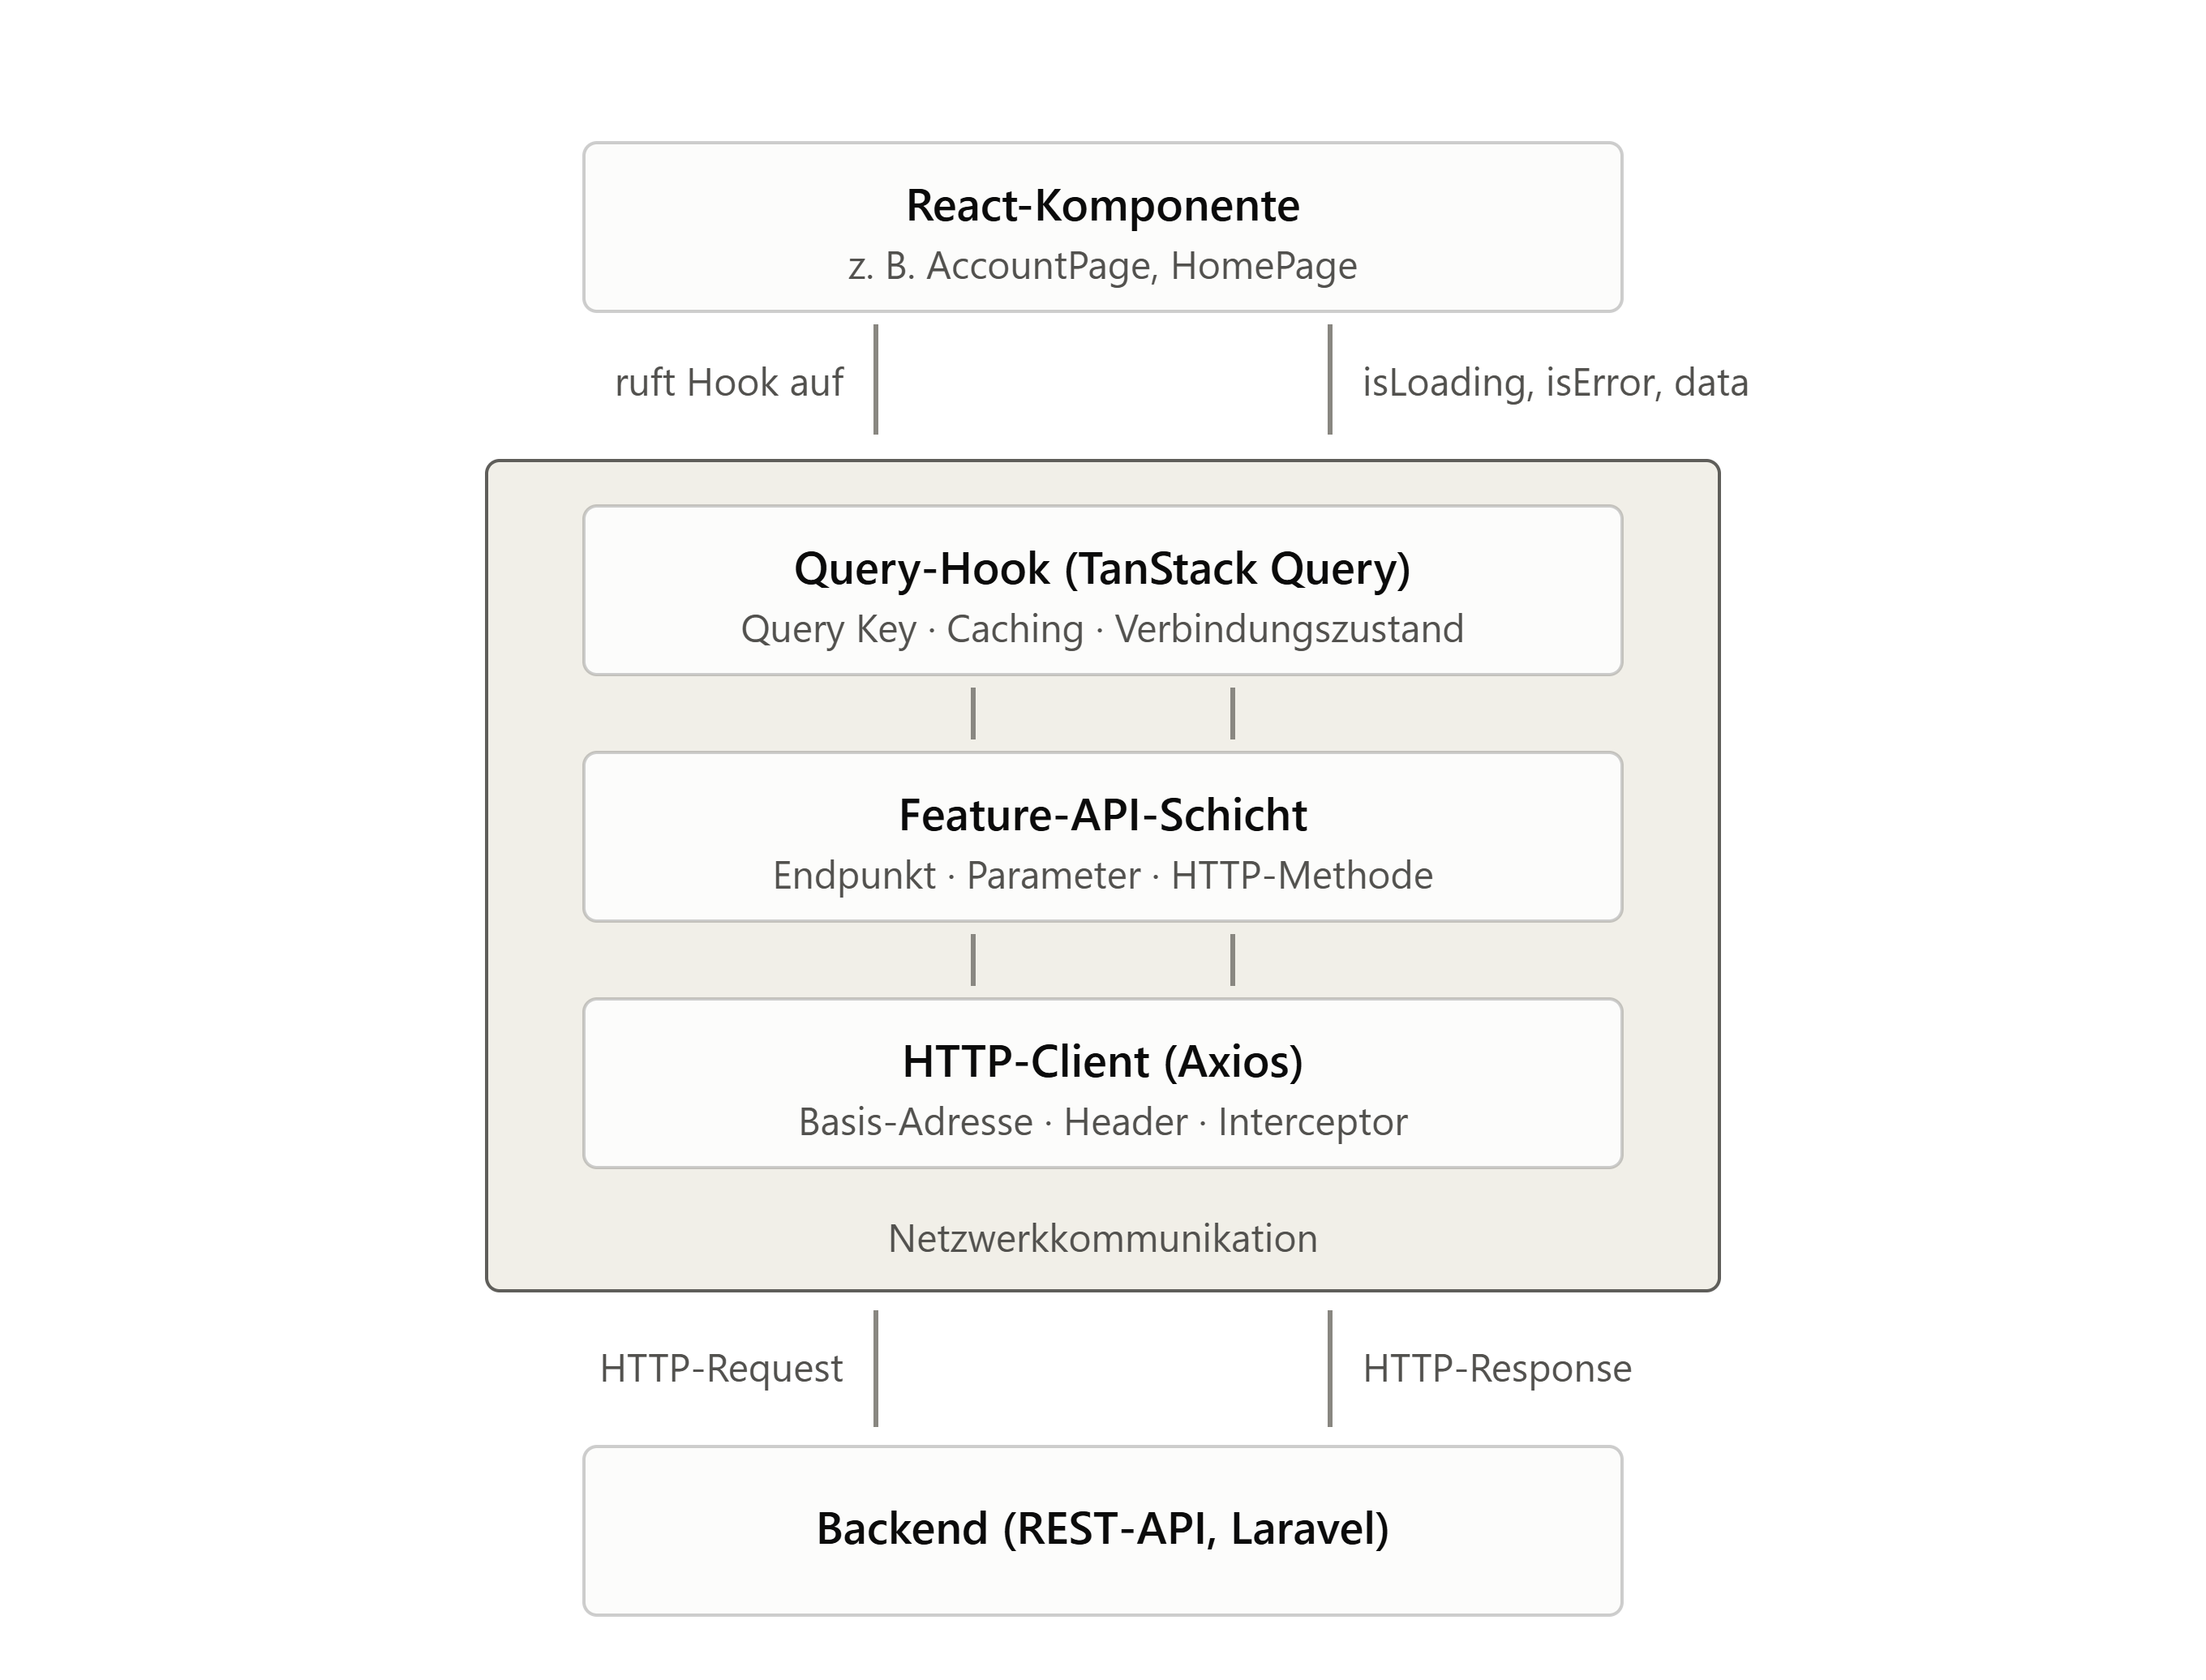
\includegraphics[width=0.75\textwidth]{Bilder/abb_netzwerk_schichten.png}
\caption{Drei-Schichten-Modell der Netzwerkkommunikation im Frontend von Bazario}
\label{fig:netzwerk_schichten}
\end{figure}



Ein wesentliches Ziel dieses Konzepts ist die einheitliche
Kontrolle über den Zustand jeder Verbindung. Jede Anfrage wird
dabei über einen Query Key identifiziert, der sich aus der
Bezeichnung der Anfrage und ihren Parametern zusammensetzt.
Trifft innerhalb eines kurzen Zeitraums dieselbe Anfrage mit
denselben Parametern erneut ein, erkennt TanStack Query, dass die
zugehörigen Daten bereits im Cache vorliegen, und liefert diese
zurück, anstatt den Server erneut zu kontaktieren; ändern sich
die Parameter, entsteht hingegen ein neuer Query Key und damit
eine neue Anfrage an den Server. Auf dieser Grundlage
unterscheidet die Bibliothek zwischen lesenden Anfragen, die
Daten vom Server abrufen, und schreibenden Operationen, die Daten
auf dem Server verändern. Darüber hinaus bietet
die Bibliothek einen Mechanismus zur gezielten Invalidierung
bereits abgerufener Daten; dieser bildet die projektweit
einheitliche Grundlage für die Aktualität zwischengespeicherter
Daten und wird in Kapitel~\ref{chap:umsetzung} anhand konkreter
Beispiele beschrieben.


Das beschriebene Konzept ergänzt das in
Abschnitt~\ref{subsec:state-management-konzept} dargestellte
globale State Management: Entsprechend der in
Abschnitt~\ref{subsec:state-management} eingeführten Trennung
verwaltet Zustand den clientseitigen Anwendungszustand, während
TanStack Query für den serverseitigen Datenbestand zuständig
ist, der über die beschriebenen Schichten abgerufen und
synchronisiert wird.


\section{UI/UX-Konzept}
\label{sec:uiux_konzept}
\subsection{Gestaltungsansatz und Leitlinien}
\label{subsec:gestaltungsansatz}
 
Die Oberfläche von \textit{Bazario} ist nicht als gestalterische
Schicht über der Anwendung entworfen, sondern als Teil ihrer
Struktur. Da die Plattform Produktkauf, Dienstleistungsbuchung,
Zahlung, Nachrichten und Kontoverwaltung in einem System vereint,
muss sie mehrere voneinander unabhängige Arbeitsabläufe tragen, ohne
dass die Bedienung mit jedem hinzukommenden Bereich unübersichtlicher
wird.
 
Maßgeblich für den Entwurf ist deshalb die Funktion einer Ansicht,
nicht ihr Erscheinungsbild. Jede Seite ist um diejenige Handlung
herum aufgebaut, die auf ihr im Vordergrund steht: Produktseiten um
das Sichten eines Angebots, Dienstleistungsseiten um die Wahl eines
Termins, Kontoseiten um die Verwaltung laufender Vorgänge. Das
Bedienmodell bleibt dadurch über die Anwendung hinweg gleich, auch
wenn die zugrunde liegenden Abläufe unterschiedlich komplex sind.
 
Die vier in Abschnitt~\ref{subsec:gestaltungsprinzipien} verdichteten
Anforderungen gelten dabei durchgehend: Konsistenz über gleichartige
Situationen hinweg, Erkennbarkeit des Systemzustands, Vermeidung von
Fehleingaben und Kontrolle des Nutzers über den Ablauf.
 
Hinzu tritt eine fünfte Leitlinie, die sich aus dem Rollenmodell
ergibt und in den allgemeinen Prinzipienkatalogen nicht vorkommt:
Rollensensitivität. Kunde, Verkäufer und Dienstleister rufen dieselbe
Anwendung aus unterschiedlichen Gründen auf. Einen Kunden beschäftigen
Katalog, Bestellung und Buchung; einen Verkäufer seine Produkte, die
eingegangenen Bestellungen und die Einnahmen; einen Dienstleister
zusätzlich Verfügbarkeit und Terminanfragen. Die Oberfläche gewichtet
daher je nach zugewiesener Rolle anders, ohne das gemeinsame
gestalterische System zu verlassen: Es ändert sich, was zuerst
erscheint, nicht wie es aussieht (vgl.
Abschnitt~\ref{subsec:verkaeufer_dashboard_konzept}).
 
Aus diesem Ansatz folgen vier Vorgaben, die den in den nächsten
Abschnitten beschriebenen Entscheidungen zugrunde liegen:
 
\begin{itemize}
\item Wiederkehrende Muster -- Karten, Schaltflächen, Dialoge,
      Zustandsmarkierungen, Formularabschnitte -- folgen denselben
      Regeln, statt je Ansicht neu festgelegt zu werden.
\item Der jeweils nächste sinnvolle Schritt einer Seite ist
      hervorgehoben; ergänzende Angaben treten zurück.
\item Farbe trägt Bedeutung und wird nicht zur Verzierung eingesetzt.
\item Eine nicht verfügbare Handlung wird benannt und begründet,
      statt stillschweigend zu entfallen.
\end{itemize}
 
Die letzte Vorgabe wiegt schwerer, als sie zunächst wirkt: Sie
betrifft die Fristen für Stornierung und Verlegung ebenso wie nicht
belegbare Tage in der Terminauswahl und ist an beiden Stellen
unabhängig voneinander angewandt worden (vgl.
Abschnitt~\ref{subsec:verkaeufer_dashboard_konzept} und
Abschnitt~\ref{subsec:buchung_konzept}).
 
Ergänzend gilt ein Grundsatz der Beschränkung: Bestandteile, die
lediglich vorhandene Wege wiederholen, entfallen. Eine Fußzeile
etwa nähme üblicherweise Angaben zum Betreiber, Verweise auf soziale
Netzwerke und Schnellzugriffe auf -- Inhalte, die entweder bereits in
der Kopfzeile erreichbar sind oder für den Funktionsumfang der
Plattform keine Rolle spielen. Verzichtet wird damit nicht auf
Gestaltung, sondern auf Doppelung.

\subsection{Designsystem und Farbschema}
\label{subsec:designsystem}
Das Designsystem von \textit{Bazario} setzt das in
Abschnitt~\ref{subsec:designsysteme} beschriebene Prinzip um, die
visuellen Grundelemente einer Anwendung nicht in den Komponenten zu
verstreuen, sondern als benannte Werte an einer Stelle zu pflegen.
Umgesetzt ist dies über \acs{CSS}-Variablen, die in der globalen
Stildatei definiert und über die Tailwind-Konfiguration als
Utility-Klassen verfügbar gemacht werden (vgl.
Abschnitt~\ref{subsec:ui-bibliotheken}).
 
Die Farbwerte sind nicht als Einzelfarben benannt, sondern nach ihrer
Funktion in der Oberfläche. Jede Fläche besitzt einen zugehörigen
Vordergrundwert, etwa \texttt{background} mit \texttt{foreground},
\texttt{card} mit \texttt{card-foreground} oder \texttt{primary} mit
\texttt{primary-foreground}. Diese paarweise Definition stellt sicher,
dass Text und Hintergrund nicht unabhängig voneinander geändert
werden können und ein Kontrastverhältnis damit nicht versehentlich
verloren geht. Ergänzt wird das Schema um Tokens für Rahmen,
Eingabefelder und Fokusringe sowie um einen eigenen Wert
\texttt{destructive} für zerstörende Aktionen und Fehlerzustände.
 
Als Farbraum wird durchgängig \acs{OKLCH} verwendet. Anders als bei
hexadezimalen Angaben entspricht die Helligkeitskomponente dort
näherungsweise der wahrgenommenen Helligkeit, wodurch sich
Farbabstufungen gleichmäßig ableiten lassen \cite{css_color_4}. Die
Palette ist bewusst neutral gehalten: Sämtliche Flächen- und
Textfarben besitzen keinen Buntanteil, allein \texttt{destructive}
ist als roter Farbwert angelegt. Farbe wird damit ausschließlich dort
eingesetzt, wo sie eine Bedeutung trägt, während die inhaltliche
Gliederung über Helligkeit, Abstände und Typografie erfolgt.
 
Diese Zurückhaltung erklärt eine Entscheidung, die auf den ersten
Blick überrascht: Karten tragen dieselbe Flächenfarbe wie die Seite,
auf der sie liegen. Ihre Abgrenzung entsteht allein über den Rahmen.
Eine zweite Flächenfarbe hätte die Palette erweitert und müsste mit
sämtlichen darauf erscheinenden Texten und Schaltflächen abgestimmt
werden; der Rahmen leistet dieselbe Trennung, ohne einen weiteren
Farbwert einzuführen. Er ist deshalb bewusst nahe am Hintergrund
gewählt -- deutlich genug, um zu trennen, zurückhaltend genug, um
nicht mit dem Inhalt zu konkurrieren.
 
Der Wert \texttt{primary} kennzeichnet die jeweils vorrangige
Handlung einer Ansicht, also diejenige, die weitere Vorgänge erst
ermöglicht: die Anmeldung, das Auslösen des Checkouts, die Übernahme
einer Buchung in den Warenkorb. Handlungen ohne diese Wirkung
erhalten die zurückhaltendere Darstellung über \texttt{secondary} --
die Abmeldung etwa ist keine vorrangige Handlung und wird deshalb
anders dargestellt als die Anmeldung an derselben Stelle.
\texttt{muted} kennzeichnet Elemente ohne gegenwärtige Wirkung, also
insbesondere deaktivierte Schaltflächen.
 
Ein zweites vollständiges Token-Set ist für die dunkle Darstellung
hinterlegt und wird über eine Variante am Wurzelelement aktiviert.
Da die Komponenten ausschließlich die funktionalen Token
referenzieren und keine festen Farbwerte enthalten, erfordert der
Wechsel keine Änderung an den Komponenten selbst.
 
Die Eckenradien folgen demselben Prinzip. Definiert ist ein einziger
Basiswert von 0,625\,rem; die Abstufungen von klein bis sehr groß
ergeben sich daraus über feste Zuschläge in Schritten von vier
Pixeln. Dass überhaupt mehrere Stufen nötig sind, liegt an der
Wahrnehmung: Derselbe Radius wirkt an einer bildschirmbreiten Fläche
kaum, an einer kleinen Schaltfläche dagegen stark. Elemente
vergleichbarer Größe erhalten deshalb denselben Wert, größere und
kleinere jeweils eine benachbarte Stufe.
 
Für die Typografie wird mit \textit{Geist} eine variable Schriftart
eingebunden und über die Tokens für Fließtext und Überschriften
referenziert. Die Größen folgen einer Staffel: Seitentitel benennen
die aufgerufene Ansicht, Abschnittstitel gliedern sie, Kartentitel
bezeichnen einzelne Gegenstände wie Bestellungen oder
Dienstleistungen; darunter stehen der Fließtext in einer einzigen
Größe sowie gedämpfte Angaben für Metadaten und Hilfetexte. Die
Unterscheidung erfolgt dabei nicht ausschließlich über die Größe:
Wo zwei Angaben gleich groß erscheinen, etwa eine Feldbeschriftung
und der zugehörige Hinweis, trennt sie die Farbe. Diese Staffelung ist
auf den Konto- und Bestellseiten maßgeblich, wo zahlreiche
gleichrangig wirkende Angaben nebeneinander stehen und ohne
Gliederung schwer zu überblicken wären.
 
Das Farbschema und die Komponentenbasis entsprechen der neutralen
Standardkonfiguration von shadcn/ui \cite{shadcn_docs}. Diese wurde
übernommen, weil sie die in Abschnitt~\ref{subsec:designsysteme}
genannten Anforderungen an Konsistenz bereits erfüllt; eine eigene
Gestaltung der Grundelemente war für den Funktionsumfang dieser
Arbeit nicht erforderlich.
 
Die paarweise Definition von Fläche und Vordergrund erlaubt es, die
Anforderungen aus Abschnitt~\ref{subsec:barrierefreiheit} unmittelbar
am Farbsystem zu prüfen. Für den Fließtext auf heller Fläche ergibt
sich ein Kontrastverhältnis von 19,8:1, für gedämpften Text 4,6:1;
beide erfüllen Erfolgskriterium 1.4.3 der Stufe AA. Für
Bedienelemente und Zustandsanzeigen gilt mit Kriterium 1.4.11 ein
eigener Schwellenwert von 3:1, dessen Prüfung in
Kapitel~\ref{chap:testen} erfolgt.


\subsection{Seitenstruktur und Navigationsprinzip}
\label{subsec:seitenstruktur}
Sämtliche Ansichten der Anwendung sind in einen gemeinsamen Rahmen
eingefasst, der aus der in Abschnitt~\ref{subsec:routing-konzept}
beschriebenen Routenhierarchie folgt: Die Layout-Komponente bildet
die oberste Ebene, alle Seiten werden als deren Kindrouten
dargestellt. Was sich beim Wechsel einer Seite ändert, ist damit
allein der Inhaltsbereich; die Kopfzeile bleibt bestehen.
Abbildung~\ref{fig:rahmen} zeigt diesen Aufbau.
 
\begin{figure}[H]
\centering
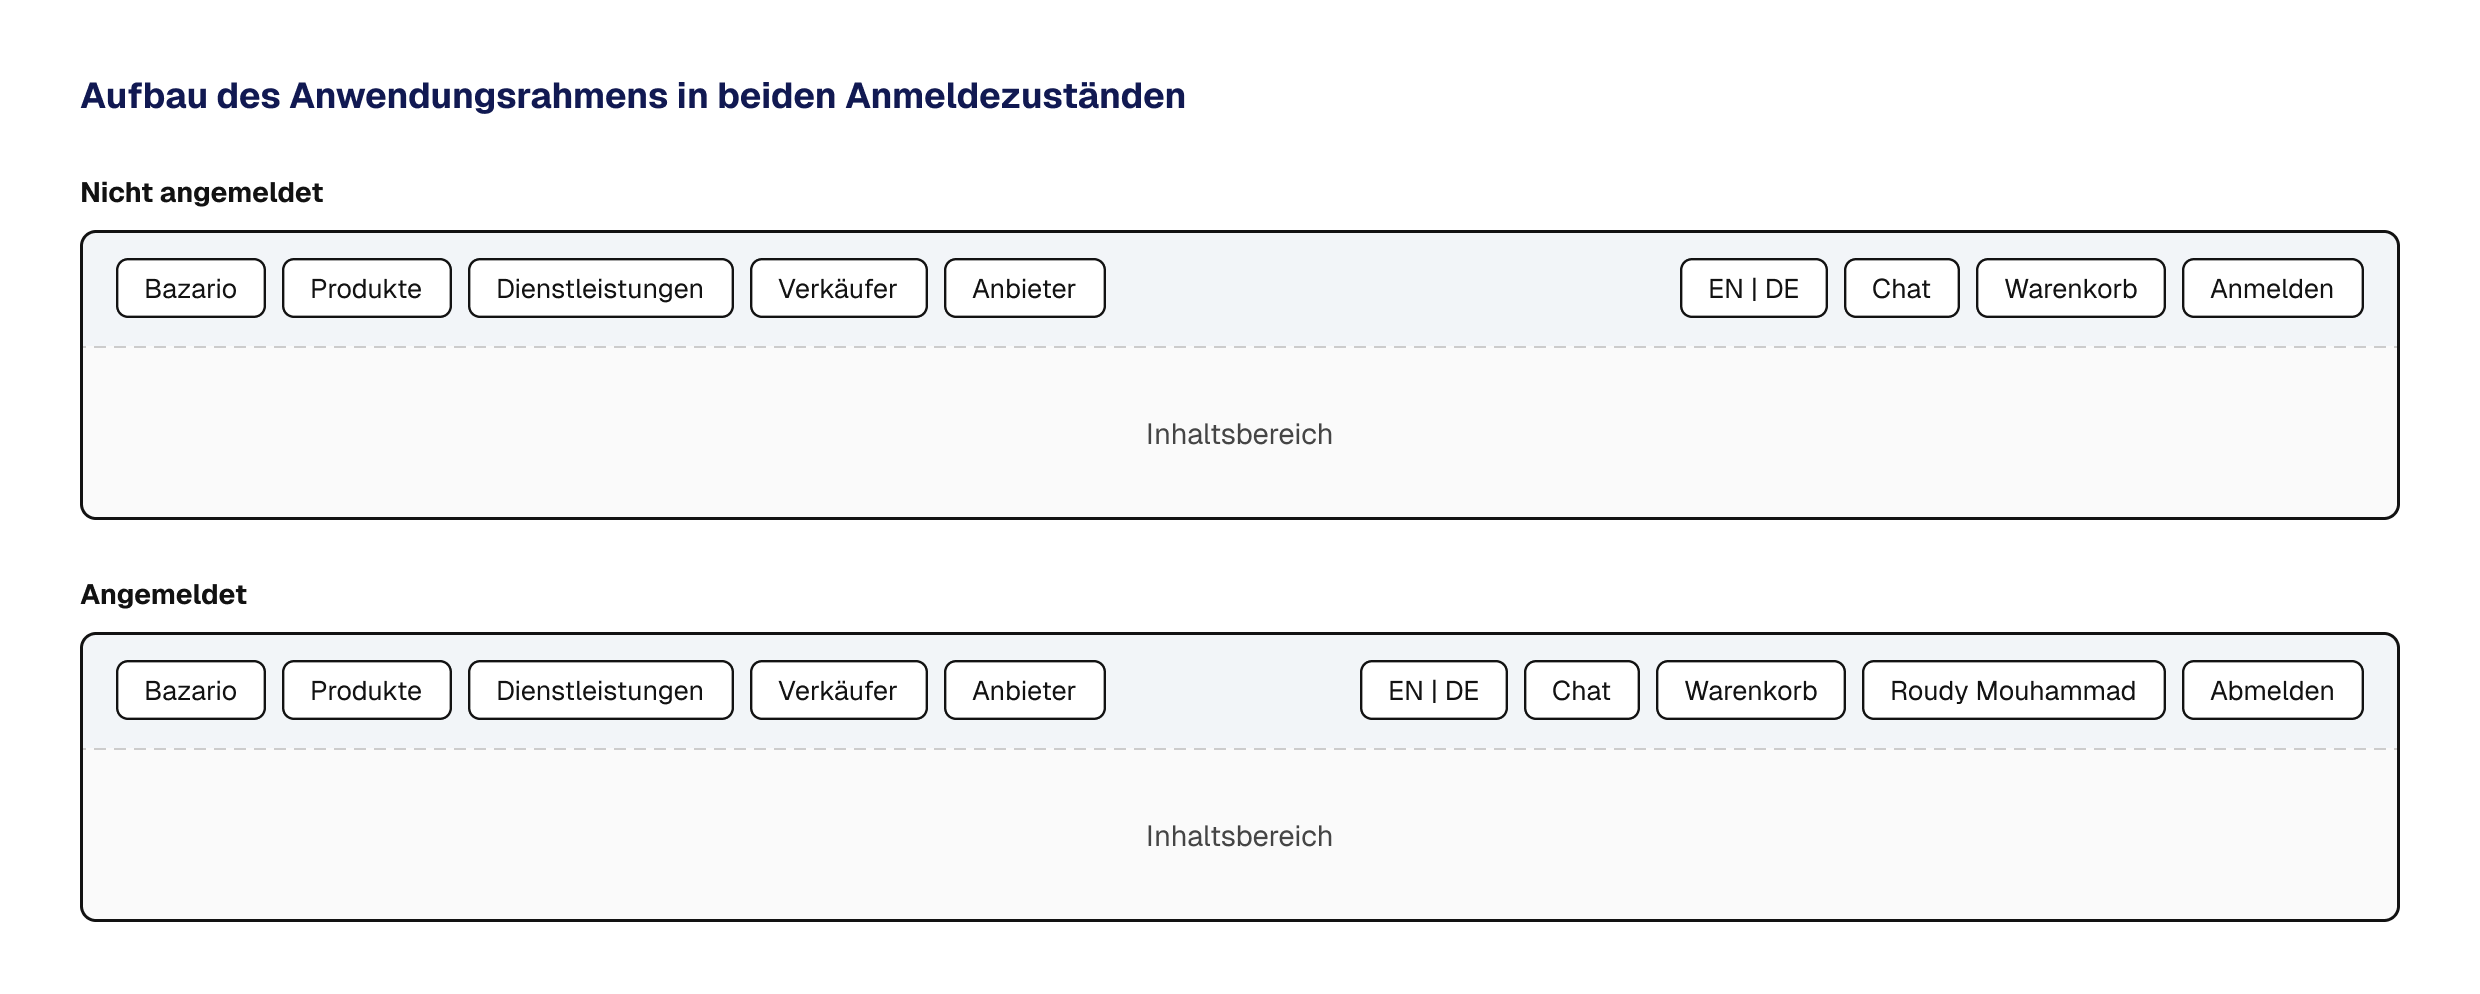
\includegraphics[width=0.80\textwidth]{Bilder/abb_rahmen.png}
\caption{Aufbau des Anwendungsrahmens in beiden Anmeldezuständen
(Strukturskizze, eigene Darstellung)}
\label{fig:rahmen}
\end{figure}
 
Die Kopfzeile ist in zwei Gruppen geteilt. Links steht neben dem
Namen der Plattform die fachliche Navigation mit den vier
öffentlichen Katalogbereichen -- Produkte, Dienstleistungen,
Verkäufer und Anbieter (vgl.
Abschnitt~\ref{subsec:katalog_konzept}). Rechts stehen die
Werkzeuge, die den Nutzer selbst betreffen: die Sprachwahl (vgl.
Abschnitt~\ref{subsec:mehrsprachigkeit_konzept}), der Zugang zu den
Nachrichten (vgl. Abschnitt~\ref{subsec:messaging_konzept}), der
Warenkorb und der Kontobereich.
 
Zwischen den beiden Anmeldezuständen ändert sich nur diese rechte
Gruppe: An die Stelle der Schaltfläche zur Anmeldung treten der Name
des Nutzers und die Abmeldung. Die fachliche Navigation bleibt
unverändert, da die Katalogbereiche allen Nutzern offenstehen. Der
Rahmen erfüllt damit die in
Abschnitt~\ref{subsec:gestaltungsprinzipien} genannte Anforderung
nach Konsistenz über gleichartige Situationen hinweg: Ein Nutzer, der
sich anmeldet, findet dieselbe Oberfläche vor und muss sich nicht neu
orientieren.
 
Eine Fußzeile besteht nicht (vgl.
Abschnitt~\ref{subsec:gestaltungsansatz}); der Inhaltsbereich endet
mit dem letzten Abschnitt der jeweiligen Seite, sodass sämtliche
Navigation an einer einzigen Stelle zusammenläuft.
 
Wie sich eine konkrete Seite in diesen Rahmen einfügt, zeigt
Abbildung~\ref{fig:startseite} am Beispiel der Startseite.
 
\begin{figure}[H]
\centering
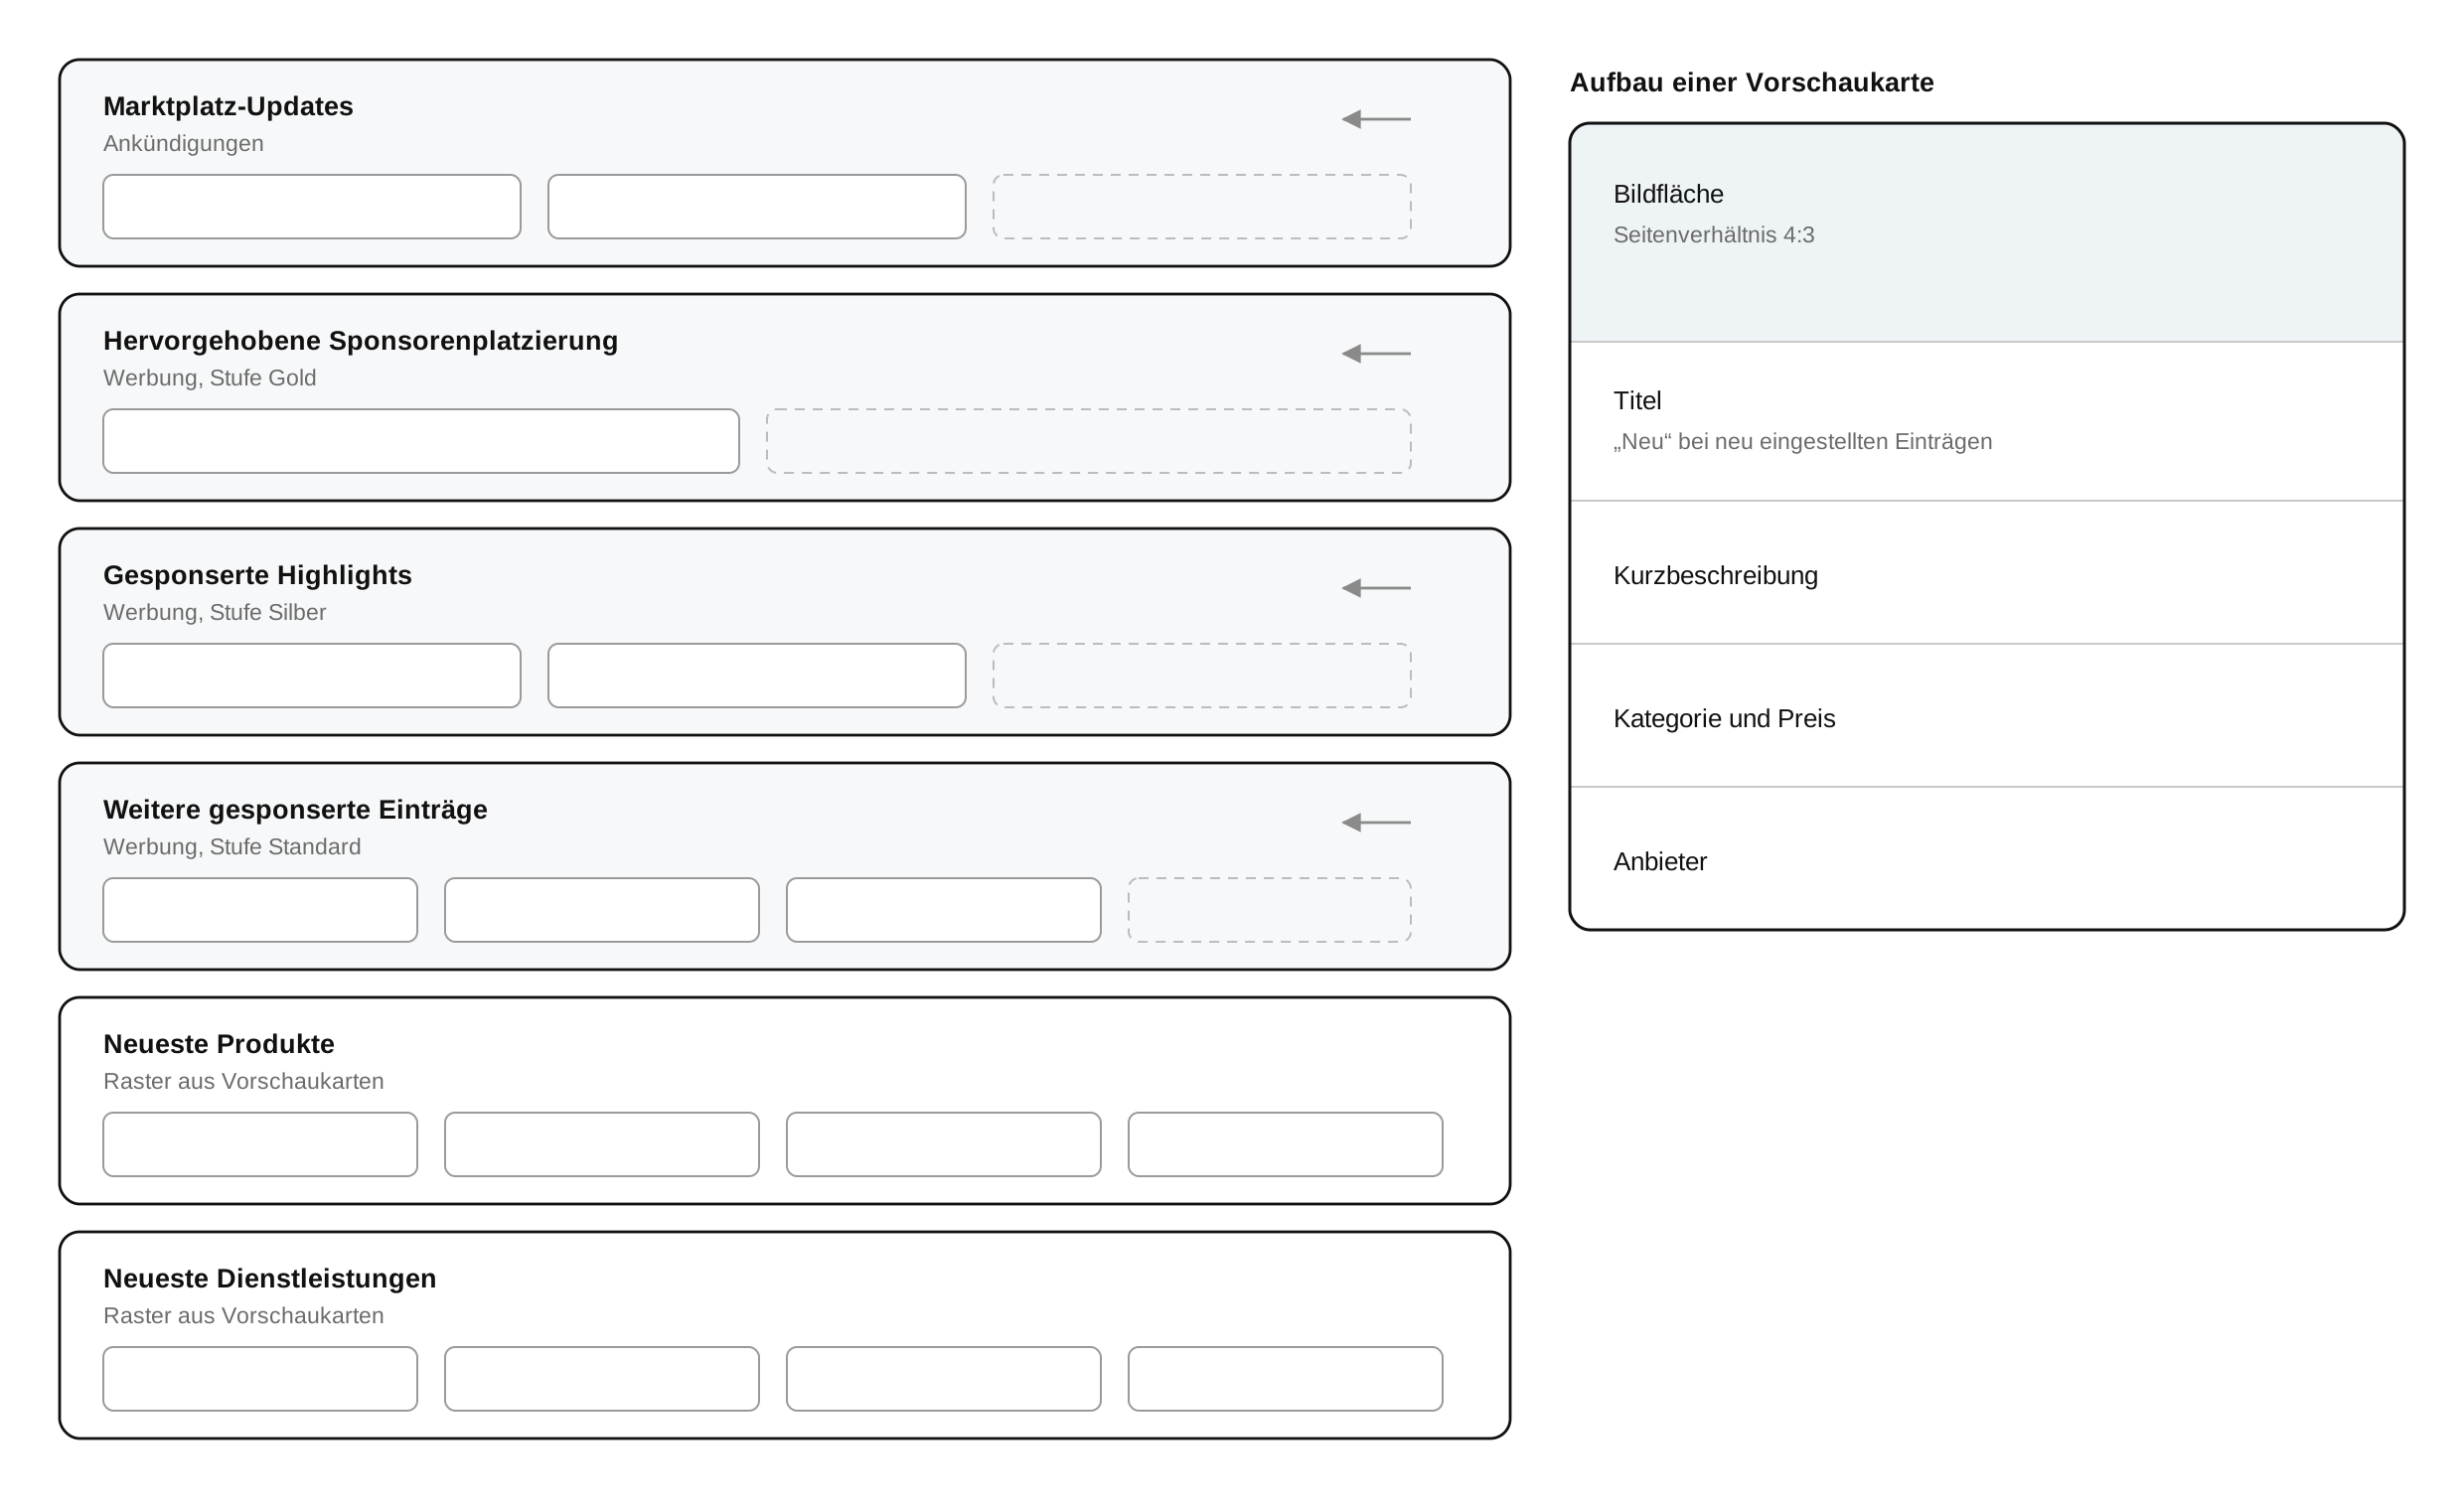
\includegraphics[width=\textwidth]{Bilder/abb_startseite.png}
\caption{Struktur der Startseite und Aufbau einer Vorschaukarte
(Strukturskizze, eigene Darstellung)}
\label{fig:startseite}
\end{figure}
 
Auf den Seitentitel mit einem einleitenden Satz folgen zwei
gleichartig aufgebaute Abschnitte, einer für die zuletzt
eingestellten Produkte und einer für die zuletzt eingestellten
Dienstleistungen. Beide bestehen aus einer Überschrift und einem
Raster aus Vorschaukarten.
 
Die Karte ist dabei das durchgehende Gestaltungselement des
Katalogbereichs. Sie führt von oben nach unten die Bildfläche, den
Titel, eine Kurzbeschreibung, die Kategorie zusammen mit dem Preis
und schließlich den Anbieter. Produkte und Dienstleistungen
verwenden dieselbe Karte in derselben Anordnung; sie unterscheiden
sich allein in der Hintergrundfarbe der Bildfläche. Dieselbe Karte
wird auf den Katalogseiten und den Profilseiten der Anbieter erneut
verwendet, sodass ein Angebot überall in derselben Form erscheint --
die technische Grundlage dafür bildet das in
Abschnitt~\ref{subsec:komponentenarchitektur} beschriebene
Komponentenmodell.
 
Die Zahl der Karten je Zeile richtet sich nach der verfügbaren
Anzeigefläche und verringert sich auf schmalen Bildschirmen, ohne
dass der Aufbau der einzelnen Karte sich ändert. Das entspricht dem
in Abschnitt~\ref{subsec:responsive-design} beschriebenen Vorgehen,
die Anordnung der Elemente an Umbruchpunkten anzupassen, statt eine
zweite Oberfläche vorzuhalten.
 
Auf schmalen Anzeigeflächen ändert sich jedoch nicht nur die
Spaltenzahl. Die Kopfzeile trägt nebeneinander die Navigation, die
Sprachwahl, den Zugang zu Nachrichten und Warenkorb sowie den
Kontobereich; auf geringer Breite würde diese Reihe umbrechen und die
Bedienung erschweren. Sie wird deshalb unterhalb eines Umbruchpunkts
zu einem aufklappbaren Menü zusammengefasst, sodass die obere Leiste
kompakt bleibt.
 
Ebenso ändert sich die Reihenfolge innerhalb der Karten. Eine
Anordnung, die auf breiter Fläche übersichtlich wirkt, führt auf
schmaler entweder zu übermäßiger Breite oder zu leeren Bereichen.
Titel, Preis, Zeitangabe und die zugehörige Handlung bleiben deshalb
zuerst sichtbar, während ergänzende Angaben darunter rücken. Die
Terminauswahl ist dabei der empfindlichste Fall: Tageswahl,
Zeitfensterliste, Zeitzone und Zusammenfassung müssen auch auf
geringer Breite zusammenhängend erkennbar bleiben, da eine
unvollständig erfasste Auswahl unmittelbar zu einer falschen Buchung
führen würde.
 
Am Fuß der Seite ist ein Bereich für Werbung und Ankündigungen
vorgesehen; er ist in Abbildung~\ref{fig:startseite} gestrichelt
dargestellt.

\subsection{Barrierefreiheit im Entwurf}
\label{subsec:barrierefreiheit_konzept}
 
Barrierefreiheit ist im Entwurf als Qualitätsanforderung behandelt,
nicht als Nachweisziel. Maßgeblich sind die vier in
Abschnitt~\ref{subsec:barrierefreiheit} genannten Erfolgskriterien;
ihre Prüfung erfolgt in Kapitel~\ref{chap:testen}.
 
Vier Festlegungen ergeben sich daraus für den Entwurf.
 
Erstens werden Bedienelemente ihrer Bedeutung entsprechend gewählt:
Navigation als Verweis, eine auslösende Handlung als Schaltfläche,
eine Rückfrage als Dialogkomponente und nicht als browsereigene
Abfrage. Damit ist die Bedeutung eines Elements nicht nur visuell,
sondern auch im Dokument hinterlegt und für assistive Technologien
zugänglich. Handlungen mit nicht umkehrbarer Wirkung -- das Löschen
einer Dienstleistung, eines Produkts oder des eigenen Kontos --
werden zusätzlich über einen Bestätigungsdialog geführt, sodass der
Nutzer die Kontrolle über den Ablauf behält (vgl.
Abschnitt~\ref{subsec:gestaltungsprinzipien}).
 
Zweitens erhält jedes bedienbare Element einen sichtbaren
Fokuszustand. In Abläufen mit mehreren aufeinanderfolgenden
Bedienschritten -- Anmeldung, Terminauswahl, Kontoverwaltung -- muss
ohne Zeigegerät erkennbar bleiben, welches Element gerade angesteuert
ist.
 
Drittens tragen Eingabefelder eine eigene Beschriftung statt
lediglich eines Platzhaltertextes, und Fehlermeldungen erscheinen an
einer festen Stelle unterhalb des betroffenen Feldes. Ein
Platzhalter verschwindet mit der ersten Eingabe; die Angabe, was das
Feld erwartet, wäre damit genau dann nicht mehr verfügbar, wenn sie
überprüft werden soll.
 
Viertens bleibt eine nicht verfügbare Handlung sichtbar und wird
begründet, statt entfernt zu werden. Diese bereits in
Abschnitt~\ref{subsec:gestaltungsansatz} genannte Vorgabe hat hier
eine zweite Begründung: Ein Bedienelement, das erst nach dem Auslösen
fehlschlägt, teilt den Systemzustand später mit als eines, das seinen
Zustand von vornherein anzeigt.
\subsection{Mehrsprachigkeit und Sprachwahl}
\label{subsec:mehrsprachigkeit_konzept}
 
\textit{Bazario} folgt der in
Abschnitt~\ref{subsec:mehrsprachigkeit} beschriebenen Zweiteilung:
Die Oberflächentexte werden im Frontend übersetzt, die Angaben zu
Produkten, Dienstleistungen und Anbietern liefert das Backend bereits
in der angeforderten Sprache. Diese Aufteilung folgt aus der Herkunft
der Daten, nicht aus einer Entwurfsentscheidung -- ein Anbieter
erfasst Titel und Beschreibung mehrsprachig (vgl.
Abschnitt~\ref{subsec:verkaeufer_dashboard_konzept}), weshalb nur das
Backend beide Fassungen kennt.
 
Die Sprachwahl ist im Anwendungsrahmen angeordnet und damit von jeder
Seite aus erreichbar. Sie wirkt ohne erneutes Laden, da ein Neuladen
den Zustand der Ansicht verwerfen würde, etwa eine begonnene Eingabe.
Beim ersten Aufruf gilt die im Browser eingestellte Sprache, sofern
sie unterstützt wird, andernfalls Englisch; die anschließend
getroffene Wahl wird gespeichert und bei späteren Besuchen
wiederhergestellt.
 
Angeboten werden Deutsch und Englisch, für die Oberflächentexte
vollständig umgesetzt. Bei den Inhalten reicht die Wahl gegenwärtig
nicht so weit: Die Erfassungsformulare sehen Englisch und Arabisch
vor, sodass eine deutsche Fassung nicht entsteht. Anforderung und
Verfügbarkeit einer Sprache sind damit zwei getrennte Fragen -- das
Frontend kann jede Sprache anfordern, geliefert wird nur, was zuvor
erfasst wurde.

% ----------------------------------------------------------------
\section{Konzept der einzelnen Funktionsbereiche}
\subsection{Authentifizierung und Onboarding}
\label{subsec:auth-onboarding}

Der Login erfolgt über einen Dialog, der von
jeder Stelle der Anwendung aus aufgerufen werden
kann, ohne die aktuelle Seite zu verlassen,
sodass ein Nutzer etwa während des Checkouts
nicht unterbrochen wird. Die Registrierung
erfolgt dagegen über eine eigene Seite, da sie
mehr Eingabefelder benötigt und eine
eigenständige Handlung darstellt. Beide
Formulare validieren ihre Eingaben clientseitig,
bevor eine Anfrage gestellt wird; serverseitige
Fehler werden gezielt dem betroffenen Feld
zugeordnet, und der Absende-Button wird während
der Bearbeitung deaktiviert.

Verläuft Anmeldung oder Registrierung
erfolgreich, bildet die Anwendung aus der
Backend-Antwort eine Sitzung mit
Zugriffstoken, Nutzerdaten und Rollen. Diese wird
im localStorage gespeichert, um den Anmeldestatus
über Neuladen und erneute Besuche hinweg zu
erhalten, und reaktiv über Zustand
bereitgestellt (vgl.
Abschnitt~\ref{subsec:state-management-konzept}).
Der Zugriff auf geschützte Bereiche wird über ein
dreistufiges Konzept sichergestellt: Zunächst
wird geprüft, ob der Anmeldestatus bereits
bestimmt ist (Ladezustand), dann ob der Nutzer
angemeldet ist (sonst Weiterleitung), und erst
danach wird der geschützte Inhalt angezeigt.

Der gespeicherte Token wird automatisch über
einen zentralen, wiederverwendbaren Mechanismus
an jede Anfrage angehängt und zusätzlich aktiv
beim Backend validiert, sodass ein abgelaufener
oder ungültiger Token erkannt und der Nutzer
korrekt abgemeldet wird. Für das Onboarding
verfolgt die Plattform ein zweistufiges
Rollenmodell: Jeder Nutzer erhält zunächst die
Rolle \textit{Customer}, ein Wechsel zu \textit{Seller} oder
\textit{ServiceProvider} erfolgt über einen von einem
Administrator geprüften Antragsprozess.
 
 
 
\subsection{Katalog- und Detailseiten}
\label{subsec:katalog_konzept}

Der Katalogbereich von \textit{Bazario}
umfasst die Startseite, die
Katalogseiten für Produkte und
Dienstleistungen sowie die öffentlichen
Profilseiten einzelner Verkäufer und
Dienstleister.

Die Startseite fasst Ankündigungen, Werbeplatzierungen sowie
eine Vorschau der zuletzt hinzugefügten Produkte und
Dienstleistungen in aufeinanderfolgenden Abschnitten zusammen.
Sämtliche Inhalte der Startseite werden über eine einzelne,
gebündelte Anfrage an das Backend abgerufen.

Über eigenständige Katalogseiten
lassen sich alle Produkte
beziehungsweise Dienstleistungen der
Plattform einsehen und nach Kategorie
filtern. Zusätzlich
stellt \textit{Bazario} für jeden
Verkäufer und jeden Dienstleister eine
öffentliche Profilseite bereit, auf
der Kunden ausschließlich die Produkte
beziehungsweise Dienstleistungen
dieses einen Anbieters einsehen
können. Diese öffentlichen
Profilseiten sind von der internen
Verwaltungsseite des jeweiligen
Verkäufers oder Dienstleisters zu
unterscheiden, die in
Abschnitt~\ref{subsec:verkaeufer_dashboard_konzept}
beschrieben wird.

Der Aufruf eines einzelnen Produkts
oder einer einzelnen Dienstleistung,
etwa über eine Vorschau-Karte, führt
jeweils auf eine eigene Detailseite.
Für die Darstellung der Vorschauen auf
Startseite und Katalogseiten wird ein
wiederverwendbares Kartenprinzip
verfolgt, das für Produkte und
Dienstleistungen gleichermaßen zum
Einsatz kommt; liegen für einen
Bereich keine Einträge vor, wird dem
Nutzer anstelle einer leeren Fläche
ein entsprechender Hinweis angezeigt.


\subsection{Dienstleistungsbuchung}
\label{subsec:buchung_konzept}
Eine Dienstleistung wird nicht wie ein Produkt in den Warenkorb
gelegt, sondern zuvor auf einen konkreten Termin festgelegt. Der
Entwurf muss daher eine Auswahl anbieten, die nur solche Zeitpunkte
enthält, an denen die Leistung tatsächlich erbracht werden kann.
 
Welche Zeitpunkte das sind, ergibt sich aus zwei Gruppen von Angaben,
die beide in Abschnitt~\ref{subsec:verkaeufer_dashboard_konzept}
beschrieben sind. Die erste betrifft den Anbieter als Person: sein
wiederkehrendes Wochenschema und seine eingetragenen
Abwesenheitszeiträume. Die zweite betrifft die einzelne
Dienstleistung: ihre Dauer, das Zeitraster, in dem Termine beginnen
dürfen, und die Anzahl der Kunden, die denselben Zeitraum belegen
können. Hinzu kommen die bereits vergebenen Buchungen. Die Menge der
wählbaren Termine ist damit nicht fest hinterlegt, sondern wird für
jeden Tag neu bestimmt.
 
Die Auswahl erfolgt in zwei Schritten: zuerst der Tag, dann das
Zeitfenster. Eine gemeinsame Liste aller Termine über mehrere Wochen
hinweg wäre unübersichtlich, und die Zahl der Einträge stiege mit
einem feineren Zeitraster weiter an. Erst nach der Wahl eines Tages
werden dessen Zeitfenster abgerufen und angezeigt.
 
Zu jedem Zeitfenster wird die verbleibende Kapazität angegeben. Bei
Dienstleistungen, die mehrere Kunden gleichzeitig annehmen können,
ist andernfalls nicht erkennbar, ob eine Buchung noch möglich ist
oder das Fenster lediglich noch nicht ausgebucht wirkt.
 
Sämtliche Zeitangaben beziehen sich auf die Zeitzone des Anbieters,
die zusammen mit dem Termin angezeigt wird. Da Anbieter und Kunde in
verschiedenen Zeitzonen ansässig sein können, wäre eine Angabe ohne
Bezugspunkt mehrdeutig; die Zeitzone des aufrufenden Endgeräts als
Grundlage zu verwenden, würde die Angaben je nach Standort des Kunden
verschieben.
 
Die abgeschlossene Auswahl führt nicht unmittelbar zu einer Buchung,
sondern in den Warenkorb. Damit lassen sich Dienstleistungen und
Produkte in einem gemeinsamen Vorgang bezahlen (vgl.
Abschnitt~\ref{subsec:warenkorb_konzept}), und eine verbindliche
Buchung entsteht erst mit der Zahlung. Solange der Vorgang nicht
abgeschlossen ist, bleibt das Zeitfenster für andere Kunden verfügbar.

\subsection{Warenkorb, Checkout und Zahlung}
\label{subsec:warenkorb_konzept}

Der Warenkorb bildet Produkte und Dienstleistungsbuchungen in
einem gemeinsamen Modell ab, das für beide Positionstypen eine
gemeinsame Basis aus Titel, Bild, Preis und Kategorie sowie
typspezifische Zusatzdaten vorsieht; eine Dienstleistungsbuchung
enthält zusätzlich Beginn, Ende, Zeitzone und Ort der
Leistungserbringung. Der Warenkorb bleibt über einen erneuten
Aufruf der Anwendung hinweg erhalten, sodass bereits
hinzugefügte Positionen auch nach einem Neuladen der Seite
bestehen bleiben. Wird ein bereits enthaltenes Produkt erneut
hinzugefügt, erhöht sich lediglich dessen Menge; eine identische
Dienstleistungsbuchung kann dagegen nicht doppelt hinzugefügt
werden. Die Warenkorbseite gliedert sich in eine Übersicht der
enthaltenen Positionen, getrennt nach Produkten und
Dienstleistungen, sowie eine Zusammenfassung mit Anzahl je
Positionstyp und Zwischensumme.

Der Checkout setzt eine angemeldete Sitzung voraus. Ist der Nutzer
nicht angemeldet, öffnet sich der in
Abschnitt~\ref{subsec:auth-onboarding} beschriebene Anmeldedialog,
bevor der Vorgang fortgesetzt wird. Die Plattform muss den Vorgang
einem Nutzer zuordnen können, um ihn nachverfolgbar zu machen, dem
Anbieter mitzuteilen, wer bestellt hat, und dem Kunden die Einsicht in
seine Bestellungen zu ermöglichen.
 
Ein Auftrag entsteht bereits vor der Zahlung. Mit dem Auslösen des
Checkouts legt das Backend einen Auftrag mit dem Status
\textit{requires payment} an, ergänzt ihn um die Positionen des
Warenkorbs und fordert anschließend eine Zahlungssitzung an. Bricht
der Nutzer die Zahlung ab, bleibt der Auftrag unbezahlt bestehen und
kann später über die Bestellübersicht abgeschlossen werden. Der
Warenkorb bleibt in diesem Fall unverändert erhalten, damit ein
abgebrochener Vorgang nicht zum Verlust der bereits
zusammengestellten Positionen führt.
 
Von den in Abschnitt~\ref{subsec:online-zahlung} beschriebenen
Einbindungsvarianten nutzt \textit{Bazario} die gehostete
Zahlungsseite (vgl. Abschnitt~\ref{sec:technologieauswahl}). Das
Frontend gestaltet damit keine eigenen Zahlungsformulare, und
sensible Kartendaten erreichen die Plattform zu keinem Zeitpunkt.

Darin liegt zugleich die Begründung für die
eingangs genannte Anmeldepflicht: Plattformen, die einen Kauf ohne
Anmeldung zulassen, wickeln die Zahlung selbst ab und erhalten dabei
zwangsläufig die Daten des Kunden. Bei \textit{Bazario} gehen diese
Daten ausschließlich an den Zahlungsdienst; ohne Anmeldung läge der
Plattform daher keinerlei Information über den Vorgang vor.
 
Dieser Weg hat eine Konsequenz für den Entwurf: Sobald der Nutzer zur Zahlung auf die Seite des Zahlungsdienstes wechselt, verliert die Plattform die unmittelbare Sicht auf den Vorgang. Sie erfährt weder, ob gezahlt wurde, noch von wem. Genau deshalb wird der Auftrag vorab im Backend angelegt und der Zahlungsstatus im Anschluss beim Zahlungsdienst abgefragt \cite{stripe_checkout_docs}.
 
Die Kommunikation mit dem Zahlungsdienst erfolgt ausschließlich über
das Backend, nicht aus dem Browser heraus. Der Grund liegt in der
Authentifizierung gegenüber dem Dienst: Das Eröffnen einer
Zahlungssitzung erfordert einen geheimen Schlüssel, der dem
Plattformbetreiber zugeordnet ist und nicht im Browser des Nutzers
liegen darf. Hinzu kommt, dass die Plattform eine Vielzahl von Nutzern
bedient und die Eröffnung von Zahlungssitzungen kontrolliert erfolgen
muss.
 
Für die Rückleitung nach abgeschlossener oder abgebrochener Zahlung
stellt das Frontend zwei eigene Seiten bereit. Ihre Adressen werden dem
Zahlungsdienst über das Backend mitgeteilt, sodass der Nutzer nach dem
Verlassen der Zahlungsseite auf die passende Seite der Anwendung
zurückgeführt wird. Beide Seiten sind an eine gültige Sitzung
gebunden, da der Ausgang einer Zahlung einem bestimmten Nutzer
zugeordnet ist.
 
Damit Anbieter Zahlungen empfangen können, nutzt \textit{Bazario} das
Konzept verbundener Konten. Die Plattform unterhält ein eigenes Konto
beim Zahlungsdienst; jedem Verkäufer und jedem Dienstleister wird
darunter ein Unterkonto zugeordnet. Dieses Unterkonto wird aus der
Anwendung heraus angelegt, sodass der Anbieter kein eigenes Konto
einrichten und verknüpfen muss. Auf dieser Grundlage lässt sich der
Zahlungsbetrag automatisiert aufteilen: Ein Anteil verbleibt als
Provision bei der Plattform, der übrige Betrag wird dem Anbieter
gutgeschrieben (vgl. Abschnitt~\ref{subsec:marktplatztypen}).
 
Voraussetzung für eine Gutschrift ist ein vollständig eingerichtetes
Unterkonto einschließlich Identitätsprüfung. Solange diese Prüfung
nicht abgeschlossen ist, weist die Anwendung den Anbieter darauf hin
und zeigt weder Guthaben noch Transaktionen an. Die Einnahmenübersicht
stellt anschließend den Verbindungsstatus, das verfügbare Guthaben und
die noch ausstehenden Beträge dar. Die Auszahlung selbst wird über das
Administrationsdashboard des Backends ausgelöst und ist damit nicht
Gegenstand dieser Arbeit (vgl. Abschnitt~\ref{sec:abgrenzung}).


\subsection{Kontobereich und rollenspezifische Funktionen}
\label{subsec:verkaeufer_dashboard_konzept}

Die Kontoseite bildet den zentralen Einstiegspunkt für alle
angemeldeten Nutzer. Sie ergänzt die in
Abschnitt~\ref{subsec:auth-onboarding} beschriebenen Angaben zur
Sitzung um den Überblick über laufende Vorgänge und den Zugang zu den
rollenspezifischen Funktionen. Dafür gliedert sie sich in zwei
Spalten: links der Stand der eigenen Vorgänge, rechts die verfügbaren
Werkzeuge.
 
Die rechte Spalte ist dabei nach Rollen gegliedert, nicht nach
Funktionen. Jede zugewiesene Rolle erhält einen eigenen
Arbeitsbereich. Die Reihenfolge folgt der Häufigkeit des Zugriffs:
Die rollenspezifischen Arbeitsbereiche stehen oben, da sie der Grund
sind, aus dem ein Anbieter die Seite aufruft; der Kundenbereich, den
jeder Nutzer nach dem Rollenmodell aus
Abschnitt~\ref{sec:rollenmodell} ebenfalls besitzt, folgt darunter.
Im Folgenden wird er dennoch zuerst beschrieben, da er die
gemeinsame Grundlage aller Rollen bildet.
 
Zu jedem Eintrag der linken Spalte wird der aktuelle Zustand
angezeigt, bei Buchungen der Bearbeitungsstand, bei Bestellungen der
Zahlungsstatus und beim Zahlungsdienst der Verbindungszustand, und
daneben genau die Aktion, die in diesem Zustand möglich ist, etwa das
Bestätigen einer angefragten Buchung oder das Nachholen einer offenen
Zahlung. Der Systemzustand ist damit erkennbar, ohne dass eine
Detailansicht geöffnet werden muss (vgl.
Abschnitt~\ref{subsec:gestaltungsprinzipien}).
 
 
% --------------------------- KUNDE -------------------------------
 
Der Kundenbereich führt zur eigenen Bestellhistorie und zur
Verfolgung eigener Buchungen. Beide Ansichten werden getrennt
geführt, weil sich Bestellungen und Buchungen in ihrem Zustandsumfang
deutlich unterscheiden: Ein Produkt wird bestellt, bezahlt und
geliefert, während eine Buchung zusätzlich einen Termin, eine
Zeitzone und die Möglichkeit zur Stornierung oder Verlegung besitzt.
 
Die Bestellübersicht führt sämtliche Aufträge des Nutzers mit
Zahlungsstatus, Datum, Gesamtbetrag und Anzahl der Positionen auf. Da
ein Auftrag bereits vor der Zahlung entsteht (vgl.
Abschnitt~\ref{subsec:warenkorb_konzept}), erscheinen dort auch
unbezahlte Aufträge. Für diese bietet die Übersicht zwei Wege an: die
Zahlung nachzuholen oder den Auftrag zu verwerfen. Ohne diese beiden
Möglichkeiten bliebe ein abgebrochener Zahlungsvorgang als Eintrag
bestehen, den der Nutzer weder abschließen noch entfernen könnte. Die
Detailansicht eines Auftrags zeigt darüber hinaus die einzelnen
Positionen und ihren jeweiligen Zustand.
 
Die Buchungsübersicht führt die gebuchten Termine mit
Bearbeitungsstand, Zeitpunkt und Ort. Zu jeder Buchung werden die
beim Anlegen der Dienstleistung festgelegten Fristen als
Buchungsbedingungen angezeigt, getrennt nach Stornierung und
Verlegung. Der Nutzer erfährt damit bereits vor einer Handlung, bis
wann sie möglich ist, und nicht erst beim Versuch. Nach Ablauf einer
Frist wird die zugehörige Schaltfläche deaktiviert und um eine
Erläuterung ergänzt, die den Grund und das Datum des Fristablaufs
benennt. Die Alternative, sie auszublenden, wurde verworfen: Ein
Nutzer, der eine erwartete Funktion nicht vorfindet, sucht sie
zunächst und erfährt nicht, warum sie fehlt. Die Frist markiert dabei nicht nur das Ende einer Bedienmöglichkeit, sondern den Übergang des wirtschaftlichen Risikos: Nach ihrem Ablauf steht der Betrag dem Anbieter zu, unabhängig davon, ob der Kunde die Leistung in Anspruch nimmt. Der Anbieter kennzeichnet die Buchung in
beiden Fällen nach dem Termin als abgeschlossen.
 
Eine Stornierung löst über das Backend eine Rückerstattung aus, deren
Stand in der Buchung nachvollziehbar bleibt. Eine Verlegung verändert
dagegen ausschließlich den Termin; der bezahlte Betrag bleibt
unberührt, weshalb hierfür ein eigener Auswahlschritt vorgesehen ist,
der die verfügbaren Zeitfenster des Anbieters anzeigt. Diese
Möglichkeiten bestehen ausschließlich für Dienstleistungen. Eine
bezahlte Produktbestellung lässt sich nicht mehr rückgängig machen,
da ihr keine terminierte Leistung zugrunde liegt, deren Absage einen
Zeitraum wieder freigäbe.
 
 
% ------------------------ DIENSTLEISTER --------------------------
 
Besitzt ein Nutzer zusätzlich die Rolle des Dienstleisters, tritt ein
Anbieterbereich hinzu. Er führt zur Verwaltung von Dienstleistungen
und Verfügbarkeiten, zu den eingegangenen Buchungen sowie zur
Anbindung an den Zahlungsdienst und zur Einnahmenübersicht (vgl.
Abschnitt~\ref{subsec:warenkorb_konzept}).
 
Die linke Spalte trennt entsprechend die Vorgänge, die andere Nutzer
beim Anbieter ausgelöst haben, von dessen eigenen Bestellungen;
andernfalls würden in einer Liste Vorgänge nebeneinander angezeigt
werden, bei denen der Nutzer einmal Anbieter und einmal Kunde ist.
Beide Listen zeigen nur die neuesten Einträge und verweisen für den
vollständigen Bestand auf eine eigene Seite.
Die eingegangenen Buchungen werden in einer eigenen Ansicht geführt,
da sie im Gegensatz zu Produktbestellungen eine Handlung des
Anbieters erfordern. Eine Buchung durchläuft dabei mehrere Zustände:
Sie erreicht den Anbieter zunächst als Anfrage, wird von ihm
bestätigt und nach erbrachter Leistung als abgeschlossen
gekennzeichnet.
 
Dass eine Buchung trotz bereits erfolgter Zahlung zunächst nur
angefragt ist, ist beabsichtigt. Die Zahlung sichert den Vorgang
finanziell ab, die Zusage über die Leistung selbst gibt jedoch der
Anbieter. Erst mit seiner Bestätigung gilt der Termin als
verbindlich.
 
Zu jeder Buchung werden daher Kunde, Zeitraum und Zeitzone angezeigt
sowie genau die Aktion, die im jeweiligen Zustand möglich ist: Eine
angefragte Buchung lässt sich bestätigen, eine bestätigte nach
erbrachter Leistung abschließen. Der Anbieter muss den Zustand einer
Buchung damit nicht aus dem Zusammenhang erschließen, sondern findet
an jedem Eintrag den nächsten möglichen Schritt (vgl.
Abschnitt~\ref{subsec:gestaltungsprinzipien}).
Der Abschluss ist dabei bewusst nicht an das Ende des Termins gebunden. In der Regel erfolgt er danach, doch teilt ein Kunde vorher mit, dass er die Leistung nicht in Anspruch nehmen wird, kann der Anbieter die Buchung bereits zuvor abschließen. Eine zeitliche Sperre hätte diesen Fall ausgeschlossen, ohne einen Fehler zu verhindern.
 
Dienstleister verwalten ihre Verfügbarkeit über feste
Arbeitszeiten sowie einzelne Abwesenheitszeiträume. Für jeden
Abwesenheitszeitraum werden Beginn und Ende sowie optional ein
Grund erfasst; zusätzlich lässt sich kennzeichnen, ob es sich um
einen offiziellen Feiertag oder eine persönliche Abwesenheit
handelt, damit Kunden bei der Buchung den Unterschied
nachvollziehen können. Da Dienstleister in unterschiedlichen
Zeitzonen tätig sein können, wird die Zeitzone des jeweiligen
Anbieters bei der Darstellung der Abwesenheitszeiten
berücksichtigt, sodass Zeitangaben nicht in der Zeitzone des
Endgeräts, sondern in der des Anbieters angezeigt werden.
Zusätzlich zu den einzelnen Abwesenheitszeiträumen legen
Dienstleister ein wiederkehrendes Wochenschema mit mehreren
Zeitfenstern je Wochentag fest, das die grundsätzliche
Erreichbarkeit unabhängig von einzelnen Abwesenheiten definiert.
 
Ihre einzelnen Dienstleistungsangebote verwalten Dienstleister
über eine Kartenübersicht, die für jede Dienstleistung Kategorie,
Preis, Dauer und Status anzeigt und das Anlegen, Bearbeiten und
Löschen einzelner Einträge ermöglicht. Titel und Beschreibung
einer Dienstleistung werden dabei jeweils auf Englisch und
Arabisch erfasst, und es lassen sich bis zu fünf Bilder je
Dienstleistung hochladen. Neben diesen Basisdaten legt ein
Dienstleister beim Anlegen oder Bearbeiten einer Dienstleistung
zusätzlich die Regeln für deren spätere Buchung fest: das
Zeitraster, in dem einzelne Termine gebucht werden können, die
maximale Anzahl gleichzeitiger Buchungen, den Ort der
Leistungserbringung sowie getrennte Fristen und Regelungen für
die Stornierung und die Änderung einer bereits bestätigten
Buchung durch den Kunden.
 
 
% -------------------------- VERKÄUFER ----------------------------
 
Für die Rolle des Verkäufers gilt dasselbe Prinzip. Auch hier tritt
ein eigener Arbeitsbereich hinzu, der zur Produktverwaltung sowie zu
Zahlungsdienst und Einnahmenübersicht führt, und auch hier erscheinen
die eingegangenen Bestellungen getrennt von den eigenen.
 
Verkäufer verwalten ihre Produkte über eine analoge
Kartenübersicht, die für jedes Produkt Kategorie und Preis
anzeigt und ebenfalls das Anlegen, Bearbeiten und Löschen
einzelner Einträge ermöglicht. Titel und Beschreibung werden
auch hier auf Englisch und Arabisch erfasst, mit bis zu fünf
Bildern je Produkt. Im Unterschied zu Dienstleistungen entfallen
dabei jedoch die Buchungsregeln.
 
 
% ------------------------ BEIDE ROLLEN ---------------------------
 
Besitzt ein Nutzer beide anbietenden Rollen, erscheinen deren
Arbeitsbereiche untereinander, jeweils zusätzlich zum Kundenbereich.
Nicht zugewiesene Rollen erzeugen dagegen keinen Arbeitsbereich,
sodass die Oberfläche ausschließlich die tatsächlich verfügbaren
Funktionen zeigt. Damit wird die in Abschnitt~\ref{subsec:rbac}
beschriebene rollenbasierte Zugriffskontrolle auf der Ebene der
Benutzerführung umgesetzt.
 
Unterhalb der Arbeitsbereiche folgen die rollenunabhängigen
Funktionen: Passwortänderung, Rollenwechselantrag und Kontolöschung.
Die Kontolöschung ist als eigener, farblich abgesetzter Bereich
angeordnet und benennt ihre Folgen vorab: Das Konto wird dauerhaft
deaktiviert, während abgeschlossene Bestellungen und die zugehörigen
Nachweise erhalten bleiben.

\subsection{Werbung und Ankündigungen}
\label{subsec:werbung_konzept}
% TODO: Ankündigungen je Rolle, produktspezifische Werbung,
% Genehmigungsprozesse.

\subsection{Messaging}
\label{subsec:messaging_konzept}
Der Nachrichtenbereich dient der Kommunikation in Echtzeit zwischen
einem Kunden und einem Verkäufer oder Dienstleister, etwa wenn der
Kunde vor einer Bestellung oder Buchung Fragen zu einem Produkt oder
einer Dienstleistung hat.
 
Die maßgebliche Anforderung ist dabei nicht der Austausch selbst,
sondern der Zeitpunkt: Eine Nachricht soll beim Empfänger erscheinen,
während er die Seite geöffnet hat, ohne dass er sie neu lädt. Damit
verlässt dieser Funktionsbereich als einziger das anfragebasierte
Modell, das allen übrigen Bereichen zugrunde liegt. Wie in
Abschnitt~\ref{subsec:rest-api} dargestellt, geht bei \acs{REST}
jede Übertragung vom Client aus; der Server kann eine Nachricht nicht
von sich aus zustellen. Wiederholtes Nachfragen in kurzen Abständen
wäre die einfachere Lösung, erzeugt aber dauerhaft Anfragen ohne
Ergebnis und verzögert die Zustellung dennoch. Der Entwurf setzt
deshalb auf eine dauerhafte Verbindung.
 
Eine solche Verbindung selbst zu betreiben, bedeutet, für jeden
gleichzeitig angemeldeten Nutzer eine offene Verbindung zu halten und
diese Infrastruktur skalieren und überwachen zu müssen. Aus demselben
Grund, der in Abschnitt~\ref{subsec:warenkorb_konzept} zur Einbindung
eines externen Zahlungsdienstes geführt hat, wird auch hier ein
externer Dienst eingebunden, statt die Fähigkeit selbst aufzubauen.
 
Der Dienst stellt benannte Kanäle bereit. Ein Client meldet sich für
einen Kanal an und erhält anschließend alles, was auf diesem Kanal
veröffentlicht wird; wer nicht angemeldet ist, erhält nichts. Für
den Entwurf folgen daraus zwei Festlegungen. Erstens erhält jede
Unterhaltung einen eigenen Kanal, denn eine Nachricht darf nur die
beiden Beteiligten erreichen. Zweitens muss der Zugang zu einem
solchen Kanal geprüft werden -- die Prüfung, ob ein Nutzer Teilnehmer
einer Unterhaltung ist, kann nur das Backend beantworten, da nur dort
die Unterhaltung gespeichert ist. Der Kanal ist damit nicht
öffentlich, sondern setzt eine Freigabe durch das Backend voraus.

Daraus ergibt sich der in Abbildung~\ref{fig:messaging_ablauf}
dargestellte Weg einer Nachricht. Der Absender überträgt sie nicht
unmittelbar an den Kanal, sondern an das Backend. Dieses speichert
sie und veröffentlicht sie anschließend auf dem Kanal. Der Umweg ist
erforderlich, weil der Echtzeitdienst nichts speichert: Er stellt
zu, was in dem Augenblick zugestellt werden kann, in dem gesendet
wird. Wer zu diesem Zeitpunkt nicht verbunden ist, erhielte die
Nachricht sonst nie. Der Verlauf einer Unterhaltung stammt deshalb
stets aus der Datenbank und wird beim Öffnen der Seite abgerufen; der
Kanal ergänzt lediglich, was währenddessen hinzukommt.
\begin{figure}[H]
\centering
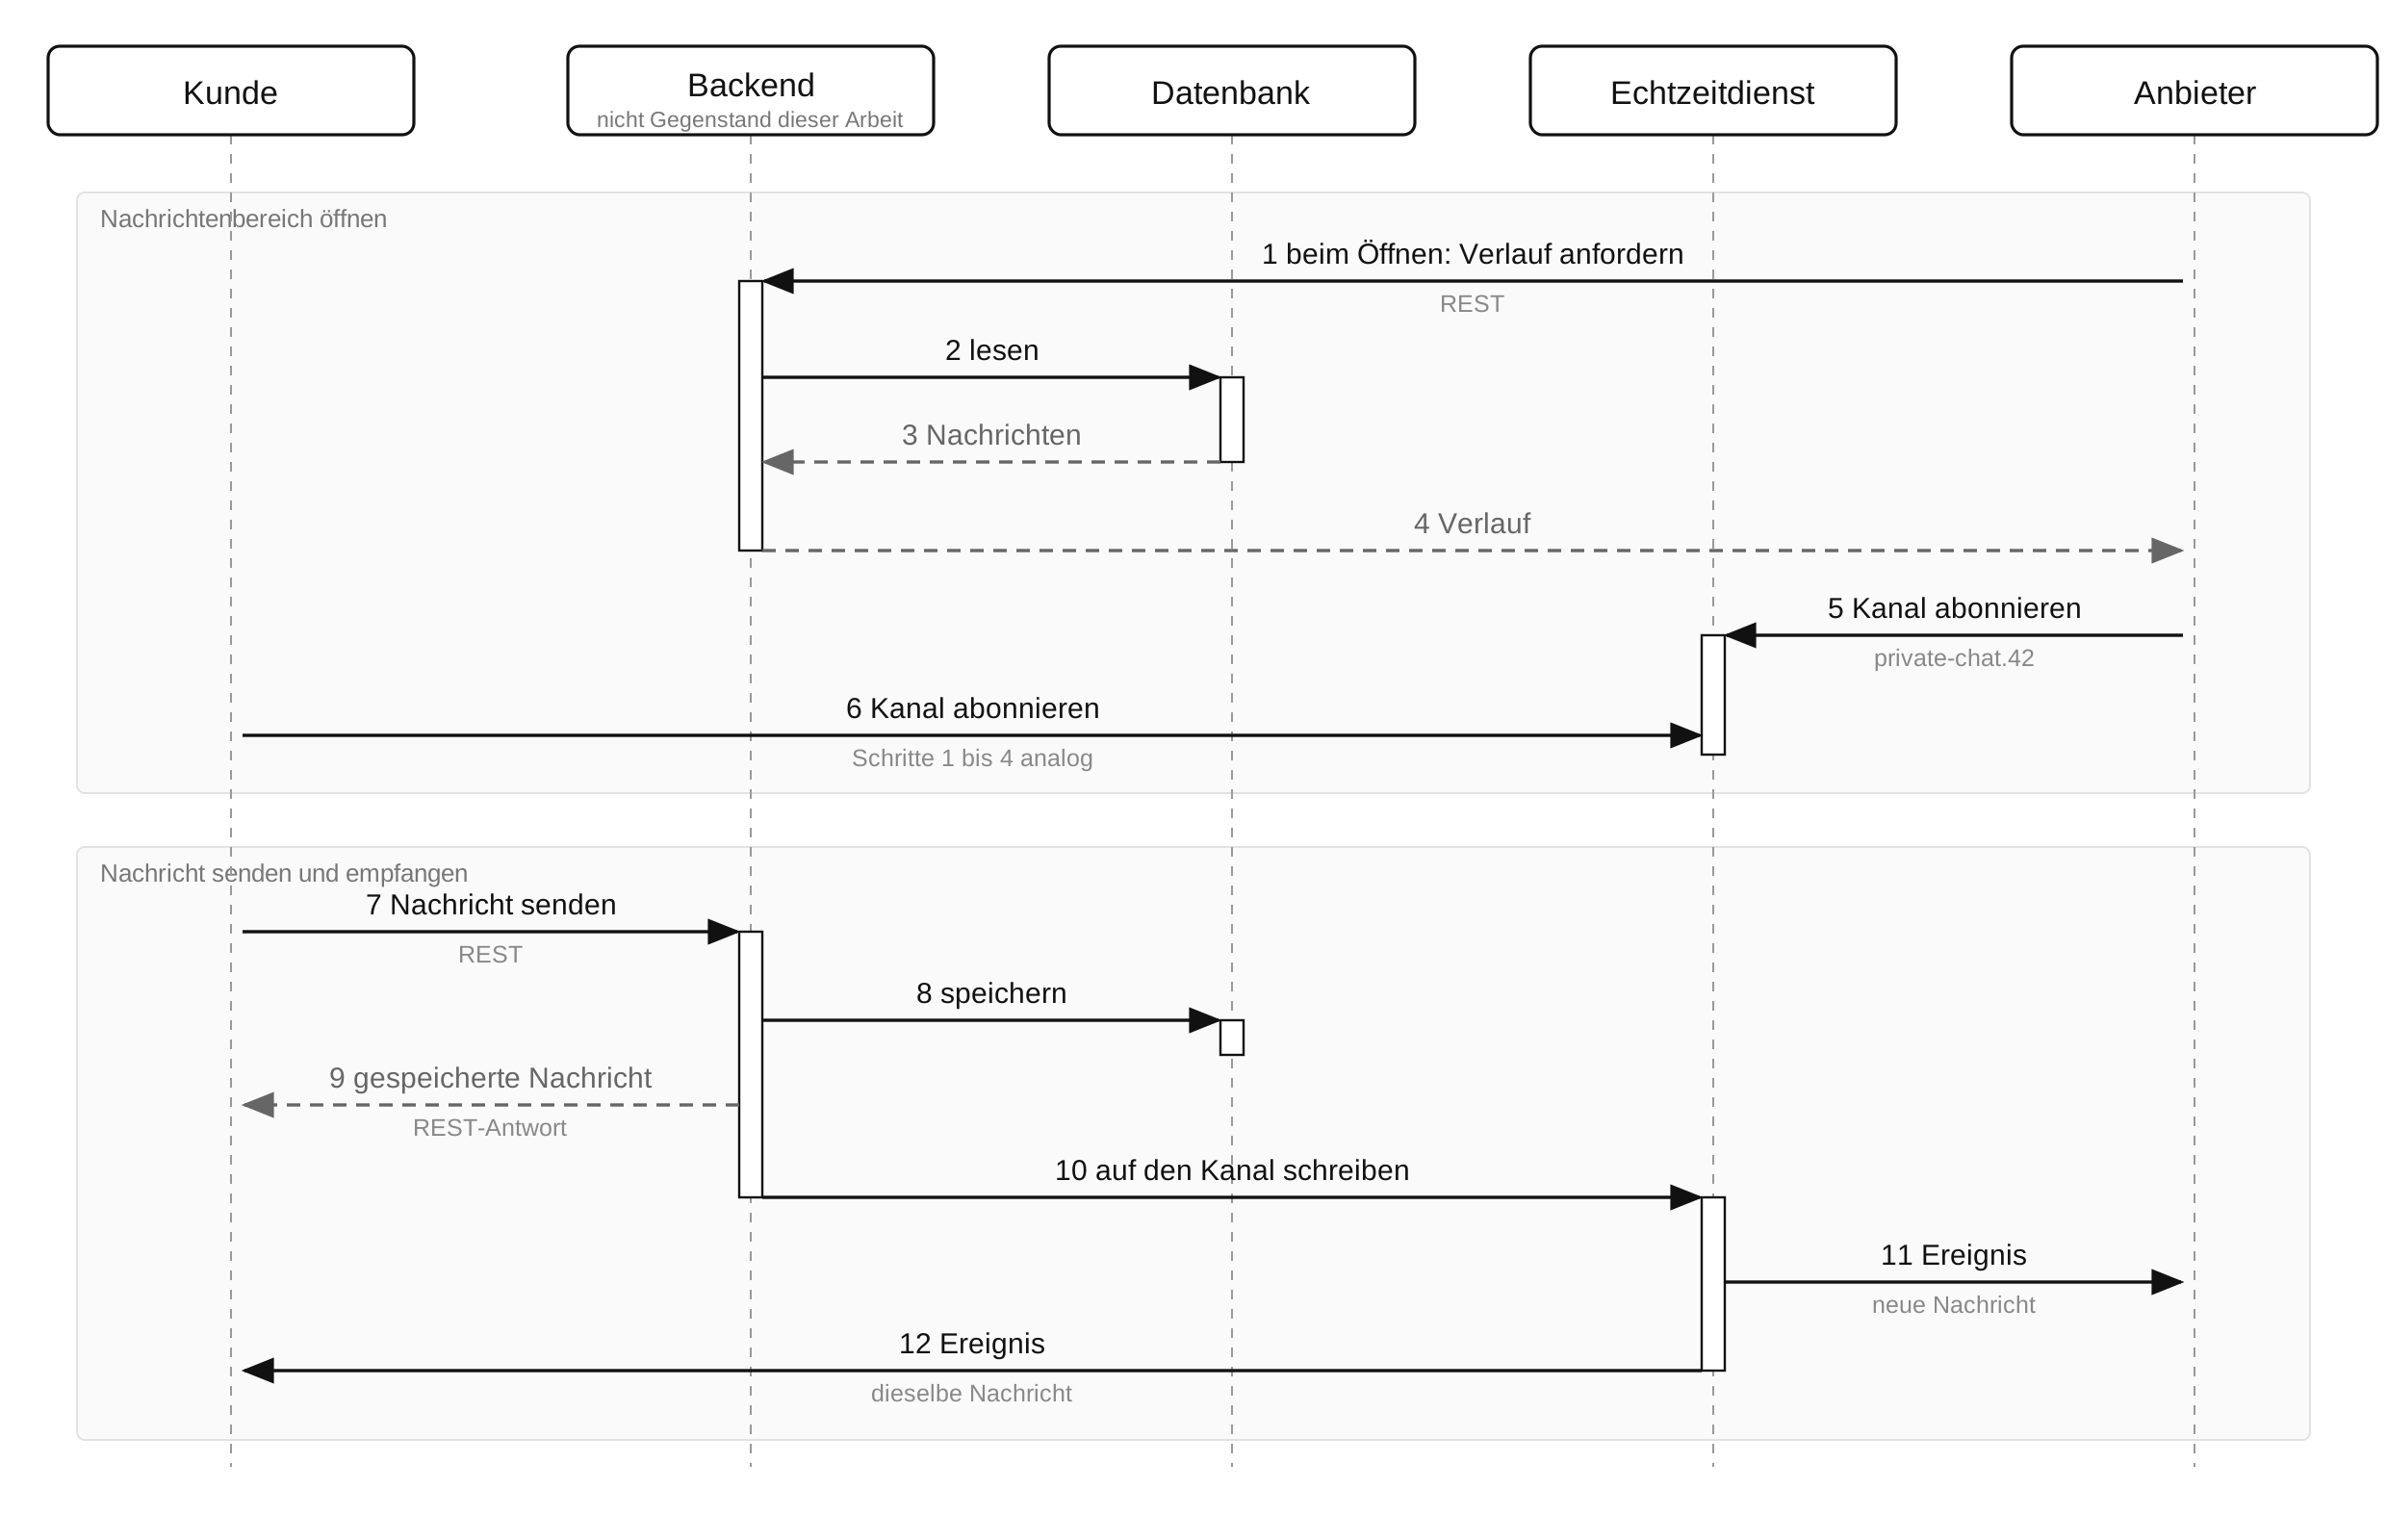
\includegraphics[width=\textwidth]{Bilder/abb_messaging.png}
\caption{Weg einer Nachricht zwischen Absender und Empfänger
(eigene Darstellung)}
\label{fig:messaging_ablauf}
\end{figure}
 
Neben der Unterhaltung selbst ist eine zweite Angabe in Echtzeit zu
übertragen: die Anzahl ungelesener Nachrichten. Sie wird in der
Kopfzeile angezeigt und muss sich auch dann aktualisieren, wenn der
Nutzer sich an einer beliebigen anderen Stelle der Anwendung
befindet. Da die Kanäle der Unterhaltungen dort nicht abonniert
sind, erhält jeder Nutzer zusätzlich einen auf ihn bezogenen Kanal,
über den ausschließlich dieser Zählerstand übermittelt wird.
 
Schließlich sieht der Entwurf drei Zustände je Nachricht vor:
gesendet, zugestellt und gelesen. Der Absender erkennt daran, ob
seine Nachricht angekommen ist und ob der Empfänger sie gelesen hat
(vgl. Abschnitt~\ref{subsec:gestaltungsprinzipien}).
    \chapter{Prototypische Umsetzung}
\label{chap:umsetzung}
Dieses Kapitel dokumentiert die Umsetzung des in
Kapitel~\ref{chap:konzept} beschriebenen Konzepts. Da eine
vollständige Wiedergabe des Quellcodes weder möglich noch
aufschlussreich wäre, folgt die Auswahl der Beispiele zwei
Gesichtspunkten: Sie zeigen entweder ein Muster, das an mehreren
Stellen der Anwendung wiederkehrt, oder eine Entscheidung, die sich
aus dem Code allein nicht erschließt. Die eingesetzten Werkzeuge
sind in Abschnitt~\ref{sec:technologieauswahl} beschrieben, die
Ordnerstruktur in Abschnitt~\ref{subsec:komponentenarchitektur}.
\section{Netzwerkkommunikation und Server-State}
\label{sec:impl_netzwerk}
 
Dieser Abschnitt beschreibt die konkrete Umsetzung des in
Abschnitt~\ref{subsec:netzwerk_konzept} vorgestellten
Drei-Schichten-Modells: einer zentralen \acs{HTTP}-Infrastruktur auf
Basis von Axios, einer feature-spezifischen \acs{API}-Schicht sowie
Query-Hooks auf Basis von TanStack Query, die den Verbindungszustand
für die aufrufenden Komponenten bereitstellen.
 
\subsection{HTTP-Client als Infrastruktur}
\label{subsec:impl_httpclient}
 
Die technische Infrastruktur der Netzwerkkommunikation wird durch
eine einzige, projektweit wiederverwendete Axios-Instanz
bereitgestellt \cite{axios_docs}. Listing~\ref{lst:http-client-infra}
zeigt deren vollständige Konfiguration. Die Instanz wird mit einer
festen Basis-Adresse sowie einheitlichen Standard-Headern
initialisiert; die Basis-Adresse lässt sich über eine
Umgebungsvariable überschreiben, sodass zwischen verschiedenen
Backend-Umgebungen gewechselt werden kann, ohne den Quellcode
anzupassen.
 
\begin{lstlisting}[caption={Zentrale Axios-Instanz mit
Request-Interceptor (http-client.ts)},
label={lst:http-client-infra}]
export const httpClient = axios.create({
  baseURL: resolveApiBaseUrl(),
  headers: {
    Accept: 'application/json',
    'Accept-Language': 'en',
    'Content-Type': 'application/json',
  },
})
 
httpClient.interceptors.request.use((config) => {
  const token = getAuthToken()
 
  if (token) {
    config.headers.Authorization = `Bearer ${token}`
  }
 
  return config
})
\end{lstlisting}
 
Über den Request-Interceptor wird der Authentifizierungstoken
automatisch an jede ausgehende Anfrage angehängt, sofern eine
gültige Sitzung vorliegt. Dadurch muss sich keine der
nachfolgend beschriebenen Feature-API-Funktionen selbst um die
Token-Übermittlung kümmern.
 
\subsection{Feature-API-Schicht}
\label{subsec:impl_featureapi}
 
Jeder Funktionsbereich definiert eigene \acs{API}-Funktionen, die
festlegen, welcher Endpunkt mit welcher \acs{HTTP}-Methode und welchen
Parametern angefragt wird. Diese Funktionen greifen ausschließlich
auf den in Abschnitt~\ref{subsec:impl_httpclient} beschriebenen
\texttt{httpClient} zurück und sind selbst frei von
Infrastruktur-Details. Listing~\ref{lst:feature-api-getme} zeigt
dies am Beispiel der Funktion \texttt{getMe()} aus dem
Account-Feature, die um optionale Parameter für die Einbindung einer
Zusammenfassung sowie eine Begrenzung der zurückgegebenen
Einträge ergänzt ist.
 
\begin{lstlisting}[caption={Feature-API-Funktion getMe
(account-api.ts)}, label={lst:feature-api-getme}]
export async function getMe(includeSummary = false, limit?: number) {
  const params = new URLSearchParams()
 
  if (includeSummary) {
    params.set('include', 'summary')
  }
 
  if (typeof limit === 'number') {
    params.set('limit', String(limit))
  }
 
  const queryString = params.toString()
  const path = queryString
    ? `${accountEndpoints.me}?${queryString}`
    : accountEndpoints.me
 
  const response = await httpClient.get<ApiSuccessResponse<MeResult>>(path)
 
  return response.data
}
\end{lstlisting}
 
Die Funktion baut die Query-Parameter abhängig von den übergebenen
Argumenten zusammen und gibt ausschließlich die Nutzdaten der
Antwort zurück. Sie enthält selbst keine Logik zur Behandlung von
Lade- oder Fehlerzuständen; diese Aufgabe übernimmt die in
Abschnitt~\ref{subsec:impl_tanstackquery} beschriebene Query-Hook-Schicht.
 
\subsection{Server-State mit TanStack Query}
\label{subsec:impl_tanstackquery}
 
Die oberste Schicht bilden Query-Hooks, die eine Feature-API-Funktion
mithilfe von TanStack Query kapseln und den aufrufenden Komponenten
den Zustand der Verbindung bereitstellen \cite{tanstack_query_docs}.
Listing~\ref{lst:use-me-query} zeigt den Hook
\texttt{useMeQuery}, der die zuvor beschriebene Funktion
\texttt{getMe()} verwendet.
 
\begin{lstlisting}[caption={Query-Hook useMeQuery
(use-me-query.ts)}, label={lst:use-me-query}]
export function useMeQuery(includeSummary = false, limit?: number, enabled = true) {
  return useQuery({
    queryKey: ['me', { includeSummary, limit }],
    queryFn: () => getMe(includeSummary, limit),
    enabled,
  })
}
\end{lstlisting}
 
Der \texttt{queryKey} setzt sich, wie in
Abschnitt~\ref{subsec:netzwerk_konzept} beschrieben, aus einer
festen Bezeichnung und den übergebenen Parametern zusammen und
identifiziert die Anfrage eindeutig im projektweiten Cache. Der
\texttt{enabled}-Parameter erlaubt es zusätzlich, die Ausführung
der Anfrage an eine Bedingung zu knüpfen, etwa das Vorhandensein
einer gültigen Sitzung.
 
Der Rückgabewert des Hooks stellt der aufrufenden Komponente die
Felder \texttt{data}, \texttt{isLoading} und \texttt{isError} zur
Verfügung, über die sich Ladeindikatoren und Fehlermeldungen
umsetzen lassen. In der Kontoübersicht wird dieses Muster
vereinfacht eingesetzt: Anstelle einer expliziten Auswertung von
\texttt{isLoading} und \texttt{isError} greift die Komponente auf
einen Fallback auf die bereits im Client gespeicherte Sitzung
zurück, sodass dem Nutzer zumindest der Benutzername angezeigt
werden kann, selbst wenn die Anfrage an das Backend noch nicht
abgeschlossen ist oder fehlschlägt. Für Ansichten ohne einen
solchen Fallback ist hingegen eine explizite Behandlung der von
TanStack Query bereitgestellten Zustände erforderlich.
 
Die Query-Hooks greifen dabei auf einen einmalig erzeugten,
zentralen Cache zurück, der über die gesamte Anwendung hinweg
geteilt wird und beim Anwendungsstart über einen Provider
bereitgestellt wird. Über die Zwischenspeicherung bereits
abgerufener Daten hinaus bietet TanStack Query den Mechanismus der
gezielten Invalidierung von Cache-Einträgen; dieser bildet die
alleinige, projektweit einheitliche Grundlage für die Aktualität
zwischengespeicherter Daten, anstelle einer zusätzlichen
Konfiguration fester Gültigkeitsdauern. Dieses Muster aus Query
Key, Cache und einheitlichen Verbindungszuständen kommt bei
sämtlichen weiteren Datenabrufen der Anwendung in gleicher Form
zum Einsatz und wird in den folgenden Abschnitten jeweils nur
noch kurz referenziert.
\section{Mehrsprachigkeit der Oberfläche}
\label{sec:impl_i18n}
 
Die Umsetzung des in
Abschnitt~\ref{subsec:mehrsprachigkeit_konzept} beschriebenen
Konzepts stützt sich auf \textit{i18next} mit der React-Anbindung
\textit{react-i18next} \cite{i18next_docs}. Die Oberflächentexte
liegen in zwei Modulen, je eines für Deutsch und Englisch; beide
enthalten dieselben Schlüssel und unterscheiden sich allein in den
Werten. Die Schlüssel sind nicht alphabetisch, sondern nach ihrem
Verwendungsbereich gruppiert -- etwa \texttt{header},
\texttt{cart} oder \texttt{checkout} --, wobei ein Bereich
\texttt{common} die mehrfach verwendeten Texte aufnimmt. Dieselbe
Bezeichnung kann dadurch in verschiedenen Bereichen einen eigenen
Wert tragen.
 
\begin{lstlisting}[caption={Auszug aus der deutschen Ressourcendatei (de.ts)}, label={lst:i18n-messages}]
const de = {
  common: {
    cart: 'Warenkorb',
    noDescriptionYet: 'Noch keine Beschreibung.',
  },
  catalog: {
    bySeller: 'von {{name}}',
  },
  checkout: {
    successTitle: 'Checkout erfolgreich',
    paymentConfirmed: 'Zahlung bestaetigt',
  },
}
\end{lstlisting}
 
Der Eintrag \texttt{bySeller} zeigt die Behandlung veränderlicher
Bestandteile: Der Platzhalter wird beim Anzeigen ersetzt, sodass der
Satzbau in der Ressourcendatei verbleibt und nicht im Quelltext
zusammengesetzt wird -- was nötig ist, da die Stellung eines
eingesetzten Wortes von Sprache zu Sprache verschieden ist.
 
Die Konfiguration erfolgt an einer Stelle und wird beim Start noch
vor der ersten Darstellung ausgeführt. Sie legt die Ressourcen, die
Rückfallsprache und die Reihenfolge fest, in der die Sprache
ermittelt wird: zunächst der gespeicherte Wert, andernfalls die
Spracheinstellung des Browsers. Die Wahl wird im
\texttt{localStorage} abgelegt, derselben Ablage wie die Sitzung
(vgl. Abschnitt~\ref{subsec:impl_token_session}), und ist in einem
eigenen Hook gekapselt; der Umschalter greift ausschließlich darauf
zu und kennt weder die Bibliothek noch die Art der Speicherung.
 
Die Inhalte aus dem Backend werden dagegen nicht übersetzt, sondern
angefordert: Der in Abschnitt~\ref{subsec:impl_httpclient}
beschriebene zentrale \acs{HTTP}-Client führt bei jeder Anfrage einen
Header mit der gewählten Sprache mit. Der Wert wird im Interceptor
gesetzt und nicht bei der Erzeugung der Instanz, da er sonst auf dem
Stand des Anwendungsstarts bliebe. Eine einzige Stelle genügt damit,
um die Sprachwahl auf sämtliche Inhalte wirken zu lassen.
 
Sichtbar wird dies gegenwärtig gleichwohl nicht: Die
Erfassungsformulare sehen Englisch und Arabisch vor (vgl.
Abschnitt~\ref{subsec:impl_dienstleistungsverwaltung}), sodass keine
deutsche Fassung der Inhalte entsteht und das Backend auf die
deutsche Anforderung mit der englischen antwortet. Die Übertragung
der Sprachwahl ist im Frontend somit vollständig umgesetzt, wirkt
sich auf die Inhalte jedoch erst aus, sobald das Datenmodell eine
deutsche Fassung vorsieht.
\section{Authentifizierung und Onboarding}
\label{sec:impl_auth}

\subsection{Registrierung und Login}
\label{subsec:impl_registrierung_login}
 
Entsprechend dem Konzept aus
Abschnitt~\ref{subsec:auth-onboarding} ist die Registrierung als
eigene Seite umgesetzt, der Login als Dialog. Dieser überlagert die
aufrufende Seite, ohne sie zu ersetzen, sodass der Nutzer nach der
Anmeldung ohne Umweg an die Stelle zurückkehrt, an der er sich befand.
 
\begin{figure}[H]
\centering
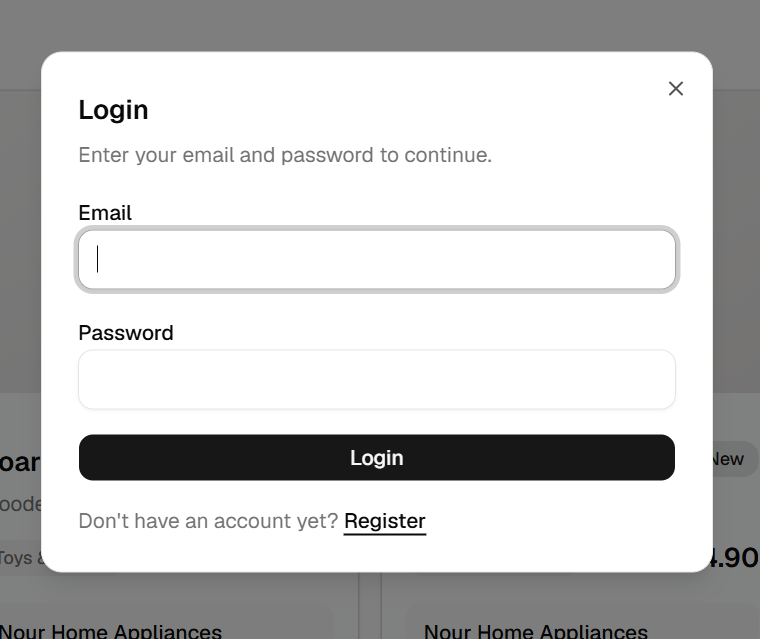
\includegraphics[width=0.7\textwidth]{Bilder/screenshot_login_dialog.png}
\caption{Login-Dialog}
\label{fig:login_dialog}
\end{figure}
 
Beide Formulare werden über \texttt{react-hook-form} in Verbindung
mit einem Zod-Schema validiert (vgl.
Abschnitt~\ref{subsec:formulare-validierung}). Das Schema der
Registrierung prüft dabei nicht nur einzelne Felder, sondern auch
deren Verhältnis zueinander.
 
\begin{lstlisting}[caption={Validierungsschema der Registrierung (register-schema.ts)}, label={lst:register-schema}]
export const registerSchema = z
  .object({
    name: z
      .string()
      .trim()
      .min(1, 'Name is required.')
      .max(255, 'Name must be 255 characters or fewer.'),
    age: z.preprocess(
      (value) =>
        value === '' || value === undefined || Number.isNaN(value) ? null : value,
      z
        .number({ error: 'Enter a valid age.' })
        .int()
        .min(12, 'Age must be at least 12.')
        .max(100, 'Age must be 100 or less.')
        .nullable(),
    ),
    email: z
      .string()
      .trim()
      .min(1, 'Email is required.')
      .email('Enter a valid email address.'),
    phone: z.preprocess(emptyToUndefined, z.string().optional()),
    password: z.string().min(6, 'Password must be at least 6 characters.'),
    password_confirmation: z.string().min(1, 'Please confirm your password.'),
  })
  .superRefine((values, context) => {
    if (values.password !== values.password_confirmation) {
      context.addIssue({
        code: 'custom',
        message: 'Passwords do not match.',
        path: ['password_confirmation'],
      })
    }
  })
\end{lstlisting}
 
Die einzelnen Feldregeln lassen sich unabhängig voneinander prüfen.
Die Übereinstimmung von Passwort und Bestätigung dagegen nicht, da
sie zwei Werte zugleich betrifft; sie wird deshalb über
\texttt{superRefine} auf der Ebene des gesamten Objekts geprüft und
über die Angabe eines Pfades dem Bestätigungsfeld zugeordnet. Eine
eigene Längenregel benötigt das Bestätigungsfeld dadurch nicht: Da
es dem Passwort entsprechen muss und dieses mindestens sechs Zeichen
umfasst, ergibt sich seine Länge aus der Übereinstimmung.
 
Die beiden freiwilligen Felder werden vor der Prüfung aufbereitet.
Beim Telefonfeld ersetzt eine Hilfsfunktion eine leer gebliebene
Eingabe durch \texttt{undefined}, beim Altersfeld durch
\texttt{null}, sodass ein nicht ausgefülltes Feld nicht als leerer
Text an das Backend gelangt. Bei den Pflichtfeldern unterbleibt
diese Aufbereitung, und es genügt \texttt{trim}: Dort ist eine leere
Eingabe gerade der Fehlerfall und darf nicht in einen fehlenden Wert
umgedeutet werden, weil die zugehörige Regel sonst nicht mehr
greifen könnte.
 
\begin{figure}[H]
\centering
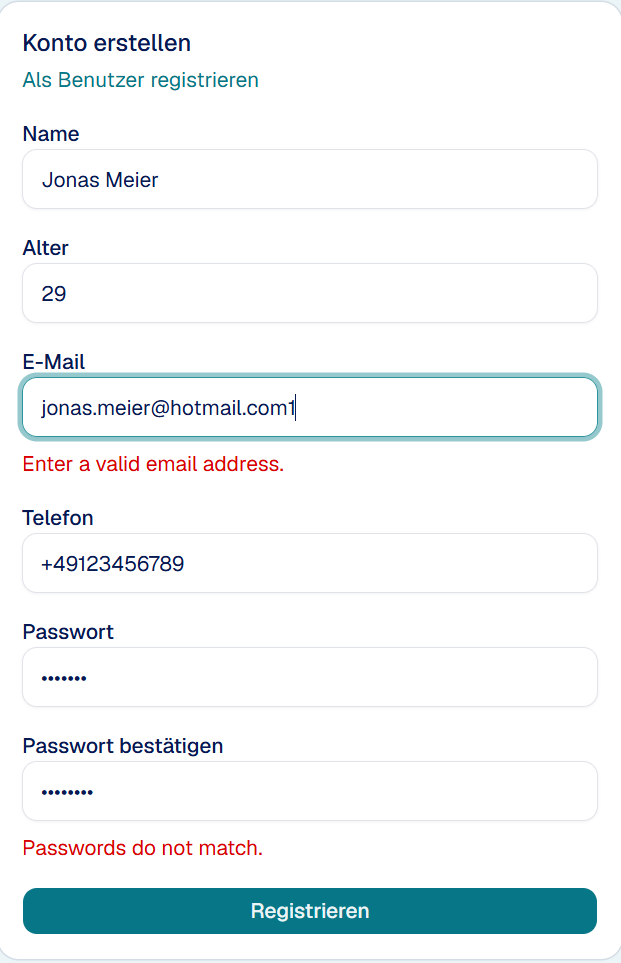
\includegraphics[width=0.55\textwidth]{Bilder/screenshot_registrierung_fehler.png}
\caption{Registrierungsformular mit einem Formatfehler im
E-Mail-Feld und einer feldübergreifenden Abweichung zwischen Passwort
und Bestätigung}
\label{fig:registrierung_fehler}
\end{figure}
 
Die Meldungen stehen unmittelbar unter dem betroffenen Feld,
benennen die verletzte Regel und bleiben stehen, bis die Eingabe
korrigiert ist; die übrigen Eingaben bleiben erhalten, sodass ein
fehlgeschlagener Versuch nicht zum erneuten Ausfüllen des gesamten
Formulars zwingt (vgl.
Abschnitt~\ref{subsec:gestaltungsprinzipien}).
 
Nicht alle Prüfungen können im Frontend stattfinden: Ob eine
E-Mail-Adresse bereits vergeben ist oder ein Passwort dem
hinterlegten entspricht, kann nur das Backend beantworten.
Serverseitig gemeldete Fehler werden deshalb demselben Feld
zugeordnet und in derselben Form dargestellt wie clientseitige;
nicht zuordenbare Fehler erscheinen als allgemeine Meldung über dem
Formular.
 
Verläuft die Anfrage erfolgreich, wird die Sitzung im
Authentifizierungszustand gespeichert; beim Login schließt sich der
Dialog, bei der Registrierung erfolgt eine Weiterleitung auf die
Startseite.

\subsection{Token-Verwaltung und Session-Handling}
\label{subsec:impl_token_session}
Die Session der Anwendung ist als eigenes Modell definiert, das
Zugriffstoken, Nutzerdaten und die zugewiesenen Rollen als Liste
enthält, da ein Nutzer mehrere Rollen gleichzeitig besitzen kann. Sie
wird über einen zentralen Zustand-Store reaktiv bereitgestellt und im
\texttt{localStorage} des Browsers gespeichert, um den Anmeldestatus
über Neuladen und erneute Besuche hinweg zu erhalten.
Listing~\ref{lst:auth-store-state} zeigt die Struktur dieses Stores
sowie dessen Erzeugung über die \texttt{create}-Funktion der
Bibliothek Zustand.
 
\begin{lstlisting}[caption={Struktur und Erzeugung des Auth-Stores (auth-store.ts)}, label={lst:auth-store-state}]
import { create } from 'zustand'
 
interface AuthStoreState {
  session: AuthSession | null
  isAuthenticated: boolean
  isBootstrapping: boolean
  setSession: (session: AuthSession) => void
  setBootstrapping: (isBootstrapping: boolean) => void
  syncVerifiedUser: (user: User) => void
  clearSession: () => void
}
 
export const useAuthStore = create<AuthStoreState>((set, get) => ({
  // ...
}))
\end{lstlisting}
 
Ein gespeicherter Token wird nicht ungeprüft als gültig angenommen:
Eine Bootstrap-Komponente validiert ihn aktiv beim Backend über
\texttt{useMeQuery} (vgl.
Abschnitt~\ref{subsec:impl_tanstackquery}). Liefert diese Anfrage
einen Fehler, gilt der Token als ungültig und die Session wird über
den Store verworfen; liefert sie hingegen aktualisierte Nutzerdaten,
werden diese im Store synchronisiert, sodass lokal gespeicherte und
serverseitig bestätigte Daten konsistent bleiben. Liegt noch keine
Antwort vor, wird zunächst die lokal gespeicherte Session verwendet,
damit die Oberfläche sofort angezeigt werden kann. Auf dieser
Grundlage entscheidet eine geschützte Routenkomponente, ob der
Anmeldestatus noch ermittelt wird, der Nutzer zur Startseite
weitergeleitet oder der geschützte Inhalt angezeigt wird.

\subsection{Rollen-Upgrade-Antrag}
\label{subsec:impl_rollen_upgrade}

Wie in Abschnitt~\ref{subsec:auth-onboarding} beschrieben, kann
ein Nutzer über die Kontoübersicht einen Antrag auf die Rolle
	extit{Seller} oder 	extit{ServiceProvider} stellen. Zusätzlich zu den Basisdaten
werden dabei projektspezifische Angaben wie Name und Kontaktdaten
des Geschäfts sowie ein Nachweisdokument erfasst, anhand derer ein
Administrator über den Antrag entscheidet. Bis zur Entscheidung
bleibt der Nutzer uneingeschränkt in seiner Rolle als 	extit{Customer}
aktiv; nach einer Genehmigung stehen ihm zusätzliche,
rollenspezifische Seiten zur Verfügung.

% TODO (Roudy): Hier Screenshot der Kontouebersicht vor und nach
% der Genehmigung nebeneinander einfuegen (vgl. Meeting vom
% 12.07.2026), kein Code, kein Diagramm.
\section{Katalog und Produktseiten}
\label{sec:impl_katalog}

\subsection{Produktlisting: Karten, Paginierung}
\label{subsec:impl_produktlisting}

Dieser Abschnitt beschreibt die Umsetzung der in
Abschnitt~\ref{subsec:katalog_konzept} vorgestellten Startseite
sowie das wiederverwendbare Kartenprinzip, das dort zum Einsatz
kommt. Die Startseite ruft ihre Daten über eine einzelne, an den
Endpunkt \texttt{/api/home} gerichtete Anfrage ab, die Produkte
und Dienstleistungen gemeinsam liefert. Der Aufbau der
Anfragefunktion und des zugehörigen Query-Hooks folgt dabei
demselben Prinzip, das bereits in
Abschnitt~\ref{sec:impl_netzwerk} eingeführt wurde. Während des
Ladens wird ein Platzhalter-Raster angezeigt, im Fehlerfall eine
Fehlermeldung; im Unterschied zur Kontoübersicht (vgl.
Abschnitt~\ref{subsec:impl_tanstackquery}) steht hier keine
lokal gespeicherte Alternative zur Verfügung, sodass diese
Zustände explizit behandelt werden.

Sowohl der Produkt- als auch der Dienstleistungsbereich der
Startseite nutzen dieselbe wiederverwendbare
Vorschau-Komponente, die Titel, Leer-Zustand-Nachricht und den
eigentlichen Karteninhalt entgegennimmt. Jedes Produkt wird über
eine Karte dargestellt, die den vom Backend gelieferten,
unvollständigen Bildpfad um die Basis-Adresse ergänzt, den Preis
über die integrierte \texttt{Intl.NumberFormat}-Schnittstelle
formatiert und bei kürzlich hinzugefügten Produkten eine
entsprechende Kennzeichnung anzeigt.

Auf der Katalogseite für Produkte lassen sich die angezeigten
Einträge zusätzlich nach Kategorie filtern und seitenweise
durchblättern; Seite und Kategorie werden als Suchparameter in
der \acs{URL} abgebildet, sodass sich ein bestimmter Ausschnitt des
Katalogs verlinken lässt. Da diese Parameter Teil des Query Keys
sind (vgl. Abschnitt~\ref{subsec:impl_tanstackquery}), führt
sowohl ein Seitenwechsel als auch eine geänderte Kategorie zu
einer neuen Anfrage an das Backend.

\subsection{Produktdetailseite \& Dienstleistungsdetailseite}
\label{subsec:impl_produktdetail}

Der Aufruf einer Produktkarte führt, wie in
Abschnitt~\ref{subsec:katalog_konzept} beschrieben, auf die
zugehörige Detailseite; die Produkt-ID wird dabei als validierter
Routenparameter übergeben (vgl.
Abschnitt~\ref{subsec:routing-konzept}) und an den zugehörigen
Query-Hook weitergereicht. Die Seite unterscheidet vier
Zustände: eine ungültige Produkt-ID, den Ladezustand, einen
Fehler bei der Anfrage sowie den Fall, dass kein Produkt zu der
angefragten ID existiert. Liegen die Produktdaten vor, werden sie
in einer Bildergalerie, die auf dieselbe Bildpfad-Auflösung
zurückgreift wie die Produktkarte, sowie einer Übersicht mit
Preis, Kategorie und Verkäuferinformationen dargestellt.

% ----------------------------------------------------------------
% TODO (Roudy): Screenshot der Startseite mit den
% Vorschau-Karten (Produkte und Dienstleistungen,
% inkl. "New"-Kennzeichnung).

% TODO (Roudy): Screenshot der Produkt-Katalogseite mit
% Kategoriefilter und Paginierung (Seite/Kategorie in der URL
% sichtbar, z. B. /products?page=2&category=3).

% ----------------------------------------------------------------
\subsection{Terminauswahl auf der Dienstleistungsseite}
\label{subsec:impl_terminauswahl}
 
Die in Abschnitt~\ref{subsec:buchung_konzept} beschriebene Auswahl
ist als eigenständige, wiederverwendbare Komponente umgesetzt und auf
der Dienstleistungs-Detailseite eingebunden. Sie durchläuft drei
Zustände.
 
Im Ausgangszustand zeigt sie einen Monatskalender und die Zeitzone
des Anbieters. Welche Zeitfenster ein Tag enthält, ergibt sich erst
aus der Antwort des Backends; die Schaltfläche zur Übernahme in den
Warenkorb bleibt zunächst deaktiviert. Jeder Tag ist anwählbar, auch
ein solcher ohne Arbeitszeit -- an Stelle der Liste erscheint dann
der Hinweis, dass für dieses Datum keine Zeitfenster verfügbar sind
(vgl. Abschnitt~\ref{subsec:verkaeufer_dashboard_konzept}).
 
Mit der Wahl eines Tages wird dessen Zeitfensterliste abgerufen. Die
Fenster werden nach Tageszeit in Vormittag, Nachmittag und Abend
gruppiert; jedes trägt seinen Zeitraum und die verbleibende
Kapazität. Erst mit der Wahl eines Fensters erscheint eine
Zusammenfassung der Buchung, und die Schaltfläche wird aktiv.
 
\begin{figure}[H]
\centering
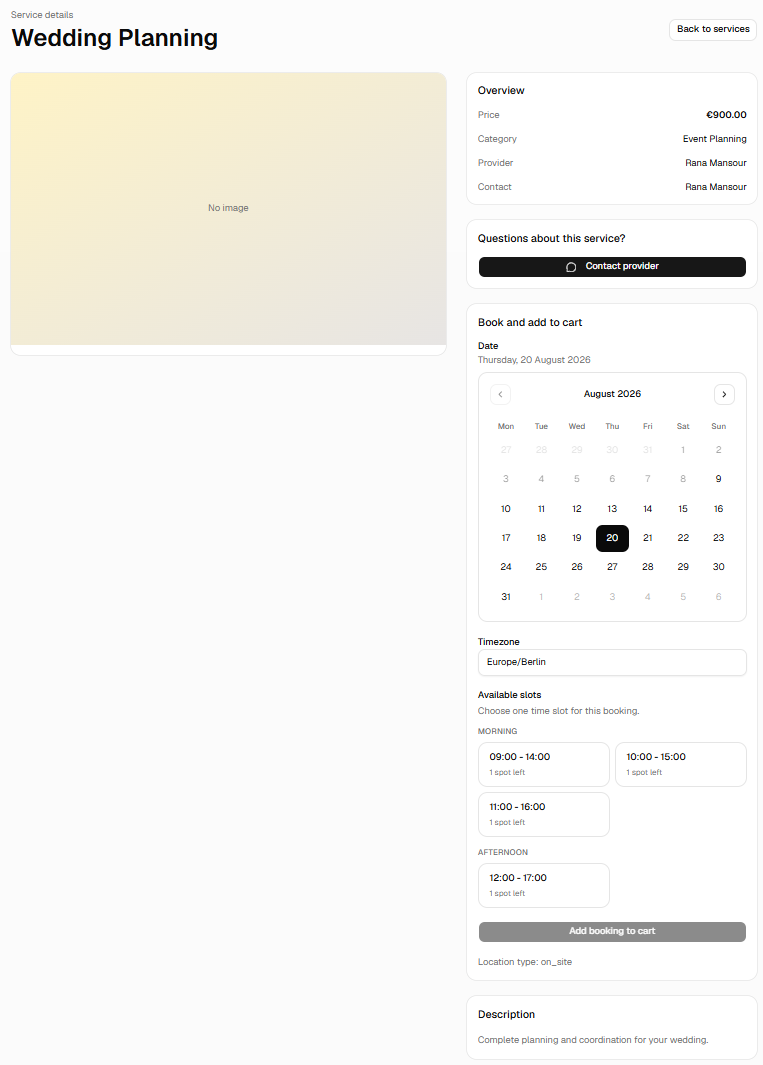
\includegraphics[width=0.60\textwidth]{Bilder/screenshot_buchung_auswahl.png}
\caption{Terminauswahl nach Wahl von Tag und Zeitfenster}
\label{fig:buchung_auswahl}
\end{figure}
 
Am Zeitraster der Fenster ist die Wirkung der Buchungsregeln
ablesbar: Bei einer Dauer von drei Stunden und einem Raster von
dreißig Minuten beginnen aufeinanderfolgende Fenster jeweils eine
halbe Stunde später und überlappen sich damit. Sie schließen einander
nicht aus, solange die Kapazität nicht erschöpft ist.
 
Die Übernahme in den Warenkorb erzeugt eine Position, die neben
Titel, Preis und Kategorie zusätzlich Beginn, Ende, Zeitzone und Ort
der Leistungserbringung trägt (vgl.
Abschnitt~\ref{subsec:impl_warenkorb}).


\section{Warenkorb, Checkout und Zahlung}
\label{sec:impl_checkout}


\subsection{Warenkorb-UI: Produkte und Buchungen kombiniert}
\label{subsec:impl_warenkorb}

Der Warenkorb ist als eigener Zustand-Store umgesetzt, getrennt vom
Auth- und vom \acs{UI}-Store (vgl.
Abschnitt~\ref{subsec:state-management-konzept}). Seine Persistenz
übernimmt die \texttt{persist}-Middleware von Zustand, die den Inhalt
unter dem Schlüssel \texttt{bazario-cart} im \texttt{localStorage}
ablegt \cite{zustand_docs}. Gespeichert wird dabei nicht der gesamte
Store, sondern über \texttt{partialize} nur der übertragbare Teil:
die Positionen, die Währung und die Zuordnung zum Besitzer. Die
abgeleiteten Funktionen für Zwischensumme und Positionszahl bleiben
ausgeschlossen, da sie sich aus den Positionen jederzeit neu
berechnen lassen.
 
Die beiden Positionstypen werden beim Hinzufügen unterschiedlich
behandelt. Ein Produkt wird über seine Kennung erkannt; ist es
bereits enthalten, erhöht sich lediglich dessen Menge. Eine
Dienstleistungsbuchung besitzt dagegen keine Menge, sondern einen
Termin. Zwei Buchungen gelten deshalb nur dann als dieselbe, wenn
sechs Angaben übereinstimmen: die Dienstleistung, Beginn, Ende,
Zeitzone, die Art des Ortes und dessen nähere Bestimmung. Trifft das
zu, bleibt der Warenkorb unverändert; dieselbe Dienstleistung zu
einem anderen Termin ist dagegen eine eigene Position.
 
Ein dritter Punkt ergibt sich daraus, dass der Warenkorb im Browser
verbleibt und nicht am Konto hängt. Er führt deshalb mit, wem er
gehört, und gleicht diese Zuordnung bei jeder Änderung des
Anmeldestatus ab: Meldet sich ein zuvor nicht angemeldeter Nutzer
an, bleiben seine Positionen erhalten und werden ihm zugeordnet.
Wechselt dagegen der angemeldete Nutzer, wird der Warenkorb geleert.
Andernfalls fände ein Nutzer, der sich am selben Gerät anmeldet, die
Positionen seines Vorgängers vor.
\begin{figure}[H]
\centering
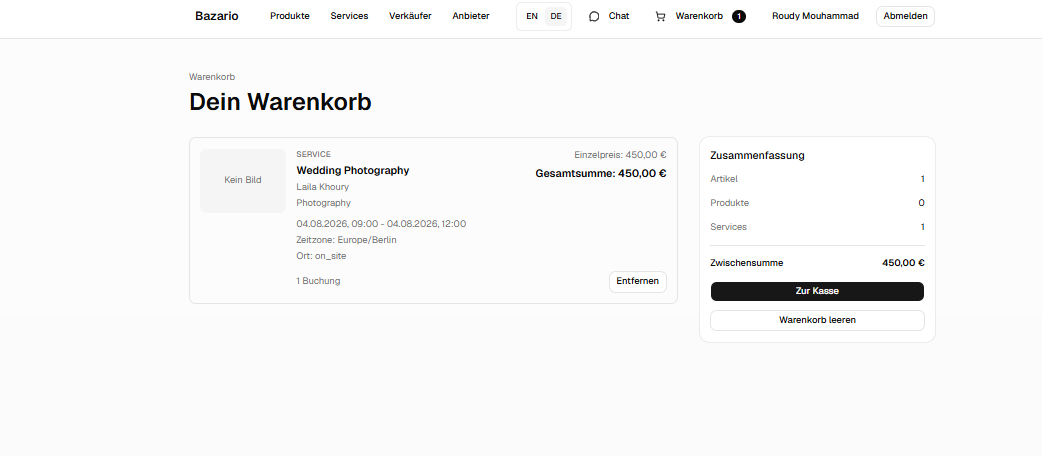
\includegraphics[width=\textwidth]{Bilder/screenshot_warenkorb_buchung.png}
\caption{Dienstleistungsbuchung als Position im Warenkorb}
\label{fig:warenkorb_buchung}
\end{figure}

\subsection{Stripe-Integration im Frontend}
\label{subsec:impl_stripe}
 
Die Umsetzung des in Abschnitt~\ref{subsec:warenkorb_konzept}
beschriebenen Konzepts verteilt sich auf zwei Stellen im Frontend:
das Auslösen des Checkouts im Warenkorb und die Verarbeitung des
Ergebnisses auf den beiden Rückleitungsseiten. Dazwischen liegt eine
Folge von Schritten, an denen Frontend, Backend und Zahlungsdienst
beteiligt sind.
 
\begin{figure}[H]
\centering
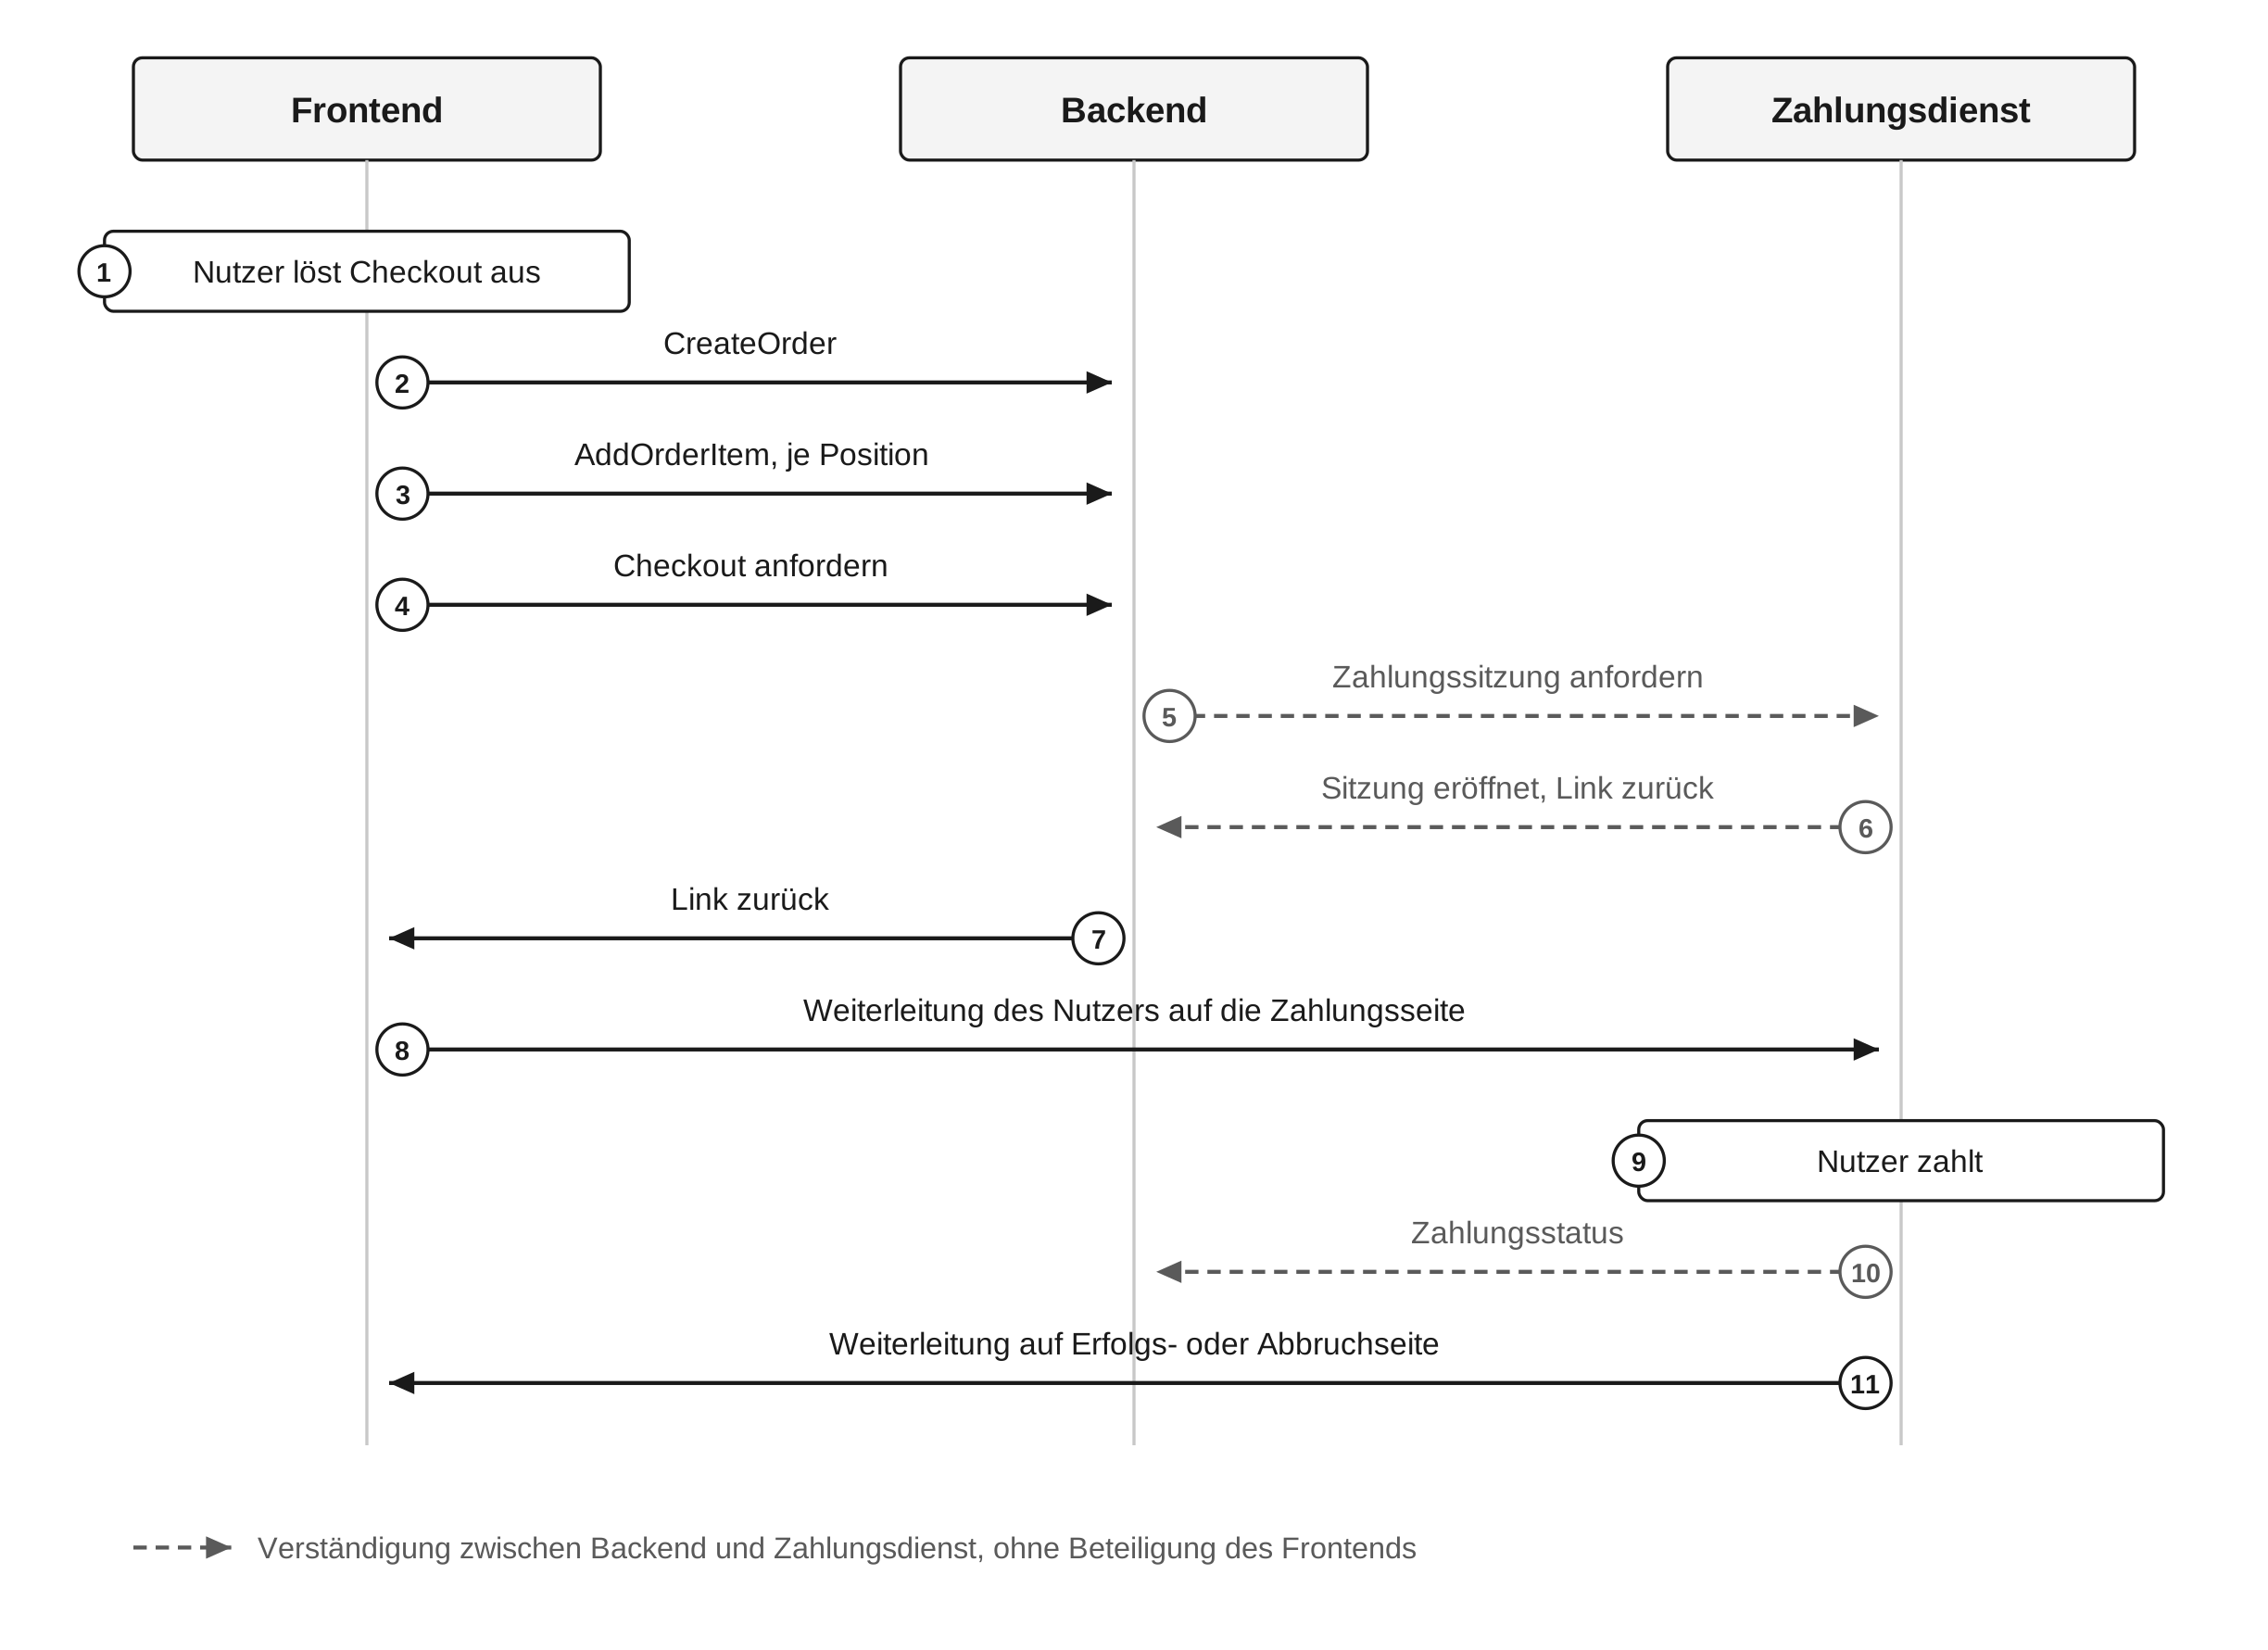
\includegraphics[width=0.8\textwidth]{Bilder/abb_checkout_ablauf.png}
\caption{Ablauf der Zahlung vom Auslösen des Checkouts bis zur
Rückleitung in die Anwendung}
\label{fig:checkout_ablauf}
\end{figure}
 
Vom Frontend gehen dabei nur drei Anfragen aus: das Anlegen des
Auftrags, das Hinzufügen der Positionen und das Anfordern der
Zahlungssitzung. Die Verständigung mit dem Zahlungsdienst erfolgt
vollständig im Backend.
 
Ausgelöst wird der Vorgang über die Schaltfläche in der
Warenkorbübersicht. Ist der Nutzer nicht angemeldet, öffnet die
Funktion über den \acs{UI}-Store den Anmeldedialog und bricht ab; der
Warenkorb bleibt dabei unverändert. Andernfalls läuft die
Checkout-Operation an, die als Mutation umgesetzt ist, da sie den
Datenbestand auf dem Server verändert (vgl.
Abschnitt~\ref{subsec:impl_tanstackquery}). Sie durchläuft drei
Schritte: Zunächst wird über die Feature-\acs{API} ein Auftrag
angelegt, dessen Kennung das Backend zurückgibt. Anschließend wird
für jede Position des Warenkorbs eine weitere Anfrage gestellt, die
sie diesem Auftrag zuordnet. Zuletzt wird die Zahlungssitzung
angefordert; das Backend liefert die Adresse der Zahlungsseite
zurück, auf die das Frontend den Browser weiterleitet.
 
\begin{figure}[H]
\centering
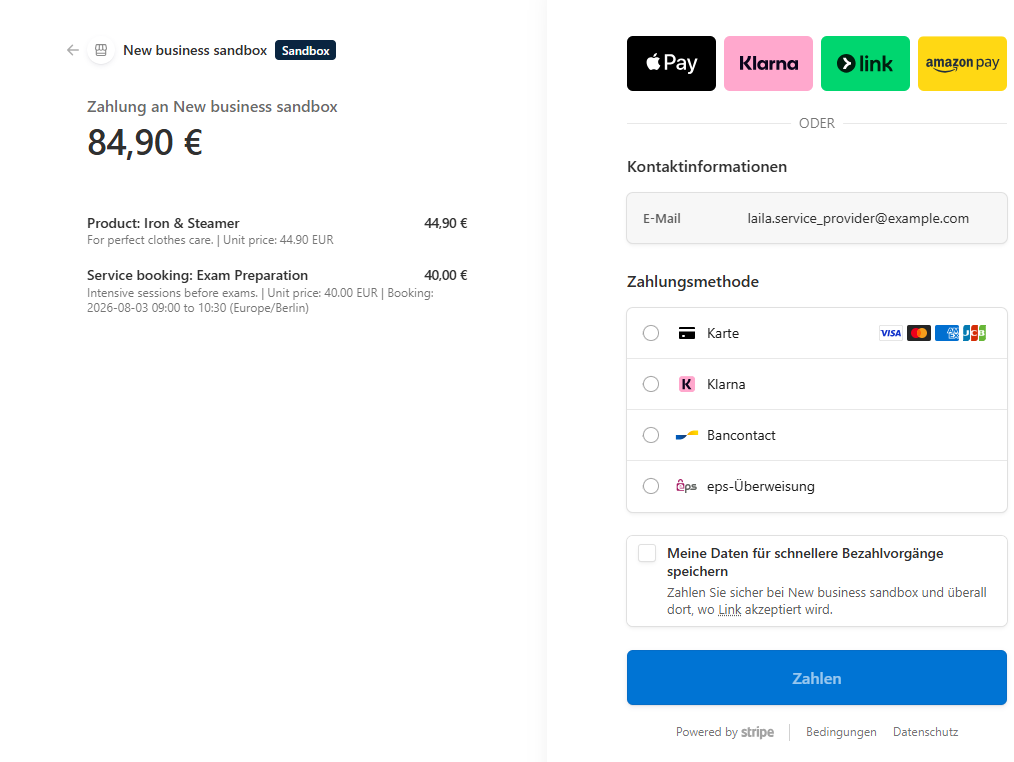
\includegraphics[width=0.7\textwidth]{Bilder/screenshot_stripe_zahlungsseite.png}
\caption{Von Stripe bereitgestellte Zahlungsseite, auf die das
Frontend nach dem Auslösen des Checkouts weiterleitet}
\label{fig:stripe_zahlungsseite}
\end{figure}
 
Die Aufbereitung der einzelnen Position ist in eine eigene Funktion
ausgelagert, da sich die zu übertragenden Angaben je nach
Positionstyp unterscheiden: Für ein Produkt genügen Kennung und
Menge, während eine Dienstleistungsbuchung zusätzlich den gewählten
Termin enthält. Die Fallunterscheidung liegt damit nicht in der
Mutation, die dadurch auf ihre drei Schritte beschränkt bleibt.
 
Nach Abschluss der Zahlung führt der Zahlungsdienst den Nutzer auf
eine der beiden Rückleitungsseiten zurück. Die Erfolgsseite ruft die
Auftragsdaten ab und zeigt Auftragsnummer, Status und Betrag an;
darunter bietet sie zwei Wege in die Übersichten an, getrennt nach
Bestellungen und Buchungen, da ein Auftrag beide Positionstypen
enthalten kann (vgl.
Abschnitt~\ref{subsec:gestaltungsprinzipien}).
 
\begin{figure}[H]
\centering
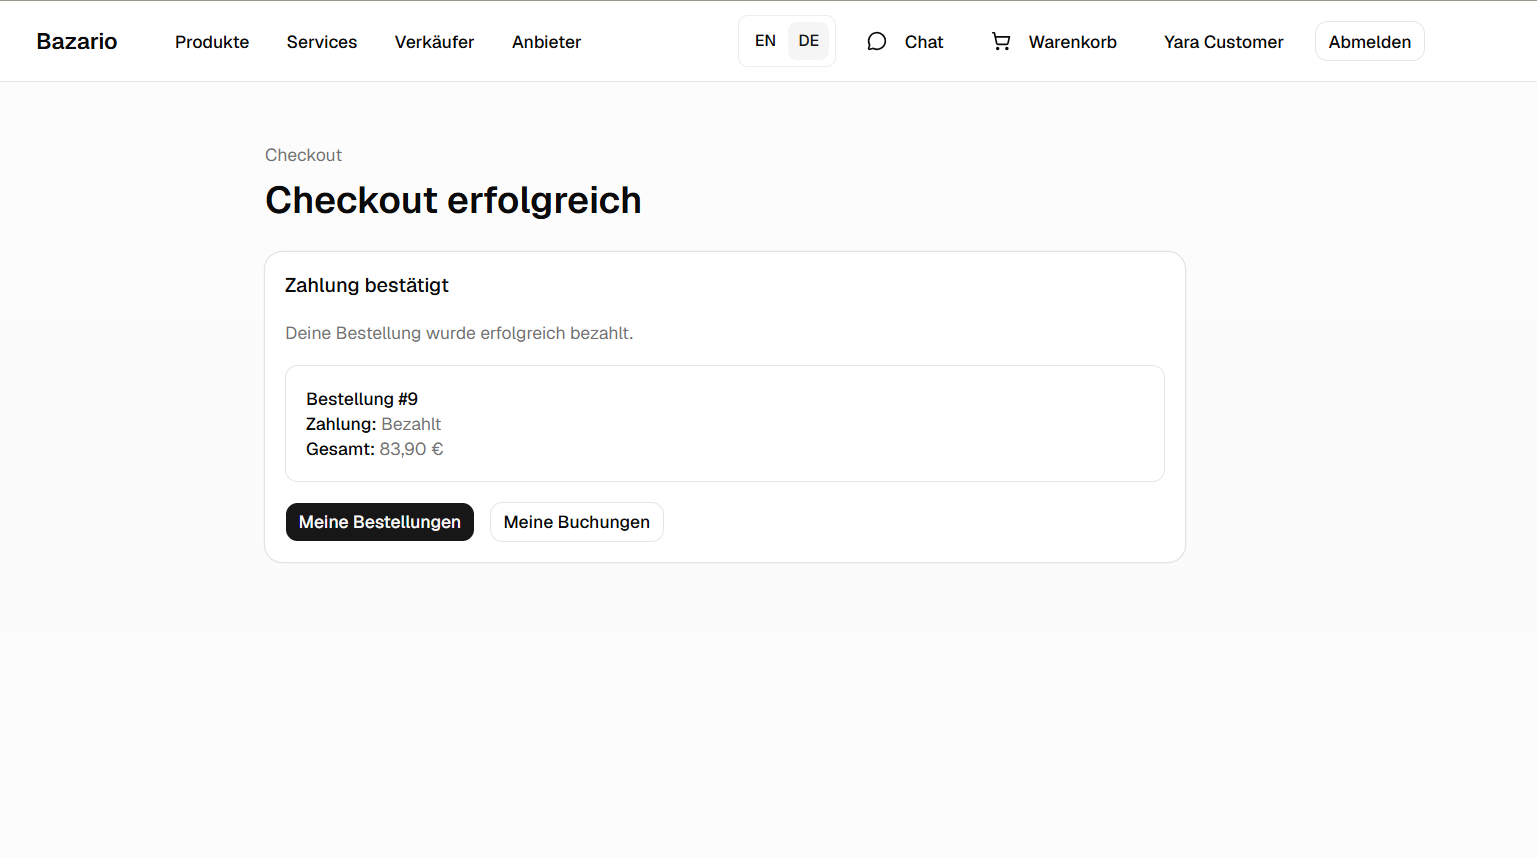
\includegraphics[width=0.85\textwidth]{Bilder/screenshot_checkout_success.png}
\caption{Bestätigungsseite nach erfolgreicher Zahlung}
\label{fig:checkout_success}
\end{figure}
 
Vor der Darstellung führt die Seite eine Folge von Nebenwirkungen
aus, die in einem Effekt gekapselt sind. Der Effekt prüft zunächst,
ob die Zahlung tatsächlich erfolgt ist, und bricht andernfalls ab.
Erst danach wird der Warenkorb geleert -- nicht schon beim Auslösen
des Checkouts, da die Zahlung bis zuletzt scheitern oder abgebrochen
werden kann.
 
Zusätzlich sichert eine Referenz ab, dass der Effekt nur einmal
ausgeführt wird. Ohne diese Sperre könnte ein erneutes Rendern den
Warenkorb ein zweites Mal leeren und die Invalidierung wiederholen,
obwohl derselbe Zahlungsvorgang zugrunde liegt. Eine Referenz eignet
sich dafür, weil ihre Änderung im Gegensatz zu einem Zustandswert
kein erneutes Rendern auslöst.
 
Im Anschluss werden vier zwischengespeicherte Datenbestände für
ungültig erklärt: die Daten des betroffenen Auftrags, der zuletzt
angelegte Auftrag, die Liste der eigenen Bestellungen und die Liste
der eigenen Buchungen. Nach erfolgreicher Zahlung existiert im
Backend ein Auftrag mehr als im Zwischenspeicher hinterlegt, und der
Status des betroffenen Auftrags hat von \textit{requires payment} auf
\textit{paid} gewechselt (vgl.
Abschnitt~\ref{subsec:impl_tanstackquery}).
 
\begin{lstlisting}[caption={Nebenwirkungen nach erfolgreicher Zahlung (checkout-success-page.tsx)}, label={lst:checkout-success}]
useEffect(() => {
  if (!checkoutResultQuery.data?.is_paid || hasHandledSuccessRef.current) {
    return
  }
 
  hasHandledSuccessRef.current = true
  clearCart()
  queryClient.invalidateQueries({ queryKey: ['orders', orderId] })
  queryClient.invalidateQueries({ queryKey: ['orders', 'current'] })
  queryClient.invalidateQueries({ queryKey: ['orders', 'mine'] })
  queryClient.invalidateQueries({ queryKey: ['bookings', 'mine'] })
}, [checkoutResultQuery.data?.is_paid, clearCart, orderId, queryClient])
\end{lstlisting}
 
Die Abbruchseite kommt ohne Nebenwirkungen aus: Da keine Zahlung
stattgefunden hat, hat sich weder der Warenkorb noch der Datenbestand
auf dem Server verändert. Sie benennt den Abbruch und bietet zwei
Wege an, zurück zum Warenkorb oder zur Bestellübersicht. Beide
Rückleitungsseiten sind als geschützte Routen eingebunden (vgl.
Abschnitt~\ref{subsec:routing-konzept}).
 
Für die Erprobung stellt der Zahlungsdienst eine Testumgebung mit
Kartennummern bereit, die jeweils ein bestimmtes Verhalten auslösen:
erfolgreiche Zahlung, unzureichende Deckung, abgelaufene Karte sowie
allgemeine Ablehnung. Dabei zeigte sich, dass sämtliche Ablehnungen
bereits auf der Seite des Zahlungsdienstes abgefangen werden und dort
zur Eingabe eines anderen Zahlungsmittels führen. Die Abbruchseite
wird folglich nur erreicht, wenn der Nutzer den Vorgang selbst
abbricht.

% ----------------------------------------------------------------
\section{Kontobereich und rollenspezifische Funktionen}
\label{sec:impl_seller}

\subsection{Kontoseite und Arbeitsbereiche}
\label{subsec:impl_kontoseite}
 
Das in Abschnitt~\ref{subsec:verkaeufer_dashboard_konzept}
beschriebene Konzept ist in einer einzigen Seitenkomponente
umgesetzt. Es existiert also keine eigene Kontoseite je Rolle;
stattdessen ermittelt die Komponente aus der Sitzung, welche Rollen
dem angemeldeten Nutzer zugewiesen sind, und rendert die zugehörigen
Bereiche bedingt. Die Alternative, für jede Rolle eine eigene Seite
anzulegen, hätte den gemeinsamen Aufbau dreifach wiederholt und bei
Nutzern mit mehreren Rollen die Frage aufgeworfen, welche der Seiten
aufzurufen ist.
 
\begin{figure}[H]
\centering
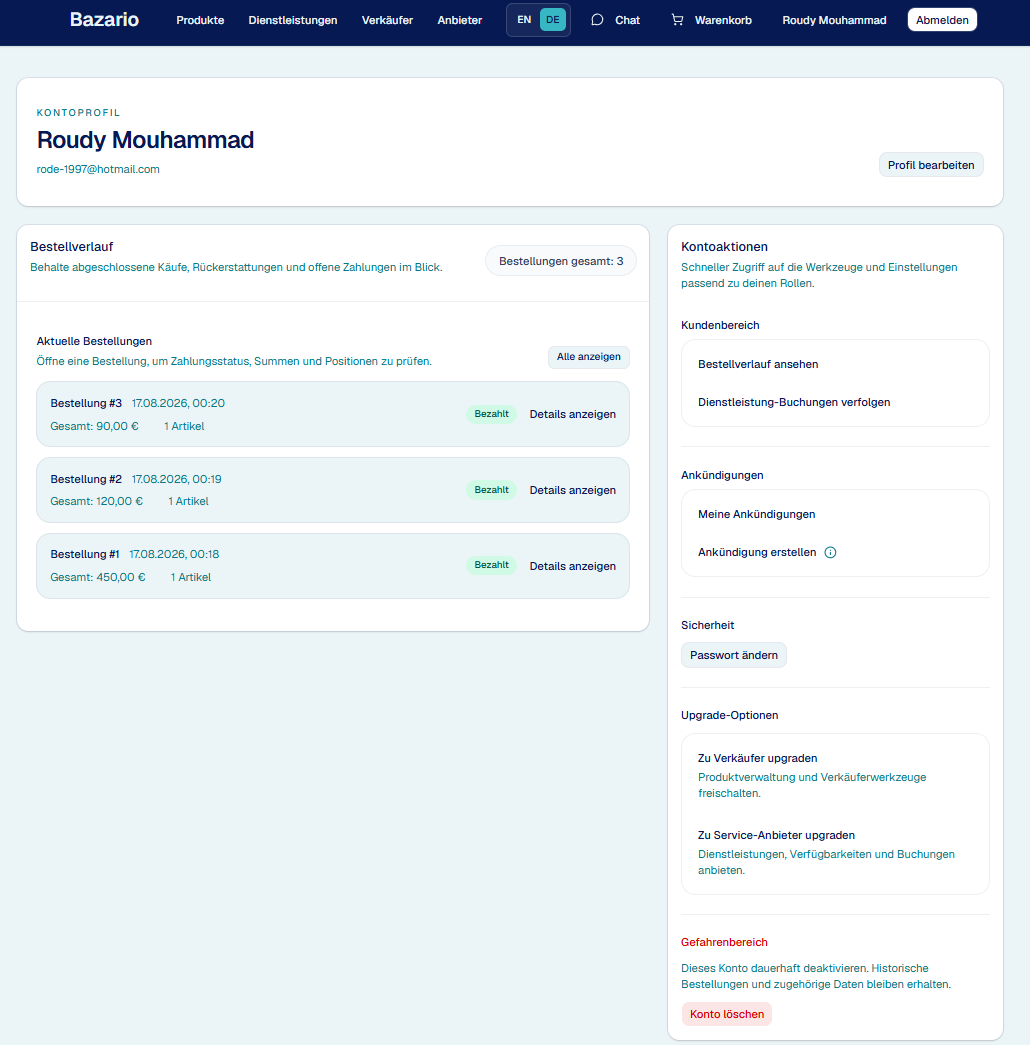
\includegraphics[width=0.85\textwidth]{Bilder/screenshot_kontoseite_kunde.png}
\caption{Kontoseite eines Nutzers ohne zusätzliche Rollen}
\label{fig:kontoseite_kunde}
\end{figure}
 
Für einen Nutzer ohne zusätzliche Rollen zeigt die rechte Spalte
allein den Kundenbereich, gefolgt von den rollenunabhängigen
Funktionen und den Anträgen auf ein Rollen-Upgrade. Die linke Spalte
enthält die eigene Bestellhistorie mit Datum, Betrag, Anzahl der
Positionen und Zahlungsstatus.
 
\begin{figure}[H]
\centering
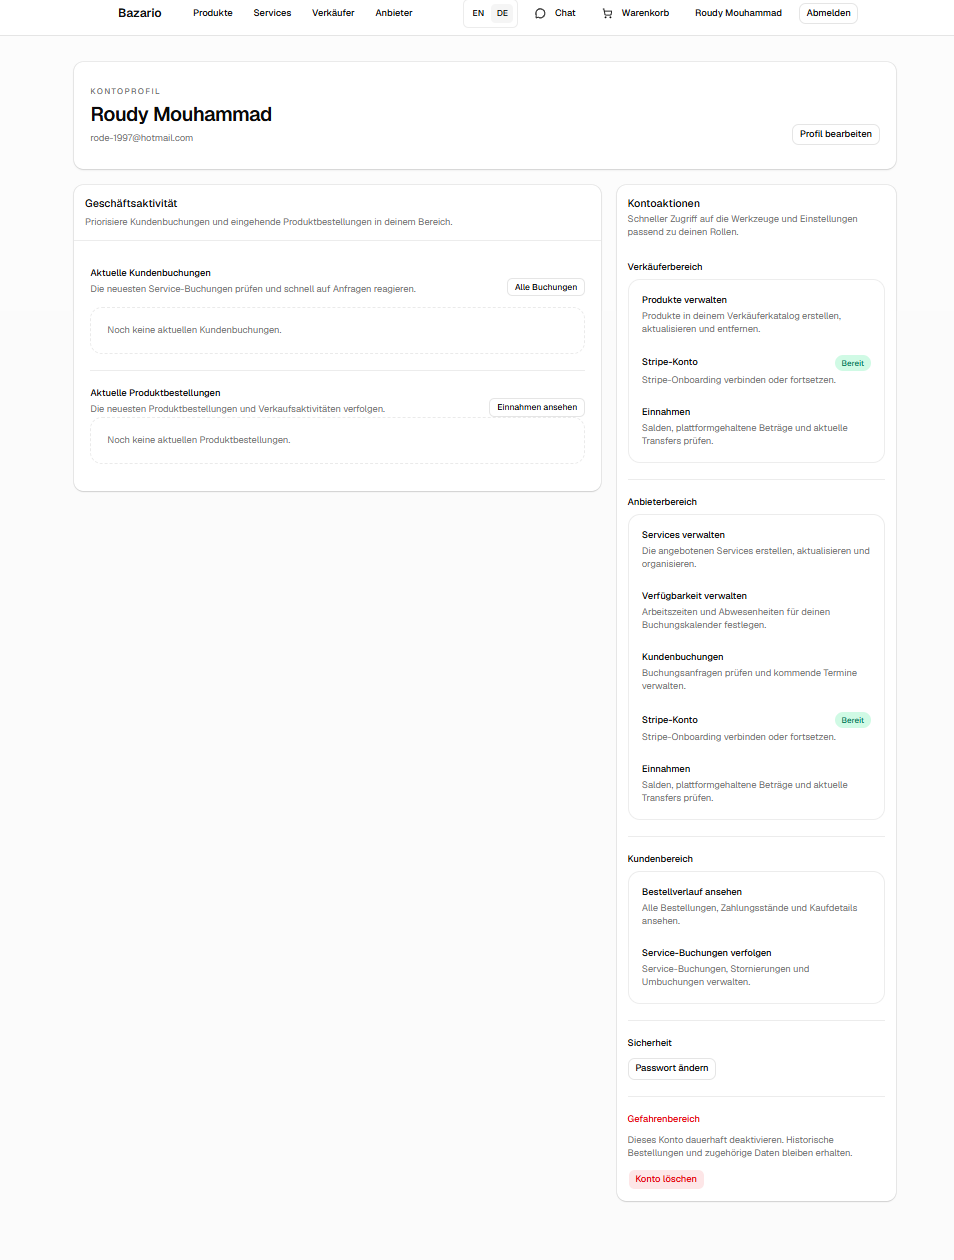
\includegraphics[width=0.85\textwidth]{Bilder/screenshot_kontoseite_anbieter.png}
\caption{Kontoseite eines Nutzers mit den Rollen 	extit{Seller} und
	extit{ServiceProvider}}
\label{fig:kontoseite_anbieter}
\end{figure}
 
Dieselbe Seite zeigt für einen Nutzer mit beiden anbietenden Rollen
drei Arbeitsbereiche untereinander: den Verkäuferbereich mit der
Produktverwaltung, den Anbieterbereich mit Dienstleistungen,
Verfügbarkeit und eingegangenen Buchungen sowie darunter den
Kundenbereich, den er als jeder andere Nutzer ebenfalls besitzt.
Anbindung an den Zahlungsdienst und Einnahmenübersicht erscheinen in
beiden anbietenden Bereichen, da sie für beide Rollen gelten.
 
Die Anträge auf ein Rollen-Upgrade entfallen hier vollständig. Sie
werden nur dann gerendert, wenn das Backend die jeweilige Rolle als
noch verfügbar meldet. Damit zeigt die Oberfläche keine Handlung an,
die für diesen Nutzer keine Wirkung mehr hätte.
 
Auch die linke Spalte wechselt mit der Rolle. Statt der eigenen
Bestellhistorie erscheint bei anbietenden Nutzern die
Geschäftsaktivität mit den eingegangenen Buchungen und
Produktbestellungen; die eigene Bestellhistorie wird darunter
zusätzlich eingeblendet, sofern eigene Bestellungen vorliegen.
Liegen für einen Bereich keine Einträge vor, erscheint an dessen
Stelle ein Hinweis statt einer leeren Fläche, wie er auch auf den
Katalogseiten verwendet wird (vgl.
Abschnitt~\ref{subsec:impl_produktlisting}).
 
Sämtliche Einträge der rechten Spalte werden über dieselbe
wiederverwendbare Komponente dargestellt, die Titel, Beschreibung,
Ziel und optional eine Zustandsmarkierung entgegennimmt. Aufbau und
Verhalten aller Einträge sind dadurch nicht durch Sorgfalt bei der
Umsetzung gleich, sondern durch Konstruktion. Die
Zustandsmarkierung wird bislang nur beim Zahlungsdienst verwendet
und zeigt dort an, ob das verbundene Konto eingerichtet ist. Ihre
Daten stammen aus einer eigenen Anfrage, die ausschließlich für
anbietende Nutzer ausgeführt wird.

\subsection{Dienstleistungsverwaltung: Zeitfenster und Abdeckungsbereich}
\label{subsec:impl_dienstleistungsverwaltung}
 
Dieser Abschnitt beschreibt sowohl die Verwaltung einzelner
Dienstleistungsangebote als auch die Verwaltung der Verfügbarkeit, die
als eigener Funktionsbereich \texttt{provider-availability/} umgesetzt
ist und derselben internen Struktur wie die übrigen Funktionsbereiche
folgt (vgl. Abschnitt~\ref{subsec:komponentenarchitektur}).
 
Die eigenen Dienstleistungen werden über \texttt{useMyServicesQuery}
abgerufen und seitenweise dargestellt; Seite und Ergebnisse pro Seite
sind, wie bereits beim Produktlisting beschrieben (vgl.
Abschnitt~\ref{subsec:impl_produktlisting}), Teil des Query Keys. Jede
Dienstleistung erscheint als Karte mit Kategorie, Preis, Dauer und
Veröffentlichungsstatus; gegenüber der öffentlichen Katalogansicht
ergänzt die Verwaltungskarte die Aktionen zum Ansehen, Bearbeiten und
Löschen.
 
\begin{figure}[H]
\centering
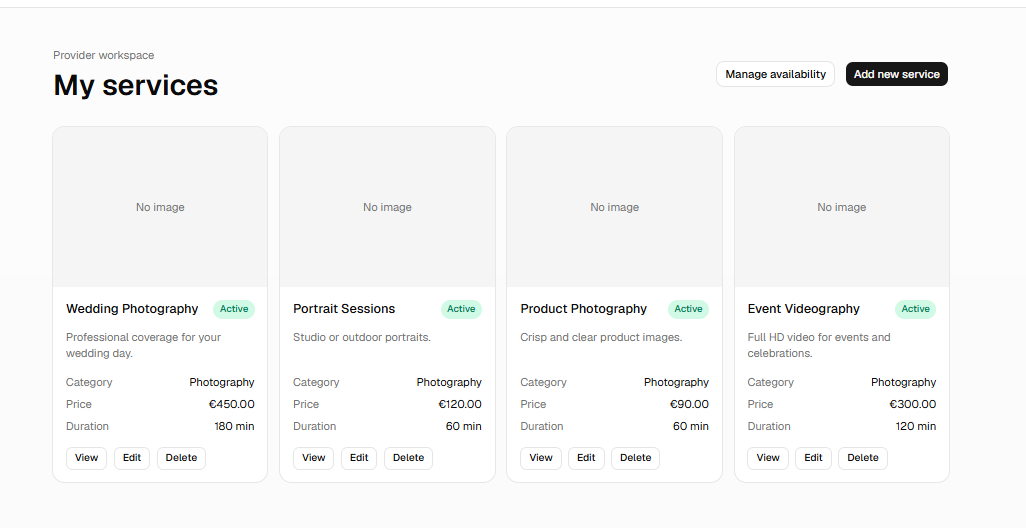
\includegraphics[width=\textwidth]{Bilder/screenshot_my_services.png}
\caption{Übersicht der eigenen Dienstleistungen mit den Aktionen zum Ansehen, Bearbeiten und Löschen}
\label{fig:my_services}
\end{figure}
 
Das Löschen einer Dienstleistung folgt demselben Muster wie die
Nebenwirkungen der Erfolgsseite (vgl.
Listing~\ref{lst:checkout-success}), betrifft jedoch vier
Zwischenspeicher zugleich: die eigene Übersicht, den öffentlichen
Dienstleistungskatalog, die zugehörige Detailseite und die
Startseite. Aus allen vieren muss der Eintrag zugleich verschwinden,
weshalb sie gezielt invalidiert werden, anstatt sich auf ein
automatisches Ablaufen zu verlassen (vgl.
Abschnitt~\ref{subsec:impl_tanstackquery}). Auf dem Bildschirm ist
davon nichts zu erkennen; sichtbar würde erst das Gegenteil, nämlich
eine Liste, in der ein bereits gelöschter Eintrag noch erscheint.
 
Beim Anlegen und Bearbeiten einer Dienstleistung werden neben Titel
und Beschreibung, die jeweils auf Englisch und Arabisch erfasst
werden, zugleich die Regeln für deren spätere Buchung festgelegt.
 
\begin{figure}[H]
\centering
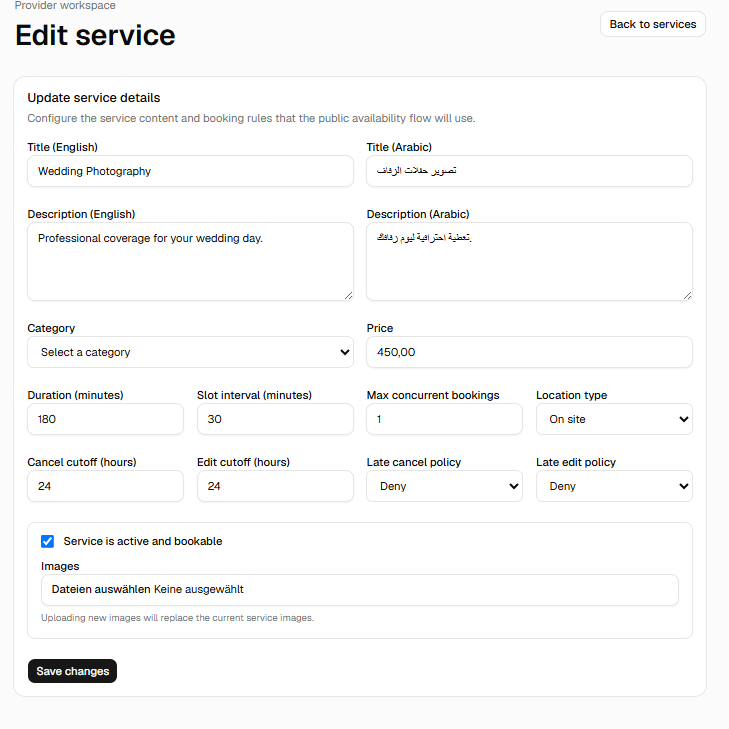
\includegraphics[width=\textwidth]{Bilder/screenshot_edit_service.png}
\caption{Formular zum Bearbeiten einer Dienstleistung mit
zweisprachigen Inhaltsfeldern und Buchungsregeln}
\label{fig:edit_service}
\end{figure}
 
Diese Regeln bestimmen, welche Termine die Buchungsansicht später
anbietet: Die Dauer legt die Länge eines Termins fest, das Zeitraster
den Abstand zwischen zwei möglichen Startzeitpunkten, und die maximale
Anzahl gleichzeitiger Buchungen bestimmt, wie viele Kunden denselben
Zeitraum belegen können. Hinzu kommen der Ort der Leistungserbringung
sowie getrennte Fristen für Stornierung und Änderung, jeweils mit der
Festlegung, wie nach Ablauf der Frist zu verfahren ist.
 
Die Verfügbarkeit wird davon getrennt verwaltet, da sie nicht für eine
einzelne Dienstleistung, sondern für alle Angebote eines Anbieters
gemeinsam gilt.
 
\begin{figure}[H]
\centering
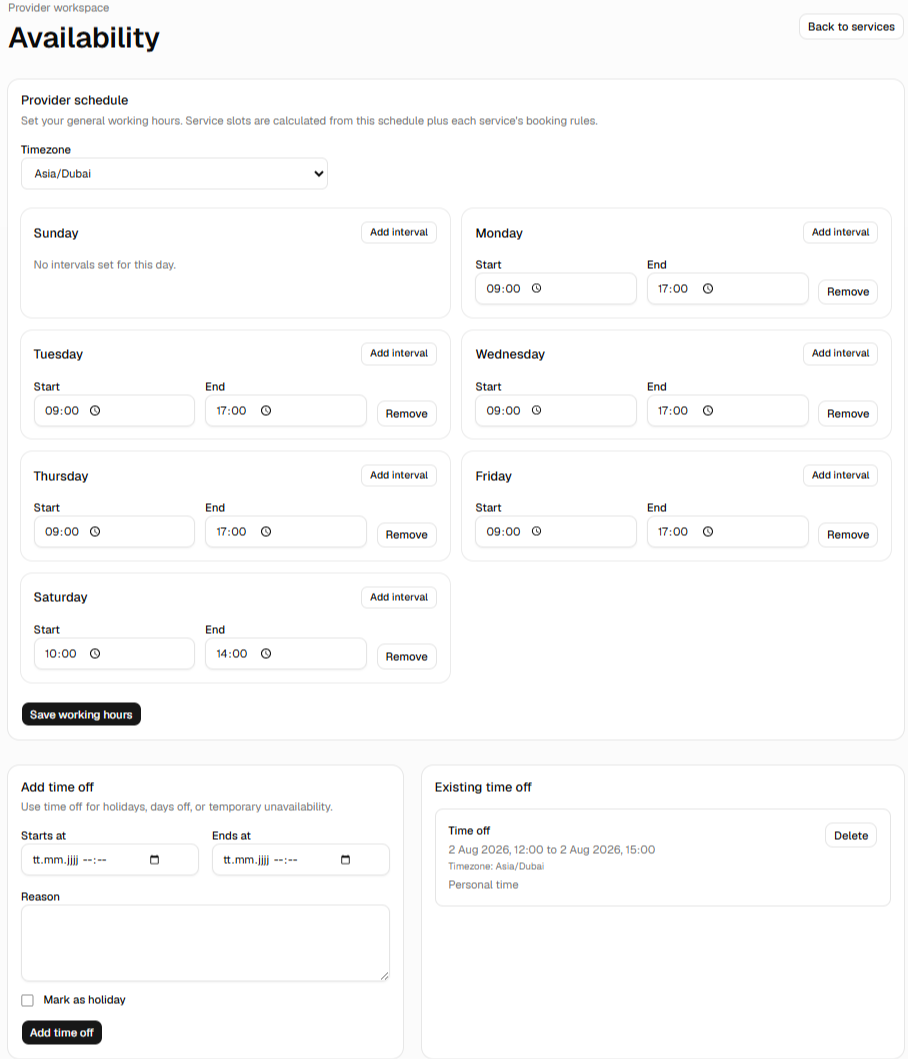
\includegraphics[width=0.7\textwidth]{Bilder/screenshot_availability.png}
\caption{Verfügbarkeitsverwaltung mit Wochenschema und einzelnen Abwesenheitszeiträumen}
\label{fig:availability}
\end{figure}
 
Die festen Arbeitszeiten werden je Wochentag über die
wiederverwendbare Komponente \texttt{WorkingHoursEditor} dargestellt,
die für jeden Wochentag beliebig viele Zeitintervalle mit Start- und
Endzeit entgegennimmt und es erlaubt, einzelne Intervalle hinzuzufügen
oder zu entfernen. Ein Wochentag ohne Intervall gilt als nicht
verfügbar.
 
Das Formular \texttt{TimeOffForm} für einzelne Abwesenheitszeiträume
ist als eigene Komponente ausgelagert, da es an mehreren Stellen
innerhalb des Funktionsbereichs wiederverwendet wird. Seine Eingaben
werden über ein Zod-Schema validiert (vgl.
Abschnitt~\ref{subsec:formulare-validierung}), das bewusst mit den
Validierungsregeln des Backends übereinstimmt, sodass ein Nutzer, der
die Formularvalidierung durch direkte Manipulation der
Benutzeroberfläche umgeht, spätestens bei der serverseitigen Prüfung
denselben Regeln unterliegt.
 
Der Abruf der Verfügbarkeitsdaten erfolgt über
\texttt{useProviderAvailabilityQuery}, das Hinzufügen eines
Abwesenheitszeitraums über eine Mutation, die den zugehörigen
Cache-Eintrag im Erfolgsfall invalidiert, sodass die Liste automatisch
aktualisiert wird. Die eingetragenen Zeiträume werden nach ihrem
Beginn sortiert angezeigt und anhand der beim Anbieter hinterlegten
Zeitzone formatiert, nicht anhand der Zeitzone des aufrufenden
Endgeräts, damit Kunden die Verfügbarkeit unabhängig vom eigenen
Standort korrekt einschätzen können.
\subsection{Produktverwaltung}
\label{subsec:impl_produktverwaltung}

Die Produktverwaltung folgt strukturell demselben Muster wie die
in Abschnitt~\ref{subsec:impl_dienstleistungsverwaltung}
beschriebene Dienstleistungsverwaltung, ist jedoch einfacher, da
Produkte im Gegensatz zu Dienstleistungen keine Buchungsregeln
benötigen.

% TODO (Roudy): Hier kommt der Screenshot von "My products"
% hin (Kartenuebersicht der eigenen Produkte).

Die eigenen Produkte werden über \texttt{useMyProductsQuery}
abgerufen und nach demselben Kartenprinzip dargestellt, das auch
auf der öffentlichen Katalogseite zum Einsatz kommt (vgl.
Abschnitt~\ref{subsec:impl_produktlisting}); die
Verwaltungskarte ergänzt dabei Aktionen zum Bearbeiten
und Löschen. Das Löschen eines Produkts verfährt ebenso, betrifft aber nur drei
Zwischenspeicher, da eine eigene Detailseite im Zwischenspeicher
nicht gesondert geführt wird: die eigene Produktliste, den
öffentlichen Katalog und die Produkte des Verkäuferprofils.

% TODO (Roudy): Hier kommt der Screenshot vom "Edit product"-
% Formular hin.

Die erfassten Felder entsprechen dabei denen der
Dienstleistungsverwaltung, abzüglich der dort beschriebenen
Buchungsregeln (vgl.
Abschnitt~\ref{subsec:verkaeufer_dashboard_konzept}).


\subsection{Eingegangene Buchungen}
\label{subsec:impl_provider_bookings}
Die Ansicht der eingegangenen Buchungen setzt die in
Abschnitt~\ref{subsec:verkaeufer_dashboard_konzept} beschriebene
Zustandsfolge um. Jede Buchung erscheint als Eintrag mit Kunde,
Beginn, Ende und Zeitzone sowie einer Zustandsmarkierung.
 
\begin{figure}[H]
\centering
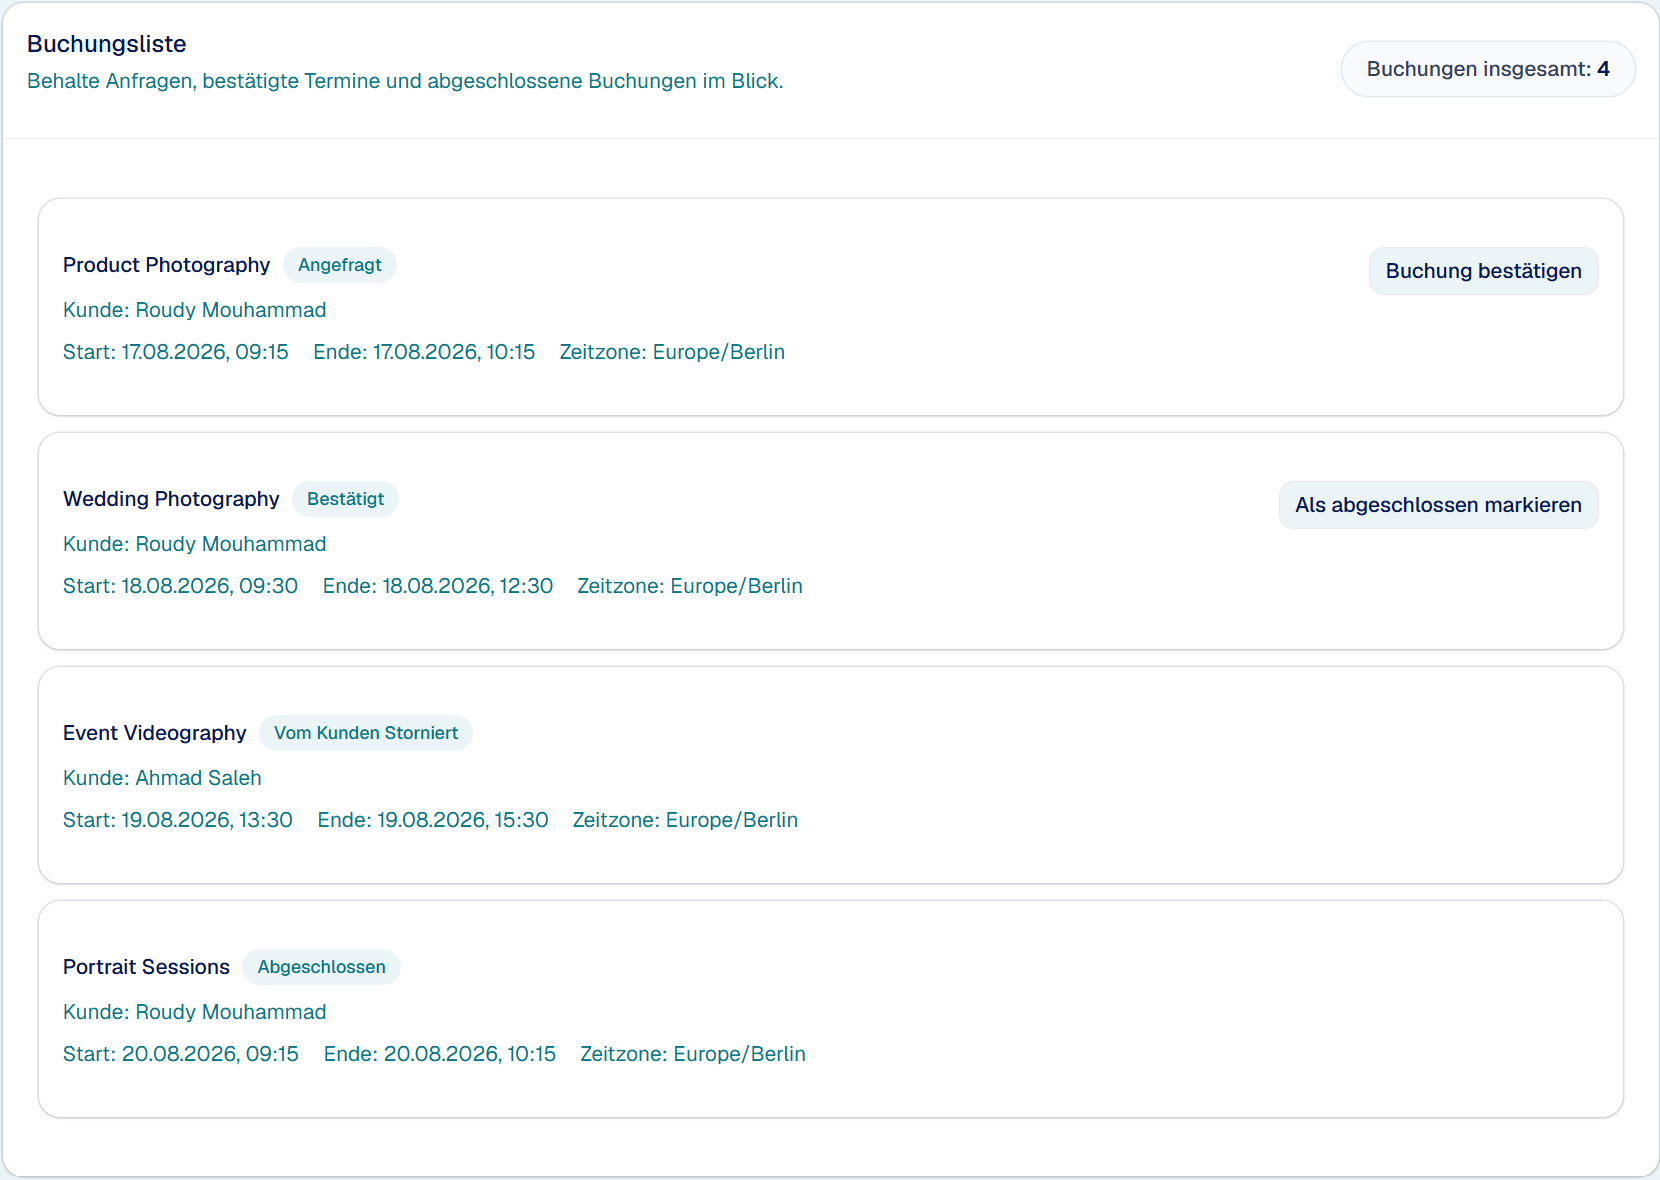
\includegraphics[width=\textwidth]{Bilder/screenshot_provider_bookings.png}
\caption{Eingegangene Buchungen mit der jeweils zustandsabhängigen
Aktion}
\label{fig:provider_bookings}
\end{figure}
 
Rechts neben jedem Eintrag steht genau eine Schaltfläche, und welche
das ist, ergibt sich aus dem Zustand: Bei einer angefragten Buchung
lautet sie \textit{Buchung bestätigen}, bei einer bereits bestätigten
\textit{Als abgeschlossen markieren}. Eine abgeschlossene Buchung
trägt keine Schaltfläche mehr. Die Oberfläche zeigt damit nicht alle
denkbaren Aktionen mit wechselnder Verfügbarkeit, sondern jeweils nur
die eine, die im gegenwärtigen Zustand möglich ist.
 
Beide Übergänge sind als Mutationen umgesetzt, die den
zwischengespeicherten Bestand der Buchungsliste im Erfolgsfall
invalidieren (vgl. Abschnitt~\ref{subsec:impl_tanstackquery}), sodass
der neue Zustand unmittelbar erscheint, ohne dass die Seite neu
geladen werden muss.


\subsection{Bestellhistorie und Bestelldetail}
\label{subsec:impl_bestellungen}

Die Bestellübersicht führt sämtliche Aufträge des Nutzers mit Datum,
Gesamtbetrag, Anzahl der Positionen und Zahlungsstatus. Der Aufruf
eines Eintrags führt auf die Detailseite, die den Auftrag in zwei
Bereiche gliedert: eine Zusammenfassung mit den Kopfdaten und die
Liste der enthaltenen Positionen.
 
Da ein Auftrag bereits vor der Zahlung entsteht (vgl.
Abschnitt~\ref{subsec:warenkorb_konzept}), unterscheidet die
Detailseite zwei Fälle. Bei einem unbezahlten Auftrag tritt an die
Stelle der Positionsliste ein eigener Bereich, der den Zustand
benennt und zwei Wege anbietet.
 
\begin{figure}[H]
\centering
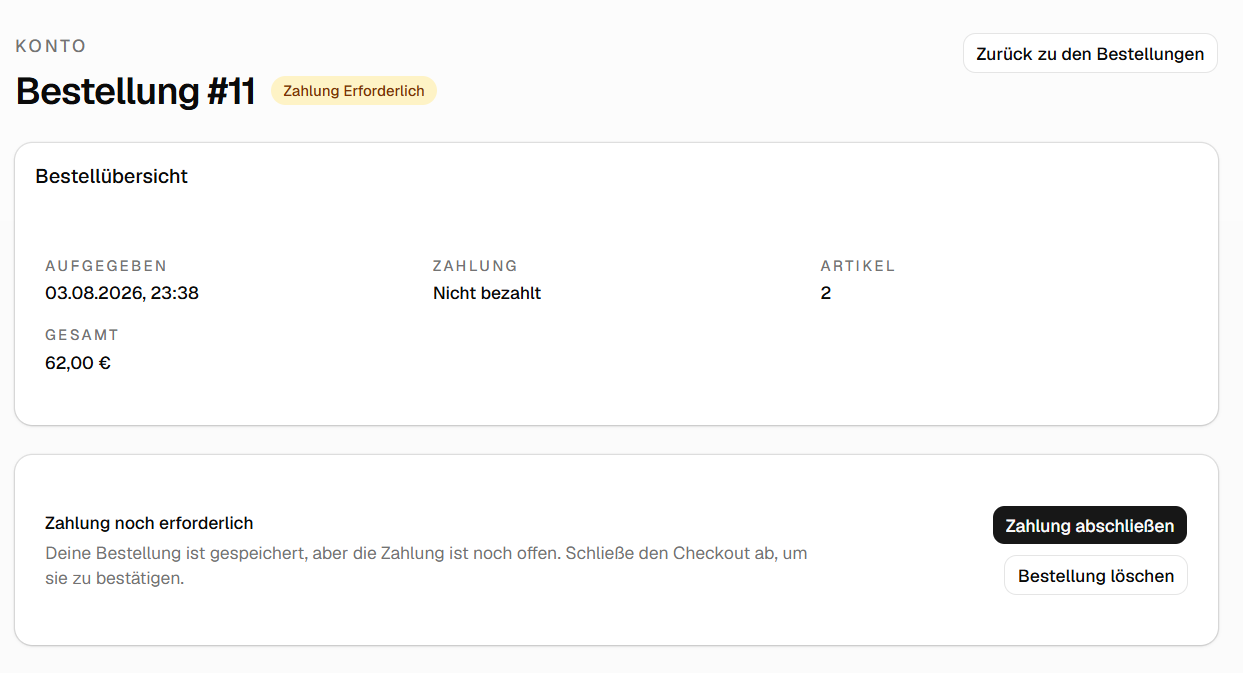
\includegraphics[width=\textwidth]{Bilder/screenshot_bestellung_unbezahlt.png}
\caption{Detailansicht eines Auftrags, dessen Zahlung nicht
abgeschlossen wurde}
\label{fig:bestellung_unbezahlt}
\end{figure}
 
Verlässt ein Nutzer die Zahlungsseite, ohne den Vorgang
abzuschließen, bleibt der Auftrag in diesem Zustand bestehen. Er
lässt sich entweder nachträglich bezahlen oder verwerfen. Ohne diese
beiden Möglichkeiten entstünde bei jedem abgebrochenen
Zahlungsvorgang ein Eintrag, den der Nutzer weder abschließen noch
entfernen könnte. Der Fall betrifft Produkte und
Dienstleistungsbuchungen gleichermaßen.
 
Bei einem bezahlten Auftrag erscheint dagegen die vollständige
Positionsliste. Jede Position trägt ihren eigenen Zustand, da
Produkte und Dienstleistungen unabhängig voneinander bearbeitet
werden.
 
\begin{figure}[H]
\centering
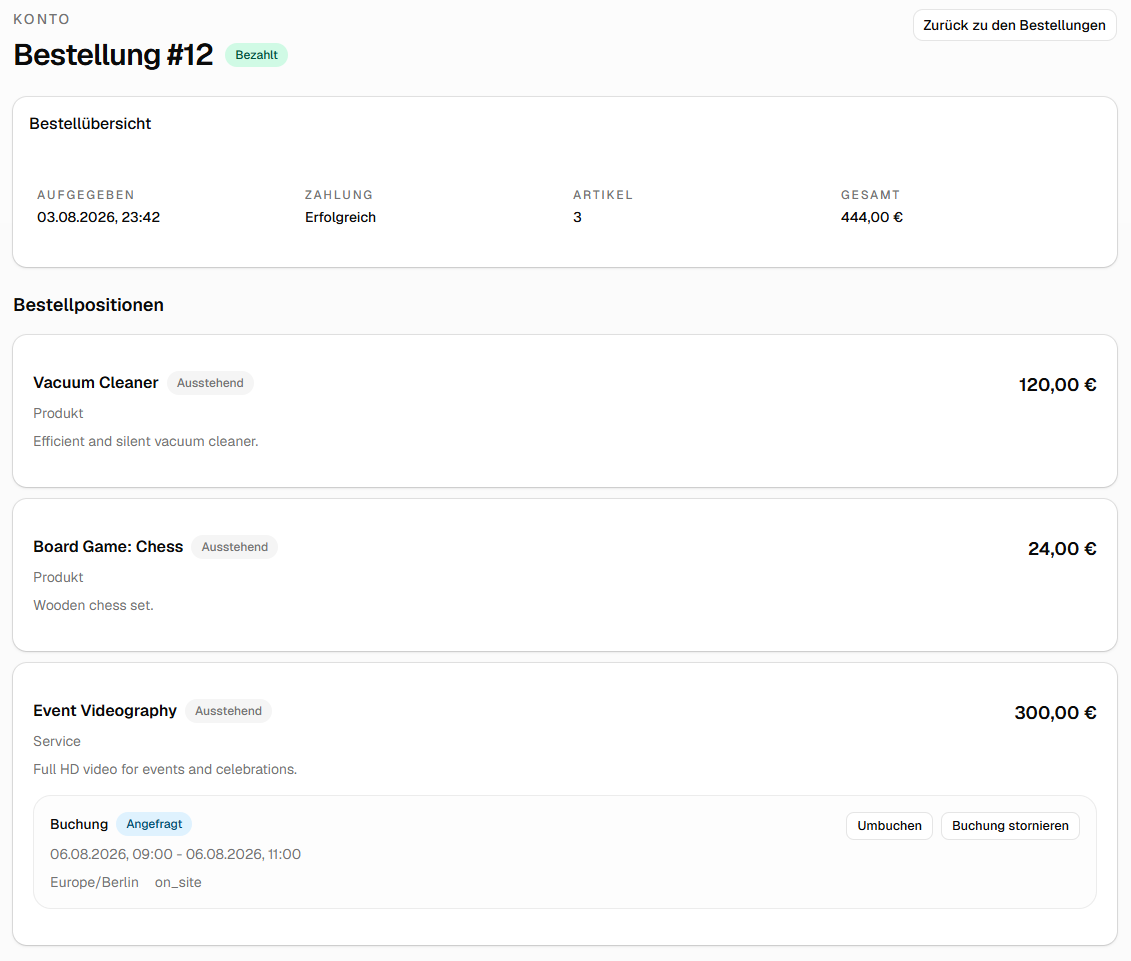
\includegraphics[width=0.85\textwidth]{Bilder/screenshot_bestelldetail.png}
\caption{Detailansicht eines bezahlten Auftrags mit Produkt- und
Dienstleistungspositionen}
\label{fig:bestelldetail}
\end{figure}
 
Eine Dienstleistungsposition führt dabei die zugehörige Buchung mit:
Termin, Zeitzone und Ort der Leistungserbringung erscheinen innerhalb
der Position, zusammen mit den Schaltflächen zum Umbuchen und
Stornieren. Dieselben Aktionen sind auch über die Buchungsübersicht
erreichbar (vgl. Abschnitt~\ref{subsec:impl_buchungen}). Die
doppelte Erreichbarkeit ist beabsichtigt: Ein Nutzer, der von einer
Bestellung ausgeht, soll die zugehörige Buchung nicht in einer
anderen Ansicht suchen müssen.

\subsection{Buchungsübersicht, Stornierung und Umbuchung}
\label{subsec:impl_buchungen}

Die Buchungsübersicht führt die gebuchten Termine des Nutzers mit
Dienstleistung, Anbieter, Zeitraum, Zeitzone, Ort und Zustand. Unter
jedem Eintrag stehen zwei Blöcke, einer für die Stornierung und einer
für die Umbuchung, in denen die beim Anlegen der Dienstleistung
festgelegten Fristen wiedergegeben werden (vgl.
Abschnitt~\ref{subsec:impl_dienstleistungsverwaltung}). Solange eine
Frist läuft, nennt der zugehörige Block den Zeitpunkt ihres Endes,
und die Schaltfläche ist auslösbar.
 
\begin{figure}[H]
\centering
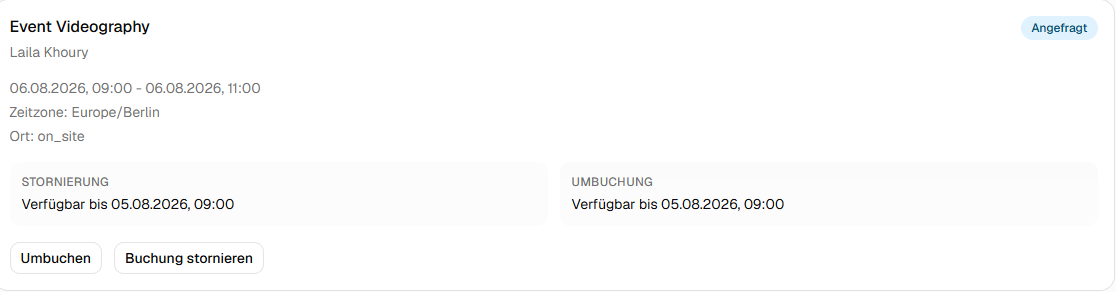
\includegraphics[width=\textwidth]{Bilder/screenshot_buchung_offen.png}
\caption{Buchung innerhalb der Fristen: beide Aktionen verfügbar,
jeweils mit Angabe des Fristendes}
\label{fig:buchung_offen}
\end{figure}
 
Nach Ablauf einer Frist wird die zugehörige Schaltfläche deaktiviert,
und an die Stelle des Fristendes tritt der Hinweis, dass der Zeitraum
verstrichen ist. Beide Schaltflächen bleiben dabei sichtbar --
dieselbe Entscheidung wie bei der Terminauswahl, in der ein nicht
verfügbarer Tag benannt statt ausgeblendet wird (vgl.
Abschnitt~\ref{subsec:impl_terminauswahl}).
 
\begin{figure}[H]
\centering
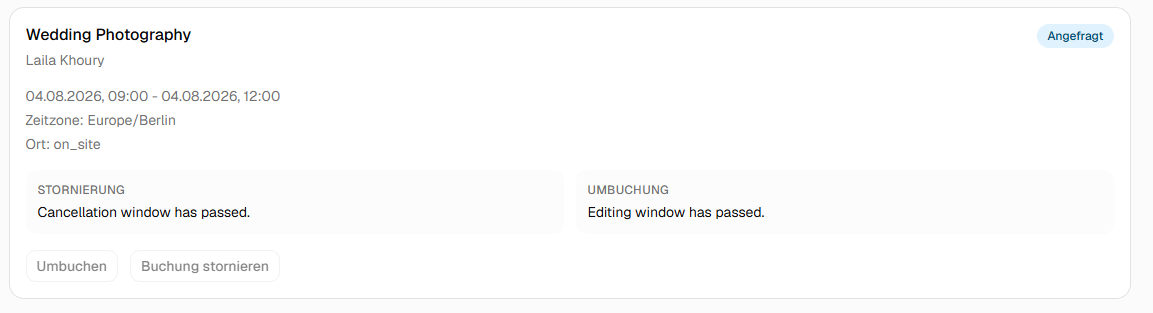
\includegraphics[width=\textwidth]{Bilder/screenshot_buchung_frist_abgelaufen.png}
\caption{Buchung nach Ablauf beider Fristen: die Schaltflächen sind
deaktiviert, der Grund steht darüber}
\label{fig:buchung_frist_abgelaufen}
\end{figure}
 
Die Umbuchung führt auf eine eigene Seite, die dieselbe
Terminauswahl verwendet wie die Erstbuchung. Die Komponente ist damit
an zwei Stellen der Anwendung eingesetzt, ohne dass die Ermittlung
verfügbarer Zeitfenster ein zweites Mal umgesetzt werden musste.
Neben der Auswahl zeigt die Seite den bisherigen Termin, sodass der
Wechsel nachvollziehbar bleibt.
 
Eine Stornierung löst dagegen keine erneute Auswahl aus, sondern eine
Rückerstattung über das Backend, deren Stand anschließend an der
Buchung selbst geführt wird.

% ----------------------------------------------------------------

\section{Werbung und Ankündigungen}
\label{sec:impl_werbung}

% TODO: Implementierung der Ankündigungen und Werbemodule je Rolle,
% Genehmigungsprozess.

% ----------------------------------------------------------------
\section{Messaging}
\label{sec:impl_messaging}
Die Umsetzung des in Abschnitt~\ref{subsec:messaging_konzept}
beschriebenen Nachrichtenbereichs besteht aus zwei Teilen, die
unabhängig voneinander arbeiten: dem gewöhnlichen, anfragebasierten
Zugriff auf Unterhaltungen und Nachrichten und der Anbindung an den
Echtzeitdienst. Der erste Teil folgt dem in
Abschnitt~\ref{subsec:impl_featureapi} beschriebenen Aufbau und
verwendet dieselbe \acs{HTTP}-Instanz wie alle übrigen
Funktionsbereiche; er liefert die Liste der Unterhaltungen, den
Verlauf einer Unterhaltung und den Zählerstand ungelesener
Nachrichten und nimmt gesendete Nachrichten entgegen. Der zweite
Teil ist Gegenstand dieses Abschnitts.
 
 
\subsection{Anbindung des Echtzeitdienstes}
\label{subsec:impl_pusher_client}
 
Die Verbindung wird in einem eigenen Modul gekapselt, das als
einzige Stelle der Anwendung die Bibliothek des Dienstanbieters
kennt. Es hält die Verbindung in einer Modulvariablen und gibt eine
bereits bestehende Verbindung zurück, statt eine zweite aufzubauen.
Diese Festlegung ist notwendig, weil mehrere Stellen der Anwendung
unabhängig voneinander Kanäle abonnieren: die Chatseite für jede
Unterhaltung und die Kopfzeile für den Zählerstand. Ohne die
Bündelung entstünde je Aufruf eine eigene Verbindung.
 
\begin{lstlisting}[language=TypeScript,caption={Aufbau der Verbindung
zum Echtzeitdienst},label={lst:pusher-client}]
let client: Pusher | null = null
 
export function getPusherClient() {
  const token = getAuthToken()
  const config = getPusherConfig()
 
  if (!token || !config) {
    return null
  }
 
  if (client) {
    return client
  }
 
  client = new Pusher(config.key, {
    cluster: config.cluster,
    authEndpoint: getBroadcastAuthEndpoint(),
    auth: {
      headers: { Authorization: `Bearer ${token}` },
    },
  })
 
  return client
}
\end{lstlisting}
 
Drei Angaben bestimmen die Verbindung. Der Schlüssel identifiziert
das Projekt beim Dienstanbieter. Der \emph{Cluster} benennt die
Region, in der die Kanäle betrieben werden, und ist damit für die
Laufzeit einer Nachricht maßgeblich. Der dritte Wert ist die
Adresse, an die der Dienst seine Freigabeanfragen richtet: Meldet
sich der Client für einen privaten Kanal an, fragt die Bibliothek
zunächst beim Backend nach, ob er dazu berechtigt ist. Da diese
Anfrage nicht über die zentrale \acs{HTTP}-Instanz aus
Abschnitt~\ref{subsec:impl_httpclient} läuft, sondern von der
Bibliothek selbst gestellt wird, muss der Authentifizierungstoken
hier ein zweites Mal ausdrücklich mitgegeben werden.
 
Ohne angemeldeten Nutzer liefert die Funktion keinen Client. Der
Nachrichtenbereich ist damit auch technisch an die Anmeldung
gebunden und nicht allein über den Routenschutz aus
Abschnitt~\ref{subsec:impl_token_session}.
 
 
\subsection{Nachrichtenoberfläche}
\label{subsec:impl_chat_ui}
 
Die Chatseite ist zweispaltig aufgebaut. Links steht die Liste der
Unterhaltungen mit Name des Gegenübers, Zeitpunkt und Anfang der
letzten Nachricht, rechts der Verlauf der ausgewählten Unterhaltung.
Die gewählte Unterhaltung steht als Bestandteil der Adresse
(\texttt{/chat/:conversationId}), sodass eine einzelne Unterhaltung
verlinkbar bleibt -- dieselbe Entscheidung wie bei den Katalogseiten,
auf denen Seite und Kategorie ebenfalls in der Adresse stehen (vgl.
Abschnitt~\ref{subsec:impl_produktlisting}).
Ist keine Unterhaltung angegeben, wird auf die zuletzt aktive
umgeleitet.
 
\begin{figure}[H]
\centering
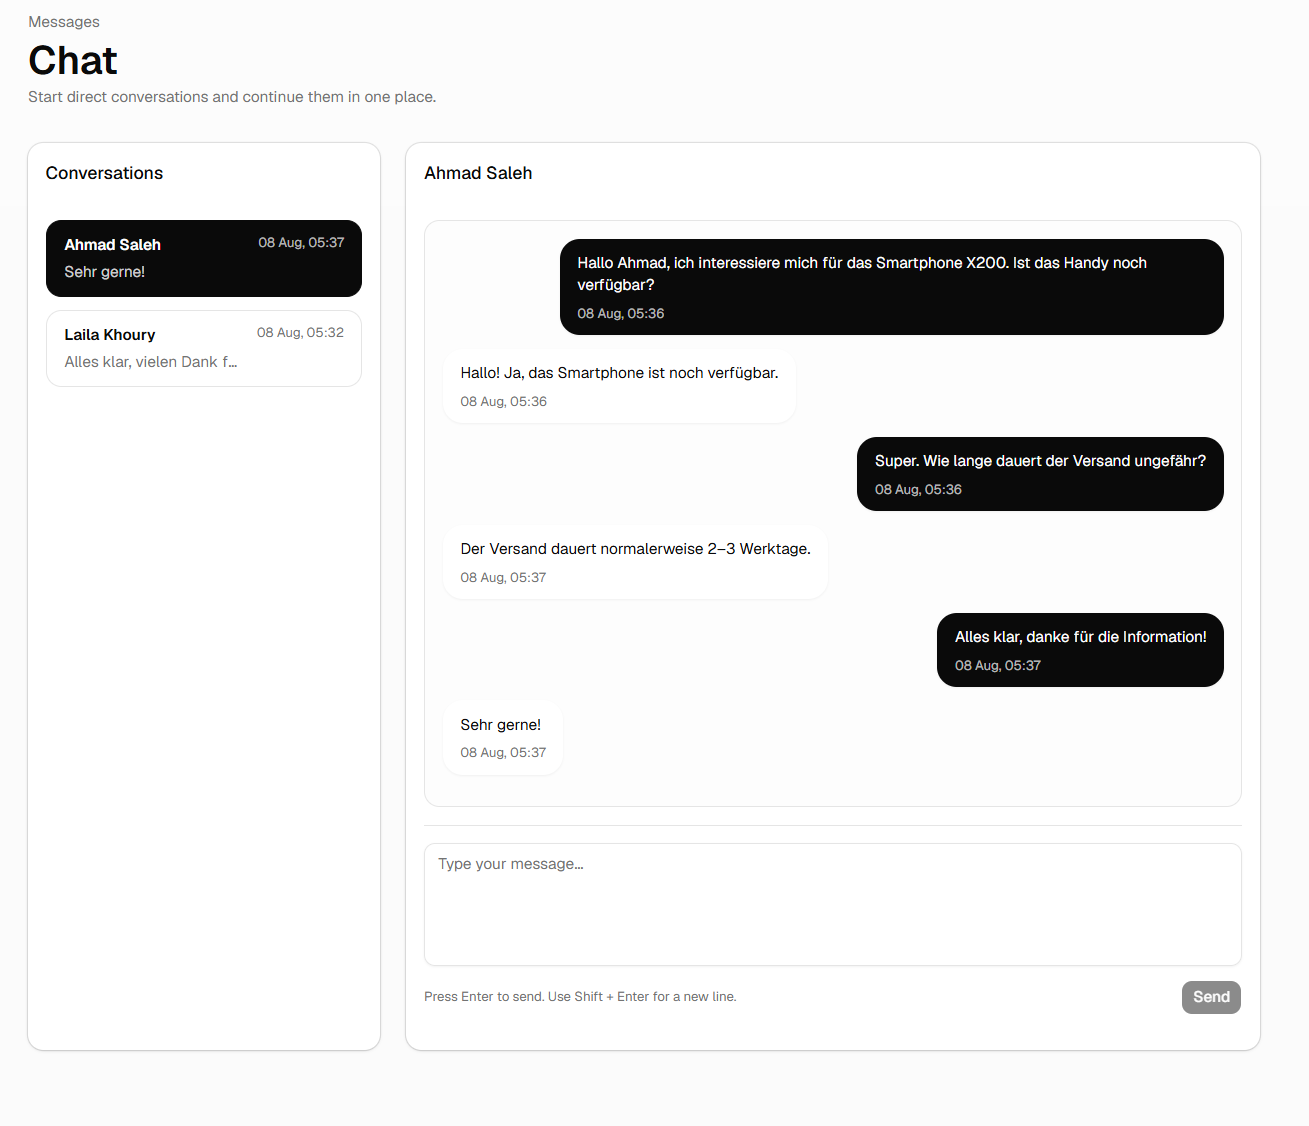
\includegraphics[width=\textwidth]{Bilder/screenshot_chat.png}
\caption{Nachrichtenbereich mit Liste der Unterhaltungen und
Verlauf}
\label{fig:chat_seite}
\end{figure}
 
Eigene und empfangene Nachrichten unterscheiden sich in Ausrichtung
und Farbe. Die Zuordnung erfolgt nicht über die Reihenfolge, sondern
über den Vergleich der Absenderkennung mit der Kennung des
angemeldeten Nutzers -- eine Nachricht, die über den Kanal
eintrifft, trägt dieselbe Struktur wie eine aus der Datenbank
geladene und wird deshalb gleich behandelt.
 
Die Unterhaltungen werden nach dem Zeitpunkt der letzten Nachricht
sortiert, sodass die zuletzt genutzte oben steht. Da diese
Sortierung sowohl beim Laden als auch beim Eintreffen einer
Nachricht über den Kanal angewendet werden muss, ist sie als eigene
Funktion ausgelagert.
 
 
\subsection{Abonnement der Kanäle und Aktualisierung des
Zwischenspeichers}
\label{subsec:impl_chat_realtime}
 
Sobald die Liste der Unterhaltungen vorliegt, meldet sich die Seite
für jede darin enthaltene Unterhaltung beim zugehörigen Kanal an.
Die Kanalnamen ergeben sich unmittelbar aus der Kennung der
Unterhaltung, sodass keine gesonderte Zuordnung geführt werden muss.
Auf jedem Kanal werden drei Ereignisse ausgewertet: das Eintreffen
einer Nachricht sowie die Bestätigung ihrer Zustellung und ihres
Lesens.
 
Entscheidend ist, was beim Eintreffen eines Ereignisses geschieht.
Die Anwendung stellt keine neue Anfrage an das Backend, sondern
schreibt die empfangene Nachricht unmittelbar in den
Zwischenspeicher von TanStack Query (vgl.
Abschnitt~\ref{subsec:impl_tanstackquery}). Eine erneute Anfrage wäre
überflüssig, da die Nachricht bereits vollständig vorliegt; sie
würde die Ersparnis, die die dauerhafte Verbindung gerade bewirkt,
wieder aufheben.
 
\begin{lstlisting}[language=TypeScript,caption={Eintragen einer über
den Kanal empfangenen Nachricht in den Zwischenspeicher},
label={lst:chat-cache}]
queryClient.setQueryData<ChatMessagesResponse | undefined>(
  ['chat', 'messages', conversationId],
  (currentData) => {
    if (!currentData?.result) {
      return currentData
    }
 
    if (currentData.result.data.some((m) => m.id === normalizedMessage.id)) {
      return currentData
    }
 
    return {
      ...currentData,
      result: {
        ...currentData.result,
        data: [...currentData.result.data, normalizedMessage],
        total: currentData.result.total + 1,
      },
    }
  },
)
\end{lstlisting}
 
Die Prüfung auf eine bereits vorhandene Kennung ist erforderlich,
weil der Absender seine eigene Nachricht auf zwei Wegen erhält:
einmal als Antwort auf die absendende Anfrage und einmal über den
Kanal, auf dem sie veröffentlicht wird. Ohne diese Prüfung erschiene
sie doppelt.
 
Parallel dazu wird die Liste der Unterhaltungen fortgeschrieben:
Vorschautext und Zeitpunkt der betroffenen Unterhaltung werden
ersetzt, die Liste neu sortiert und der Zähler ungelesener
Nachrichten erhöht -- letzteres nur dann, wenn die Nachricht nicht
vom Nutzer selbst stammt und die betroffene Unterhaltung nicht gerade
geöffnet ist.
 
Die Anmeldung an den Kanälen erfolgt in einem Effekt, dessen
Aufräumfunktion die Ereignisbindungen löst und die Kanäle wieder
abmeldet. Unterbleibt dies, laufen nach einem Wechsel der Seite
weiterhin Ereignisse in Funktionen, die auf einen nicht mehr
dargestellten Zustand zugreifen; zugleich blieben die Kanäle
abonniert und die Zahl der Abonnements stiege mit jedem Aufruf der
Seite. Aus demselben Grund wird die Liste der Unterhaltungen mit
\texttt{useMemo} stabil gehalten: Entstünde bei jedem Rendern ein
neues Feld, liefe der Effekt jedes Mal erneut und meldete sämtliche
Kanäle ab und wieder an.
 
Der Zähler ungelesener Nachrichten in der Kopfzeile ist in einem
eigenen Hook gekapselt, der den auf den Nutzer bezogenen Kanal
abonniert und den empfangenen Gesamtstand in denselben
Zwischenspeicher schreibt, aus dem die Anzeige liest. Er ist
unabhängig von der Chatseite und damit in der gesamten Anwendung
wirksam.
 
Wird eine Unterhaltung geöffnet, prüft die Seite, ob sie ungelesene
Nachrichten des Gegenübers enthält, meldet sie gegebenenfalls als
gelesen und setzt den Zähler der betroffenen Unterhaltung
anschließend lokal auf null, ohne die Liste erneut abzurufen.

    \chapter{Testen und Bewertung}
\label{chap:testen}

Die Umsetzung wurde durch automatisierte Tests, eine heuristische
Evaluation der Oberfläche und die Prüfung ausgewählter
Erfolgskriterien der \acs{WCAG}~2.1 bewertet. Von den vier geprüften Kriterien sind drei erfüllt; der einzige
Verstoß betrifft den Kontrast des Fokusrings.

\section{Automatisierte Tests}
\label{sec:automatisierte_tests}

Die Anwendung enthält 36 Testdateien, die mit \textit{Vitest} und der
\textit{Testing Library} ausgeführt werden und fehlerfrei durchlaufen
(vgl. Abschnitt~\ref{sec:technologieauswahl}). Geprüft werden sowohl
reine Funktionen, etwa die Warenkorbsumme und Datumsaufbereitung, als
auch Komponenten wie Anmelde- und Registrierungsformulare. Ein
besonders relevanter Befund betraf eine fehlerhafte
Datumsformatierung, für die ein Test ergänzt wurde.

End-to-End-Tests mit \textit{Playwright} ergänzen die Modultests durch
die Prüfung vollständiger Nutzerabläufe. Ihre Einrichtung ist noch
nicht abgeschlossen.

\section{Heuristische Evaluation}
\label{sec:heuristische_evaluation}
Die Wahl der heuristischen Evaluation folgt aus den Rahmenbedingungen
der Arbeit. Ein Nutzertest hätte Teilnehmer und eine eigene Auswertung
erfordert und war zeitlich nicht leistbar; die im Unternehmen
vorgesehene Oberflächenprüfung findet erst an einer Vorabfassung und
durch eine andere Person statt. Erforderlich war deshalb ein
Verfahren, das sich von einer Person am eigenen Entwicklungsstand
anwenden lässt und mit den neun Heuristiken zugleich ein Raster über
die gesamte Oberfläche legt (vgl. Tabelle~\ref{tab:heuristiken}).
Die Evaluation folgt dem Verfahren von Nielsen und Molich
\cite{nielsen_molich_heuristic, nielsen_explanatory_power}. Es wurden
nur Befunde mit Ursache im Frontend berücksichtigt. 15 Befunde wurden
nach Nielsens Schweregradskala von null bis vier bewertet
\cite{nielsen_explanatory_power}; sechs weitere Beobachtungen wurden
nach Prüfung des Quellcodes ausgeschlossen.

\begin{table}[H]
\centering
\caption{Befunde der Evaluation}
\label{tab:befunde}
\small
\begin{tabular}{|l|p{4.6cm}|p{3.1cm}|c|l|}
\hline
\textbf{Nr} & \textbf{Befund} & \textbf{Heuristik} & \textbf{Grad} & \textbf{Status} \\
\hline
B1 & Anbieterbereich bei laufendem Antrag & Systemstatus & 3 & behoben \\
\hline
B2 & Hinterlegte Meldung wird nicht erreicht & Fehlerbehebung & 2 & behoben \\
\hline
B3 & Meldung benennt andere Regel & Fehlerbehebung & 2 & behoben \\
\hline
B4 & Storno nach Fristablauf & Fehlervermeidung & 3 & behoben \\
\hline
B5 & Überlappende Buchungszeiten & Fehlervermeidung & 2 & behoben \\
\hline
B6 & Rollenbereiche ohne Übersetzung & Reale Welt & 3 & behoben \\
\hline
B7 & Telefonfeld nicht als optional erkennbar & Wiedererkennung & 1 & geklärt \\
\hline
B8 & Erfolgsseite bietet beide Übersichten & Minimalismus & 2 & behoben \\
\hline
B9 & Interner Bezeichner in der Oberfläche & Reale Welt & 2 & behoben \\
\hline
B10 & Sprachwahl nicht ans Backend übertragen & Reale Welt & 3 & behoben \\
\hline
B11 & Positionsstatus widerspricht der Buchung & Systemstatus & 2 & behoben \\
\hline
B12 & Zwei gleichrangige Rückwege & Konsistenz & 2 & behoben \\
\hline
B13 & Englische Abkürzung in der Oberfläche & Reale Welt & 1 & behoben \\
\hline
B14 & Umbuchen auf Deutsch unbenutzbar & Fehlervermeidung & \textbf{4} & behoben \\
\hline
B15 & Eigenes Angebot buch- und kaufbar & Fehlervermeidung & 3 & behoben \\
\hline
\end{tabular}
\end{table}

Zusätzlich wurden drei technische Beobachtungen ohne
Usability-Schweregrad festgestellt: die nicht getrennte
Echtzeitverbindung beim Abmelden, wachsende Kanalabonnements und feste
Rückfallwerte im Quelltext. Die ersten beiden werden in
Kapitel~\ref{chap:fazit} aufgegriffen.

Auffällig ist die Häufung sprachbezogener Befunde. Vier der 15
Befunde betreffen die Übereinstimmung mit der realen Welt; zusammen
mit B14 betrifft damit etwa ein Drittel der Befunde die
Mehrsprachigkeit. B14 zeigt dies besonders deutlich: Ein Datum wurde
auf Deutsch für die Oberfläche formatiert und anschließend in diesem
Format an die Schnittstelle übergeben. Auf Englisch funktionierte dies
zufällig. Das Mehrsprachigkeitskonzept ist damit grundsätzlich
geeignet, wurde jedoch nicht in allen Bereichen konsequent geprüft.

\section{Normbezogene Prüfung}
\label{sec:normbezogene_pruefung}

Während die Heuristiken eine qualitative Bewertung ermöglichen, legt
die \acs{WCAG} konkrete Schwellenwerte fest. Geprüft wurden vier
Erfolgskriterien aus Abschnitt~\ref{subsec:barrierefreiheit}
\cite{wcag21}.

\begin{table}[H]
\centering
\caption{Prüfung gegen vier Erfolgskriterien der WCAG 2.1}
\label{tab:wcag_pruefung}
\begin{tabular}{|l|p{6.2cm}|p{3.4cm}|}
\hline
\textbf{Kriterium} & \textbf{Inhalt} & \textbf{Ergebnis} \\
\hline
1.4.3 & Kontrast von Text, 4,5:1 & erfüllt \\
\hline
1.4.11 & Kontrast von Bedienelementen, 3:1 & nicht erfüllt \\
\hline
1.4.10 & Nutzbar bis 320~px ohne waagerechtes Scrollen & erfüllt \\
\hline
2.1.1 & Alle Funktionen über die Tastatur erreichbar & erfüllt \\
\hline
\end{tabular}
\end{table}

Für Kriterium~1.4.10 wurden neun Hauptansichten bei 320~px Breite
geprüft. Es trat kein waagerechtes Scrollen auf und kein Inhalt blieb
unerreichbar. Abbildung~\ref{fig:reflow_320} zeigt die anspruchsvollste
Ansicht mit Kalender, Zeitzone und Zeitfenstern.

\begin{figure}[htbp]
\centering
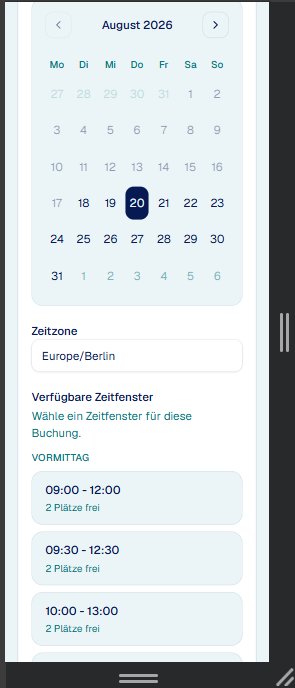
\includegraphics[width=0.25\textwidth]{Bilder/screenshot_reflow_320.png}
\caption{Terminauswahl bei einer Anzeigebreite von 320~px}
\label{fig:reflow_320}
\end{figure}

Kriterium~2.1.1 wurde mit \texttt{Tab}, \texttt{Umschalt+Tab},
\texttt{Enter}, \texttt{Leertaste} und \texttt{Esc} geprüft. Die
untersuchten Bereiche waren vollständig bedienbar. Beim Schließen des
Anmeldedialogs kehrt der Fokus jedoch nicht zur auslösenden
Schaltfläche zurück; dies betrifft Kriterium~2.4.3 und wurde nicht
bewertet.

Die Farbwerte des Designsystems sind paarweise definiert, sodass sich
jedes Verhältnis unmittelbar bestimmen lässt (vgl.
Abschnitt~\ref{subsec:designsystem}). Der Fließtext erreicht auf einer
Karte 16,5:1 und auf dem Seitenhintergrund 14,8:1, der gedämpfte Text
5,3:1 auf der Karte und 4,7:1 auf dem Seitenhintergrund. Sämtliche
Textpaarungen erfüllen damit Kriterium~1.4.3.

Beim Fokusring fallen Entwurf und Darstellung auseinander. Der
hinterlegte Wert ergäbe gegenüber einer Karte 3,6:1 und damit mehr als
die geforderten 3:1. Tatsächlich wird der Ring jedoch über eine
globale Regel mit halber Deckkraft gegen den Untergrund gemischt,
sodass nur 1,8:1 verbleiben. Er ist damit vorhanden und
sichtbar, aber nicht normkonform, und Kriterium~1.4.11 ist nicht
erfüllt. Diese Unterscheidung ist der eigentliche Ertrag der Messung:
Ob eine Anzeige wahrnehmbar ist, lässt sich betrachten; ob sie einen
Schwellenwert erreicht, nicht, und ein Blick auf die Farbwerte allein
genügt dafür ebenfalls nicht.

\section{Grenzen des Verfahrens}
\label{sec:grenzen_verfahren}

Die Evaluation wurde von einem einzelnen Evaluator durchgeführt und
stellt daher keine vollständige Erhebung dar
\cite{nielsen_molich_heuristic}. Da Evaluator und Entwickler dieselbe
Person sind, besteht zudem ein Risiko für eine unbewusste Orientierung
am vorgesehenen Nutzungspfad. Die heuristische Evaluation ersetzt
keinen Nutzertest. Außerdem wurden nur vier Erfolgskriterien der
Stufe~AA geprüft, weshalb keine vollständige WCAG-Konformität
abgeleitet werden kann.

\section{Bewertung der Ergebnisse}
\label{sec:bewertung}

Die Ergebnisse werden den nicht-funktionalen Anforderungen aus
Tabelle~\ref{tab:nichtfunktionale-anforderungen} gegenübergestellt.

Responsivität und Barrierefreiheit wurden anhand der relevanten
\acs{WCAG}-Kriterien geprüft. Die Kriterien~1.4.10 (Responsivität),
2.1.1 (Tastaturbedienung) und 1.4.3 (Textkontrast) sind erfüllt.
Nicht erfüllt ist Kriterium~1.4.11, da eine globale Regel den
Fokusring mit halber Deckkraft darstellt und er dadurch den
geforderten Wert unterschreitet. Die Korrektur betrifft lediglich
eine globale Regel.

Für die Performance ist der Programmcode auf 102 Dateien aufgeteilt,
von denen beim ersten Aufruf nur ein Teil übertragen wird. Die größte
Datei umfasst 230~kB und bleibt damit unter der vom Build-Werkzeug
genannten Schwelle von 500~kB.
Die Antwortzeiten wurden am gebauten Stand gemessen, jeweils vom Klick
bis zum nächsten Bildaufbau. Die Formularvalidierung, die ohne Anfrage
an das Backend auskommt, lag über vier Durchläufe zwischen 14 und
33~Millisekunden und damit unterhalb der geforderten 0,1~Sekunden. Der
Wechsel von der Produktliste auf eine Produktseite einschließlich des
Nachladens des zugehörigen Codestücks lag bei 10~Millisekunden und
damit unterhalb der geforderten Sekunde. Vorgänge mit Anfrage an das
Backend reagierten innerhalb von 17 bis 19~Millisekunden mit einem
Ladezustand; ihre Gesamtdauer hängt von der Antwortzeit der
Schnittstelle ab und ist nach Abschnitt~\ref{sec:abgrenzung} nicht
Gegenstand dieser Arbeit.

Die Sicherheit wurde nicht eigenständig geprüft. Die heuristische
Evaluation zeigte jedoch einen Befund (B1) beim rollenbasierten
Seitenschutz. Da die eigentliche Zugriffskontrolle serverseitig
erfolgt, dient der Frontend-Schutz hauptsächlich der Benutzerführung.

Die Wartbarkeit wurde anhand der Projektstruktur bewertet. Die
16 Funktionsbereiche unter \texttt{features/} folgen demselben Schema
aus Datenzugriff, Komponenten, Hooks, Seiten, Schemata und Typen,
jeweils beschränkt auf die benötigten Bestandteile (vgl.
Abschnitt~\ref{subsec:komponentenarchitektur}). Damit wurde die
geplante Architektur im gesamten Quellstand umgesetzt. Aussagen über
den zukünftigen Änderungsaufwand sind daraus jedoch nicht ableitbar.
    \chapter{Fazit und Ausblick}
\label{chap:fazit}

\section{Zusammenfassung der Ergebnisse}
\label{sec:zusammenfassung}

Diese Bachelorarbeit beschäftigt sich mit dem Entwurf und der
prototypischen Entwicklung des Frontends der Webanwendung
\textit{Bazario}. Ziel war eine rollenbasierte Single-Page
Application, über die sich Produkte kaufen und Dienstleistungen buchen
lassen, ohne dass der Nutzer zwischen zwei Anwendungen wechseln muss.

Am Anfang wurden die Motivation und die Anforderungen an das Frontend
behandelt und der Technologiestack darauf aufbauend begründet. Danach
folgten das Konzept mit Komponentenarchitektur, rollenbasiertem
Seitenschutz und \acs{UI}-Gestaltung sowie die Umsetzung ausgewählter
Funktionsbereiche mit React und TypeScript. Die entwickelte Oberfläche
deckt die Funktionsbereiche der drei im Frontend abgebildeten Rollen
ab, vom Katalog über den gemeinsamen Warenkorb für Produkte und
Buchungen bis zum Kontobereich, zum Nachrichtenbereich und zur
Verwaltung von Werbung; sie liegt in Deutsch, Englisch und Arabisch
vor.

Die Bewertung in Kapitel~\ref{chap:testen} erfolgte auf drei Wegen.
Die automatisierten Tests umfassen 36 Testdateien mit 134 Testfällen
sowie vier End-to-End-Tests und laufen fehlerfrei durch. Die
heuristische Evaluation ergab vierzehn Befunde, die sämtlich behoben
wurden. Von den vier geprüften Erfolgskriterien der
\acs{WCAG}~2.1 sind drei erfüllt; nicht erfüllt ist allein der
Kontrast des Fokusrings.

\section{Mögliche Erweiterungen und Ausblick}
\label{sec:ausblick}

Für die Weiterentwicklung des Frontends bieten sich mehrere
Erweiterungen an:

\begin{itemize}
  \item Eine eigene Administrationsoberfläche für Rollenwechselanträge,
  Freigaben, Gebühren und Auszahlungen.
  \item Erweiterte Suchfilter nach Preis, Ort und Verfügbarkeit.
  \item Die Korrektur des Fokusrings sowie eine automatisierte Prüfung
    der Kontrastwerte im Build-Vorgang.
  \item Die Anzeige des Lagerbestands mit einer Warnung im Warenkorb,
  wenn die gewählte Menge den Bestand übersteigt.
  \item Die Ergänzung von Lieferanschrift, Versandkosten und
  Sendungsstatus im Bestellprozess.
  \item Der Ausbau zur progressiven Web-App mit Benachrichtigungen zu
  Bestellungen, Buchungen und Nachrichten.
\end{itemize}
Rein im Frontend umsetzbar sind die Korrektur des Fokusrings sowie die
Administrationsoberfläche, da deren Funktionen bereits über die
Demonstrationsoberfläche bedient werden. Die übrigen Erweiterungen
setzen zusätzliche Schnittstellen im Backend voraus
\cite{alaatki_backend}.

Zusammenfassend stellt das entwickelte Frontend eine tragfähige und
erweiterbare Oberfläche für eine Plattform dar, die den Kauf von
Produkten und die Buchung von Dienstleistungen in einem gemeinsamen
Vorgang zusammenführt.
    % = = = = = = = = = = = = = = = = = = = = = = = =
    \bibliographystyle{dinat}
    \bibliography{literatur}
    % = = = = = = = = = = = = = = = = = = = = = = = =
\end{document}